% Options for packages loaded elsewhere
\PassOptionsToPackage{unicode}{hyperref}
\PassOptionsToPackage{hyphens}{url}
\PassOptionsToPackage{dvipsnames,svgnames,x11names}{xcolor}
%
\documentclass[
  letterpaper,
  DIV=11,
  numbers=noendperiod]{scrartcl}

\usepackage{amsmath,amssymb}
\usepackage{iftex}
\ifPDFTeX
  \usepackage[T1]{fontenc}
  \usepackage[utf8]{inputenc}
  \usepackage{textcomp} % provide euro and other symbols
\else % if luatex or xetex
  \usepackage{unicode-math}
  \defaultfontfeatures{Scale=MatchLowercase}
  \defaultfontfeatures[\rmfamily]{Ligatures=TeX,Scale=1}
\fi
\usepackage{lmodern}
\ifPDFTeX\else  
    % xetex/luatex font selection
\fi
% Use upquote if available, for straight quotes in verbatim environments
\IfFileExists{upquote.sty}{\usepackage{upquote}}{}
\IfFileExists{microtype.sty}{% use microtype if available
  \usepackage[]{microtype}
  \UseMicrotypeSet[protrusion]{basicmath} % disable protrusion for tt fonts
}{}
\makeatletter
\@ifundefined{KOMAClassName}{% if non-KOMA class
  \IfFileExists{parskip.sty}{%
    \usepackage{parskip}
  }{% else
    \setlength{\parindent}{0pt}
    \setlength{\parskip}{6pt plus 2pt minus 1pt}}
}{% if KOMA class
  \KOMAoptions{parskip=half}}
\makeatother
\usepackage{xcolor}
\setlength{\emergencystretch}{3em} % prevent overfull lines
\setcounter{secnumdepth}{-\maxdimen} % remove section numbering
% Make \paragraph and \subparagraph free-standing
\ifx\paragraph\undefined\else
  \let\oldparagraph\paragraph
  \renewcommand{\paragraph}[1]{\oldparagraph{#1}\mbox{}}
\fi
\ifx\subparagraph\undefined\else
  \let\oldsubparagraph\subparagraph
  \renewcommand{\subparagraph}[1]{\oldsubparagraph{#1}\mbox{}}
\fi

\usepackage{color}
\usepackage{fancyvrb}
\newcommand{\VerbBar}{|}
\newcommand{\VERB}{\Verb[commandchars=\\\{\}]}
\DefineVerbatimEnvironment{Highlighting}{Verbatim}{commandchars=\\\{\}}
% Add ',fontsize=\small' for more characters per line
\usepackage{framed}
\definecolor{shadecolor}{RGB}{241,243,245}
\newenvironment{Shaded}{\begin{snugshade}}{\end{snugshade}}
\newcommand{\AlertTok}[1]{\textcolor[rgb]{0.68,0.00,0.00}{#1}}
\newcommand{\AnnotationTok}[1]{\textcolor[rgb]{0.37,0.37,0.37}{#1}}
\newcommand{\AttributeTok}[1]{\textcolor[rgb]{0.40,0.45,0.13}{#1}}
\newcommand{\BaseNTok}[1]{\textcolor[rgb]{0.68,0.00,0.00}{#1}}
\newcommand{\BuiltInTok}[1]{\textcolor[rgb]{0.00,0.23,0.31}{#1}}
\newcommand{\CharTok}[1]{\textcolor[rgb]{0.13,0.47,0.30}{#1}}
\newcommand{\CommentTok}[1]{\textcolor[rgb]{0.37,0.37,0.37}{#1}}
\newcommand{\CommentVarTok}[1]{\textcolor[rgb]{0.37,0.37,0.37}{\textit{#1}}}
\newcommand{\ConstantTok}[1]{\textcolor[rgb]{0.56,0.35,0.01}{#1}}
\newcommand{\ControlFlowTok}[1]{\textcolor[rgb]{0.00,0.23,0.31}{#1}}
\newcommand{\DataTypeTok}[1]{\textcolor[rgb]{0.68,0.00,0.00}{#1}}
\newcommand{\DecValTok}[1]{\textcolor[rgb]{0.68,0.00,0.00}{#1}}
\newcommand{\DocumentationTok}[1]{\textcolor[rgb]{0.37,0.37,0.37}{\textit{#1}}}
\newcommand{\ErrorTok}[1]{\textcolor[rgb]{0.68,0.00,0.00}{#1}}
\newcommand{\ExtensionTok}[1]{\textcolor[rgb]{0.00,0.23,0.31}{#1}}
\newcommand{\FloatTok}[1]{\textcolor[rgb]{0.68,0.00,0.00}{#1}}
\newcommand{\FunctionTok}[1]{\textcolor[rgb]{0.28,0.35,0.67}{#1}}
\newcommand{\ImportTok}[1]{\textcolor[rgb]{0.00,0.46,0.62}{#1}}
\newcommand{\InformationTok}[1]{\textcolor[rgb]{0.37,0.37,0.37}{#1}}
\newcommand{\KeywordTok}[1]{\textcolor[rgb]{0.00,0.23,0.31}{#1}}
\newcommand{\NormalTok}[1]{\textcolor[rgb]{0.00,0.23,0.31}{#1}}
\newcommand{\OperatorTok}[1]{\textcolor[rgb]{0.37,0.37,0.37}{#1}}
\newcommand{\OtherTok}[1]{\textcolor[rgb]{0.00,0.23,0.31}{#1}}
\newcommand{\PreprocessorTok}[1]{\textcolor[rgb]{0.68,0.00,0.00}{#1}}
\newcommand{\RegionMarkerTok}[1]{\textcolor[rgb]{0.00,0.23,0.31}{#1}}
\newcommand{\SpecialCharTok}[1]{\textcolor[rgb]{0.37,0.37,0.37}{#1}}
\newcommand{\SpecialStringTok}[1]{\textcolor[rgb]{0.13,0.47,0.30}{#1}}
\newcommand{\StringTok}[1]{\textcolor[rgb]{0.13,0.47,0.30}{#1}}
\newcommand{\VariableTok}[1]{\textcolor[rgb]{0.07,0.07,0.07}{#1}}
\newcommand{\VerbatimStringTok}[1]{\textcolor[rgb]{0.13,0.47,0.30}{#1}}
\newcommand{\WarningTok}[1]{\textcolor[rgb]{0.37,0.37,0.37}{\textit{#1}}}

\providecommand{\tightlist}{%
  \setlength{\itemsep}{0pt}\setlength{\parskip}{0pt}}\usepackage{longtable,booktabs,array}
\usepackage{calc} % for calculating minipage widths
% Correct order of tables after \paragraph or \subparagraph
\usepackage{etoolbox}
\makeatletter
\patchcmd\longtable{\par}{\if@noskipsec\mbox{}\fi\par}{}{}
\makeatother
% Allow footnotes in longtable head/foot
\IfFileExists{footnotehyper.sty}{\usepackage{footnotehyper}}{\usepackage{footnote}}
\makesavenoteenv{longtable}
\usepackage{graphicx}
\makeatletter
\def\maxwidth{\ifdim\Gin@nat@width>\linewidth\linewidth\else\Gin@nat@width\fi}
\def\maxheight{\ifdim\Gin@nat@height>\textheight\textheight\else\Gin@nat@height\fi}
\makeatother
% Scale images if necessary, so that they will not overflow the page
% margins by default, and it is still possible to overwrite the defaults
% using explicit options in \includegraphics[width, height, ...]{}
\setkeys{Gin}{width=\maxwidth,height=\maxheight,keepaspectratio}
% Set default figure placement to htbp
\makeatletter
\def\fps@figure{htbp}
\makeatother

\KOMAoption{captions}{tableheading}
\makeatletter
\makeatother
\makeatletter
\makeatother
\makeatletter
\@ifpackageloaded{caption}{}{\usepackage{caption}}
\AtBeginDocument{%
\ifdefined\contentsname
  \renewcommand*\contentsname{Table of contents}
\else
  \newcommand\contentsname{Table of contents}
\fi
\ifdefined\listfigurename
  \renewcommand*\listfigurename{List of Figures}
\else
  \newcommand\listfigurename{List of Figures}
\fi
\ifdefined\listtablename
  \renewcommand*\listtablename{List of Tables}
\else
  \newcommand\listtablename{List of Tables}
\fi
\ifdefined\figurename
  \renewcommand*\figurename{Figure}
\else
  \newcommand\figurename{Figure}
\fi
\ifdefined\tablename
  \renewcommand*\tablename{Table}
\else
  \newcommand\tablename{Table}
\fi
}
\@ifpackageloaded{float}{}{\usepackage{float}}
\floatstyle{ruled}
\@ifundefined{c@chapter}{\newfloat{codelisting}{h}{lop}}{\newfloat{codelisting}{h}{lop}[chapter]}
\floatname{codelisting}{Listing}
\newcommand*\listoflistings{\listof{codelisting}{List of Listings}}
\makeatother
\makeatletter
\@ifpackageloaded{caption}{}{\usepackage{caption}}
\@ifpackageloaded{subcaption}{}{\usepackage{subcaption}}
\makeatother
\makeatletter
\@ifpackageloaded{tcolorbox}{}{\usepackage[skins,breakable]{tcolorbox}}
\makeatother
\makeatletter
\@ifundefined{shadecolor}{\definecolor{shadecolor}{rgb}{.97, .97, .97}}
\makeatother
\makeatletter
\makeatother
\makeatletter
\makeatother
\ifLuaTeX
  \usepackage{selnolig}  % disable illegal ligatures
\fi
\IfFileExists{bookmark.sty}{\usepackage{bookmark}}{\usepackage{hyperref}}
\IfFileExists{xurl.sty}{\usepackage{xurl}}{} % add URL line breaks if available
\urlstyle{same} % disable monospaced font for URLs
\hypersetup{
  colorlinks=true,
  linkcolor={blue},
  filecolor={Maroon},
  citecolor={Blue},
  urlcolor={Blue},
  pdfcreator={LaTeX via pandoc}}

\author{}
\date{}

\begin{document}
\ifdefined\Shaded\renewenvironment{Shaded}{\begin{tcolorbox}[interior hidden, sharp corners, borderline west={3pt}{0pt}{shadecolor}, boxrule=0pt, enhanced, frame hidden, breakable]}{\end{tcolorbox}}\fi

\hypertarget{sec-noncovalent-functionalisation}{%
\section{Non-Covalent Functionalisation of Carbon Nanotube \& Graphene
Films}\label{sec-noncovalent-functionalisation}}

\hypertarget{introduction}{%
\subsection{Introduction}\label{introduction}}

In \textbf{?@sec-fabrication}, methods of fabricating carbon nanotube
and graphene devices were discussed, and in
\textbf{?@sec-pristine-characteristics}, it was demonstrated that these
devices are highly sensitive to environmental changes in an aqueous
environment. However, for specific sensing, the devices require
biochemical functionalisation. The sensing signal is picked up by
attached receptors, while the transistors act as transducers for the
received signal. Receptors previously used with carbon nanotube and
graphene devices include aptamers {[}@Khan2021; @Nguyen2021;
@Shkodra2021; @Nekrasov2021; @Mishyn2022; @Cassie2023{]} and a range of
proteins {[}@Lerner2014; @Ahn2020; @Tong2020; @Wang2020{]}, including
animal odorant receptors {[}@Goldsmith2011; @Lee2018; @Murugathas2019a;
@Murugathas2020; @Moon2020; @Yoo2022{]}. A common approach to attaching
receptors to the transducer involves the use of a linker molecule to
tether the receptor to the transducer. Verifying that this linker
molecule is bridging between the transducer and the receptor element is
important for a complete understanding of the behaviour of these
sensors. This verification involves providing evidence for effective
attachment of linker molecule to the transducing device channel, then
showing successful tethering of odorant receptors and other biomolecules
to the attached linker molecule.

This chapter therefore takes some time exploring the following selection
of available linker molecules for specific biosensing: 1-Pyrenebutanoic
Acid N-hydroxysuccinimide Ester (PBASE), 1-Pyrenebutyric Acid (PBA),
Pyrene-PEG-NTA (PPN) and Pyrene-PEG-Biotin (PPB). The mechanisms
underlying functionalisation with each linker are described. A
literature review and analysis techniques including Raman spectroscopy,
fluorescence microscopy and electrical characterisation are used to
understand the impact of various experimental parameters on the
functionalisation process. Electrical characterisation of linker
attachment to the transducer was also performed to act as a comparison
tool when performing functionalisation with insect odorant receptors.
Numerous obstacles to successful functionalisation are identified and
discussed, including PBASE hydrolysis, linker coverage, non-specific
attachment, photoresist contamination, channel hydrophobicity and the
coffee-ring effect. Approaches to overcome these obstacles were
identified, tested and the results characterised. This process provided
assurance that successful attachment of linker molecule to the carbon
nanotube network or graphene region could be achieved.

\hypertarget{sec-PBASE}{%
\subsection{Attachment of 1-Pyrenebutanoic Acid N-Hydroxysuccinimide
Ester}\label{sec-PBASE}}

\hypertarget{sec-pi-stacking}{%
\subsubsection{Pi-stacking}\label{sec-pi-stacking}}

Pi-stacking or \(\pi-\pi\) interaction is a specific type of
non-covalent bonding which occurs due to dispersion forces between
unsaturated polycyclic molecules {[}@Perez2015{]}. It has been argued
that this label is unhelpfully specific and a misrepresentation of what
can be simply classed as a type of Van der Waals bonding
{[}@Martinez2012; @Perez2015{]}. However, as the use of the term is
widespread in the literature, it is also used here for the sake of
clarity. A wide range of linker molecules with aromatic moieties, such
as pyrene, have been used for modification of polycyclic carbon
nanotubes and graphene via pi-stacking {[}@Hermanson2013-16; @Perez2015;
@Zhou2019; @Mishyn2022{]}. Pyrene-based pi-stacking underlies all the
functionalisation processes used in this thesis.
Figure~\ref{fig-pi-interaction-cnt} demonstrates how a pyrene-based
linker molecule can be used to attach a receptor element to a thin-film
transducer. The linker element attaches to the biomolecule via covalent
bonding with a nucleophilic functional group; linker attachment can
occur via biomolecule aminos, carboxyls, hydroxyls, thiols/sulfhydryls,
phenols, imidazoles and so on {[}@Fruh2011; @Dung2018{]}.

\begin{figure}

{\centering 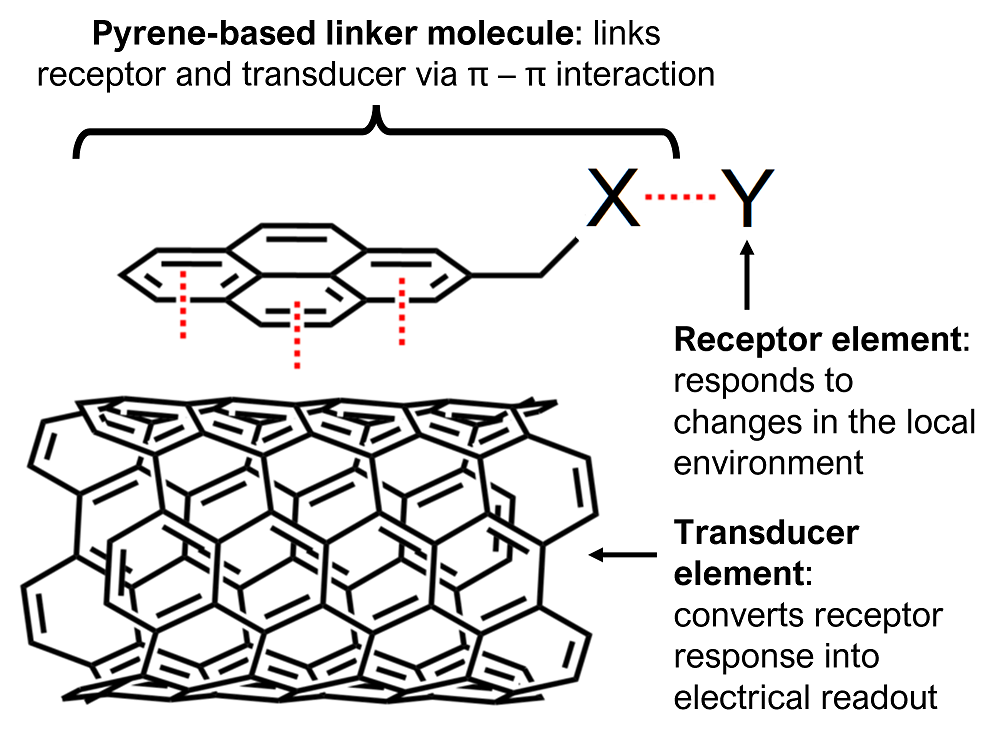
\includegraphics[width=0.6\textwidth,height=\textheight]{figures/ch6/pyrene-cnt.png}

}

\caption[Attachment of pyrene-based linker molecule pyrene-X and
receptor Y to a carbon nanotube, representing the transducer element of
a field-effect transistor.]{\label{fig-pi-interaction-cnt}Attachment of
pyrene-based linker molecule pyrene-X and receptor Y to a carbon
nanotube, representing the transducer element of a field-effect
transistor. Figure adapted from {[}@Carbonnanotube{]}, used under the CC
BY-SA 4.0 license.}

\end{figure}

\hypertarget{sec-PBASE-attachment}{%
\subsubsection{Comparing Attachment
Methods}\label{sec-PBASE-attachment}}

1-pyrenebutanoic acid N-hydroxysuccinimide ester (also known as
1-pyrenebutyric acid N-hydroxysuccinimide ester and 1-pyrenebutanoic
acid succinimidyl ester, and by the acronyms PBASE, PBSE, PyBASE, PASE,
PYSE, PSE, Pyr-NHS and PANHS) is a pyrene-based linker molecule commonly
used for tethering biomolecules to the carbon rings of graphene and
carbon nanotubes. A ball-and-stick model of the PBASE molecule is shown
in Figure~\ref{fig-pbase-structure}. The pyrene moiety, highlighted blue
in Figure~\ref{fig-pbase-structure}, non-covalently bonds to the carbon
rings of the transducer. Previous modelling has shown that when PBASE
attaches to graphene, it may take on one of two different locally stable
conformations (one straight, one bent) {[}@Oishi2022{]}. The
N-hydroxysuccinimide (NHS) ester group, found within the structure
highlighted red in Figure~\ref{fig-pbase-structure}, can undergo a
nucleophilic substitution reaction with primary amines attached to
biomolecules, tethering them with an amide or imide bond {[}@Chen2001;
@Hermanson2013-16; @Hermanson2013-3; @Shkodra2021; @Mishyn2022{]}.

\begin{figure}

{\centering 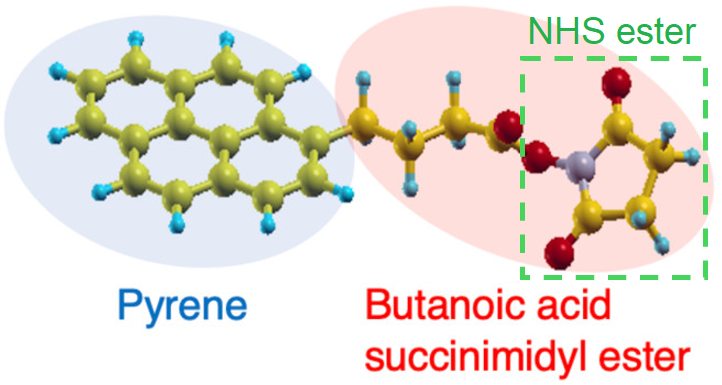
\includegraphics[width=0.9\textwidth,height=\textheight]{figures/ch6/PBASE_edit.png}

}

\caption[Structure of 1-pyrenebutanoic acid N-hydroxysuccinimide ester
(PBASE).]{\label{fig-pbase-structure}Structure of 1-pyrenebutanoic acid
N-hydroxysuccinimide ester (PBASE) visualised in XCrySDen software
{[}@Kokalj1999{]}. Blue corresponds to hydrogen, yellow to carbon, red
to oxygen and grey to nitrogen. The NHS ester is the ring structure on
the right hand side of the figure. Figure reproduced from
{[}@Oishi2022{]}, used under the CC BY-NC-ND 4.0 license.}

\end{figure}

The non-covalent functionalisation of proteins onto a single-walled
carbon nanotube using PBASE was first reported by Chen \emph{et al.} in
2001 {[}@Chen2001{]}. Two successful methods for protein
functionalisation and immobilisation were reported, with the only
differences being the solvent used to dissolve the PBASE powder
(dimethylformamide, methanol) and the final concentration of the
resulting solutions (6 mM, 1 mM respectively). PBASE powder appears to
dissolve poorly in methanol at higher concentrations, which might
explain the use of different concentrations of PBASE with each solvent.
An extensive comparison of methods used in the literature for PBASE
functionalisation of carbon nanotube and graphene devices with aptamers
and proteins is given in \textbf{?@tbl-pbase-functionalisation}. Several
listed works directly cite Chen \emph{et al.} when discussing
functionalisation with PBASE {[}@Cella2010; @Ohno2010; @Zheng2016{]}.
The other works listed do not explicitly reference Chen \emph{et al.} in
their methodology; however, the frequency of methods describing the use
of 6 mM PBASE in dimethylformamide (DMF) and 1 mM PBASE in methanol
indicate that other groups typically emulate the original process from
Chen \emph{et al.}

However, it is also apparent from \textbf{?@tbl-pbase-functionalisation}
that there is a large degree of variation in the methods used for PBASE
functionalisation. Various electrical characterisation, microscopy and
spectroscopy techniques have been used to demonstrate successful
functionalisation. Until recently, there has been little justification
provided for the selection of variables used in the functionalisation
procedure (\emph{e.g.} length of time submerged in solvent containing
PBASE), despite the widespread use of this process in the literature
{[}@Hinnemo2017; @Zhen2018; @Wang2020{]}. Furthermore, a detailed
investigation of PBASE functionalisation process variables has only been
undertaken for graphene-based devices {[}@Zhen2018; @Hao2020; @Wang2020;
@Mishyn2022{]}. This is surprising, given that multiple sources make an
explicit link between sensitivity of functionalised devices and the
density of surface functionalisation with PBASE {[}@White2008;
@Hermanson2013-3; @Chen2014{]}.

Zhen \emph{et al.} {[}@Zhen2018{]}, Wang \emph{et al.} {[}@Wang2020{]}
and Mishyn \emph{et al.} {[}@Mishyn2022{]} have all claimed that
carefully tuning the surface concentration of PBASE is required to avoid
multilayer coverage of the graphene surface, as this negatively impacts
sensing. Mishyn \emph{et al.} {[}@Mishyn2022{]} used cyclic voltammetry
to demonstrate that less receptor attachment to the graphene surface
occurs when multiple layers of PBASE are present. However, none of these
groups have presented analyte sensing results from their functionalised
graphene devices. In contrast, Hao \emph{et al.} {[}@Hao2020{]} found
that maximising the PBASE surface coverage of a channel resulted in more
sensitive aptameric sensing. The inconsistency in these recent findings
mean more work is needed to understand the PBASE functionalisation
process and achieve optimal biosensor sensitivity.

It may also be the case that a specific functionalisation process is
required for optimal sensitivity with the use of a specific type of
receptor.

Once fastened to a bioreceptor via an amide or imide bond, the
attachment to the linker molecule is not easily broken. However, prior
to use in functionalisation processes, the NHS ester may react with any
water present. This ester hydrolysis converts PBASE to its corresponding
carboxylic acid, 1-pyrenebutyric acid (PBA), leaving it unavailable to
react further with amine groups {[}@Hermanson2013-3; @Hermanson2013-5;
@Mishyn2022{]}. If the amine group functionalisation is performed at
close to neutral pH, within a \(\sim\) 1 hour period, and with a high
concentration of bioreceptor present, competing hydrolysis should not
have a significantly adverse impact on the functionalisation process
{[}@Hermanson2013-3{]}. If PBASE is exposed to water during storage,
1-ethyl-3-(3-dimethylaminopropyl)carbodiimide (EDC) can be used to
restore the NHS ester and enable the substitution reaction to take place
(see Section~\ref{sec-PBA}).

\hypertarget{sec-PBASE-purity}{%
\subsubsection{Examining 1-Pyrenebutanoic Acid N-Hydroxysuccinimide
Ester Purity}\label{sec-PBASE-purity}}

I purchased PBASE from two suppliers, Sigma-Aldrich and Setareh Biotech.
Sigma-Aldrich listed DMF and methanol as suitable solvents for
dissolving PBASE, alongside chloroform and dimethyl sulfoxide (DMSO).
Setareh Biotech indicated methanol can be used for dissolving PBASE. The
two suppliers had conflicting information for suitable storage of PBASE,
where Sigma recommended room temperature storage, while Setareh Biotech
recommended storage of \(-5\) to \(-30\) °C alongside protection from
light and moisture. Nuclear magnetic resonance (NMR) spectroscopy was
used to verify the purity of PBASE from various suppliers. As water can
react with PBASE to form unwanted byproducts, it appears that protection
from moisture is particularly important. A particular emphasis was
placed on detecting water presence in the received samples, considering
the long travel time of the PBASE with uncertain storage conditions.

Figure~\ref{fig-pbase-nmr} compares the shapes of hydrogen NMR spectra
of PBASE from each supplier when dissolved in deuterated DMSO, alongside
a blank deuterated DMSO spectrum. Both PBASE samples possessed
characteristic chemical shift features between \(2.1-2.2\) ppm,
\(2.8-2.9\) ppm, and \(3.4-3.5\) ppm. These chemical shifts roughly
correspond to those seen in previous NMR spectra for PBASE {[}@NMR2{]}.
The feature at 2.5 ppm represents the deuterated DMSO solvent, while the
single peak between \(3.3-3.4\) ppm represents the water present in the
sample. By comparing the area of these peaks, a rough estimate of the
amount of water originally present in the PBASE sample can be obtained.

\begin{figure}

\begin{minipage}[t]{0.03\linewidth}

{\centering 

\raisebox{-\height}{


\includegraphics{figures/(a).png}

}

}

\end{minipage}%
%
\begin{minipage}[t]{0.01\linewidth}

{\centering 

~

}

\end{minipage}%
%
\begin{minipage}[t]{0.92\linewidth}

{\centering 

\raisebox{-\height}{

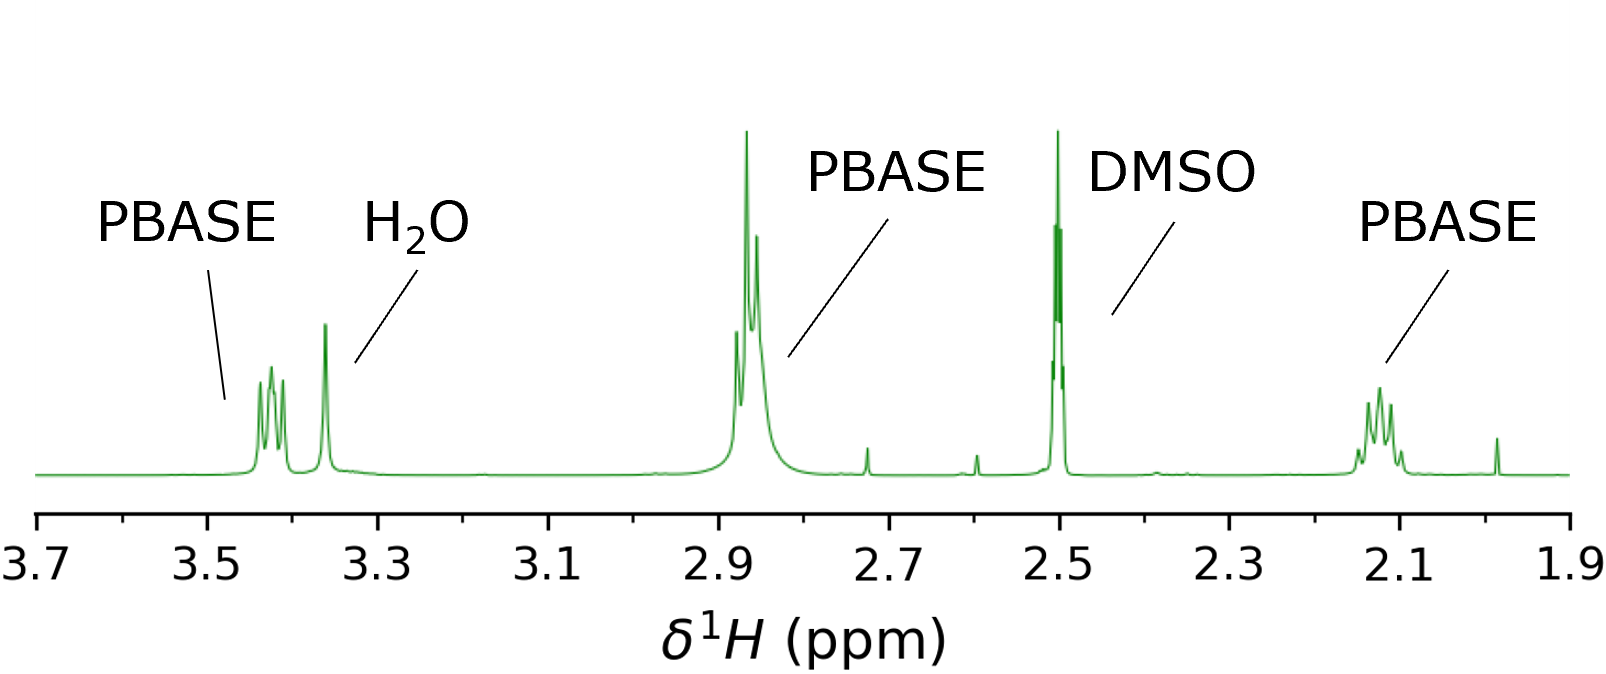
\includegraphics{figures/ch6/labelled_modified_sigma_pbase_nmr.png}

}

}

\end{minipage}%
%
\begin{minipage}[t]{0.04\linewidth}

{\centering 

~

}

\end{minipage}%
\newline
\begin{minipage}[t]{0.03\linewidth}

{\centering 

\raisebox{-\height}{


\includegraphics{figures/(b).png}

}

}

\end{minipage}%
%
\begin{minipage}[t]{0.01\linewidth}

{\centering 

~

}

\end{minipage}%
%
\begin{minipage}[t]{0.92\linewidth}

{\centering 

\raisebox{-\height}{

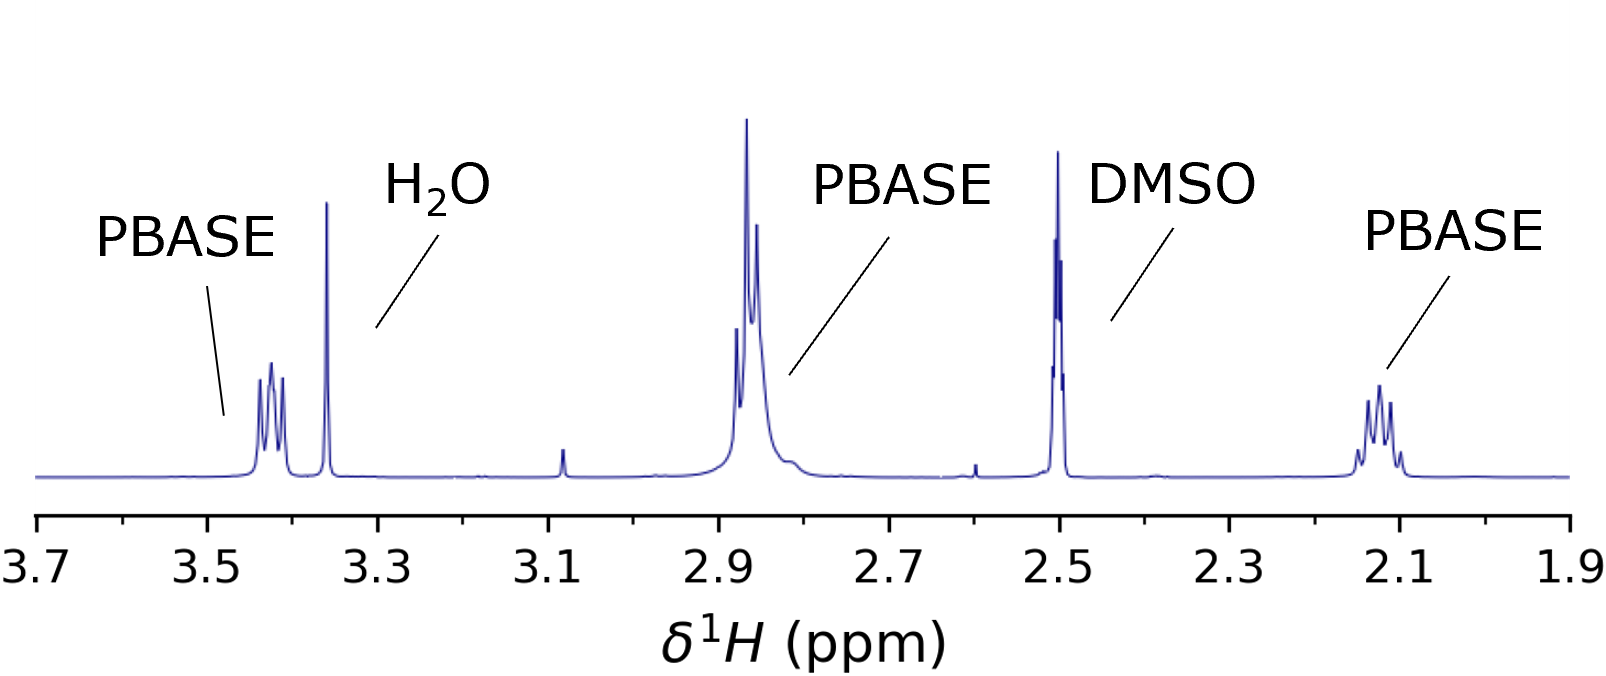
\includegraphics{figures/ch6/labelled_modified_setareh_pbase_nmr.png}

}

}

\end{minipage}%
%
\begin{minipage}[t]{0.04\linewidth}

{\centering 

~

}

\end{minipage}%
\newline
\begin{minipage}[t]{0.03\linewidth}

{\centering 

\raisebox{-\height}{


\includegraphics{figures/(c).png}

}

}

\end{minipage}%
%
\begin{minipage}[t]{0.01\linewidth}

{\centering 

~

}

\end{minipage}%
%
\begin{minipage}[t]{0.92\linewidth}

{\centering 

\raisebox{-\height}{

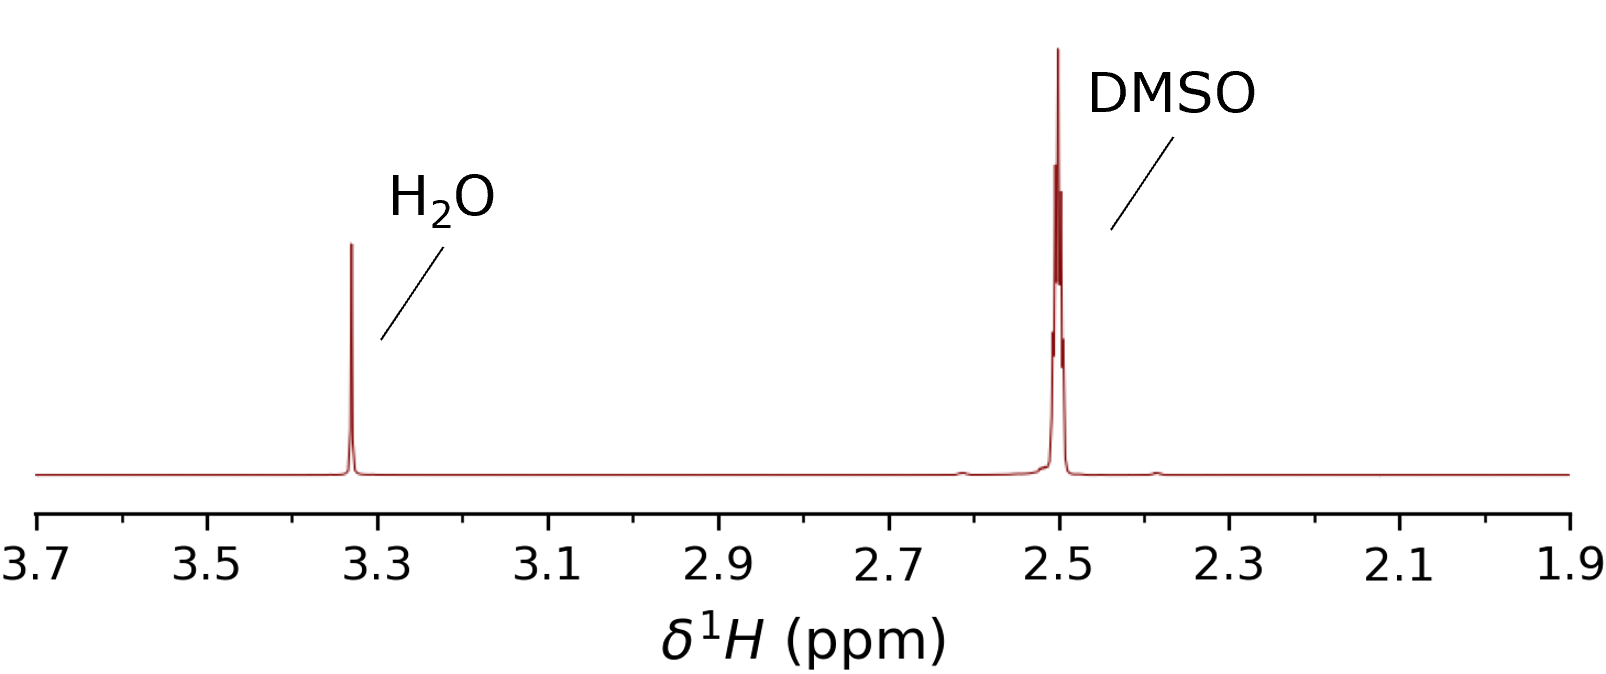
\includegraphics{figures/ch6/labelled_modified_dmso_nmr.png}

}

}

\end{minipage}%
%
\begin{minipage}[t]{0.04\linewidth}

{\centering 

~

}

\end{minipage}%

\caption[\(^{1}\)H Nuclear Magnetic Resonance (NMR) spectra of
commercially purchased PBASE in the alkyl region, using DMSO-d\(_6\) as
the NMR solvent.]{\label{fig-pbase-nmr}\(^{1}\)H Nuclear Magnetic
Resonance (NMR) spectra in the alkyl region. Spectra were taken using
DMSO-d\(_6\) as the NMR solvent. (a) and (b) show NMR spectrum for
commercially purchased PBASE, from Sigma-Aldrich and Setareh Biotech
respectively, while (c) shows the blank spectrum taken with only
DMSO-d\(_6\) present. Spectra were taken by Jennie Ramirez-Garcia,
School of Chemical and Physical Sciences, Te Herenga Waka \(-\) Victoria
University of Wellington. Unlabelled peaks correspond to sample
impurities.}

\end{figure}

The H\(_{2}\)O:DMSO ratio is 1:7 in the blank spectrum, but \(\sim\) 1:3
in the provided samples, possibly indicating the introduction of water
to the PBASE during production or storage. However, DMSO is strongly
hygroscopic and slight differences in DMSO storage time, as well as
differences in humidity during sample preparation, may have had a
significant impact on this result {[}@Lebel1962{]}. Other impurities are
also seen on both PBASE spectra, though their small size indicates they
make up only a small percentage of each sample. Strack \emph{et al.}
{[}@Strack2013{]} recommend leaving frozen PBASE at room temperature for
15 minutes before exposing it to air to prevent condensation near the
PBASE, as this can cause unnecessary H\(_2\)O contamination.

\hypertarget{sec-PBASE-electrical-characterisation}{%
\subsubsection{Electrical
Characterisation}\label{sec-PBASE-electrical-characterisation}}

The transfer characteristics of the carbon nanotube or graphene
transistor are often used to verify successful functionalisation and
make a statement about the effects of chemical modification. However,
this verification usually does not account for the effects of exposing
the transistor channel to solvent.
Figure~\ref{fig-PBASE-vs-solvent-only} (a) and
Figure~\ref{fig-PBASE-vs-solvent-only} (b) show that by exposing a
steam-deposited carbon nanotube network channel to solvents commonly
used in PBASE functionalisation processes
(\textbf{?@tbl-pbase-functionalisation}), such as methanol (MeOH) or
dimethyl sulfoxide (DMSO), a significant negative shift in channel
threshold voltage occurs even after thorough rinsing with deionised
water. It appears that the carbon nanotubes have adsorped solvent which
persists even after thoroughly rinsing the device. From the shape of the
change in the transfer curve, it seems the residual polar solvent
molecules capacitively gate the channel {[}@Artyukhin2006;
@Heller2008{]}. Besteman \emph{et al.} reported observing a similar
effect from prolonged exposure of a single carbon nanotube to
dimethylformamide (DMF) {[}@Besteman2003{]}.

\begin{figure}

\begin{minipage}[t]{0.03\linewidth}

{\centering 

\raisebox{-\height}{


\includegraphics{figures/(a).png}

}

}

\end{minipage}%
%
\begin{minipage}[t]{0.01\linewidth}

{\centering 

~

}

\end{minipage}%
%
\begin{minipage}[t]{0.45\linewidth}

{\centering 

\raisebox{-\height}{

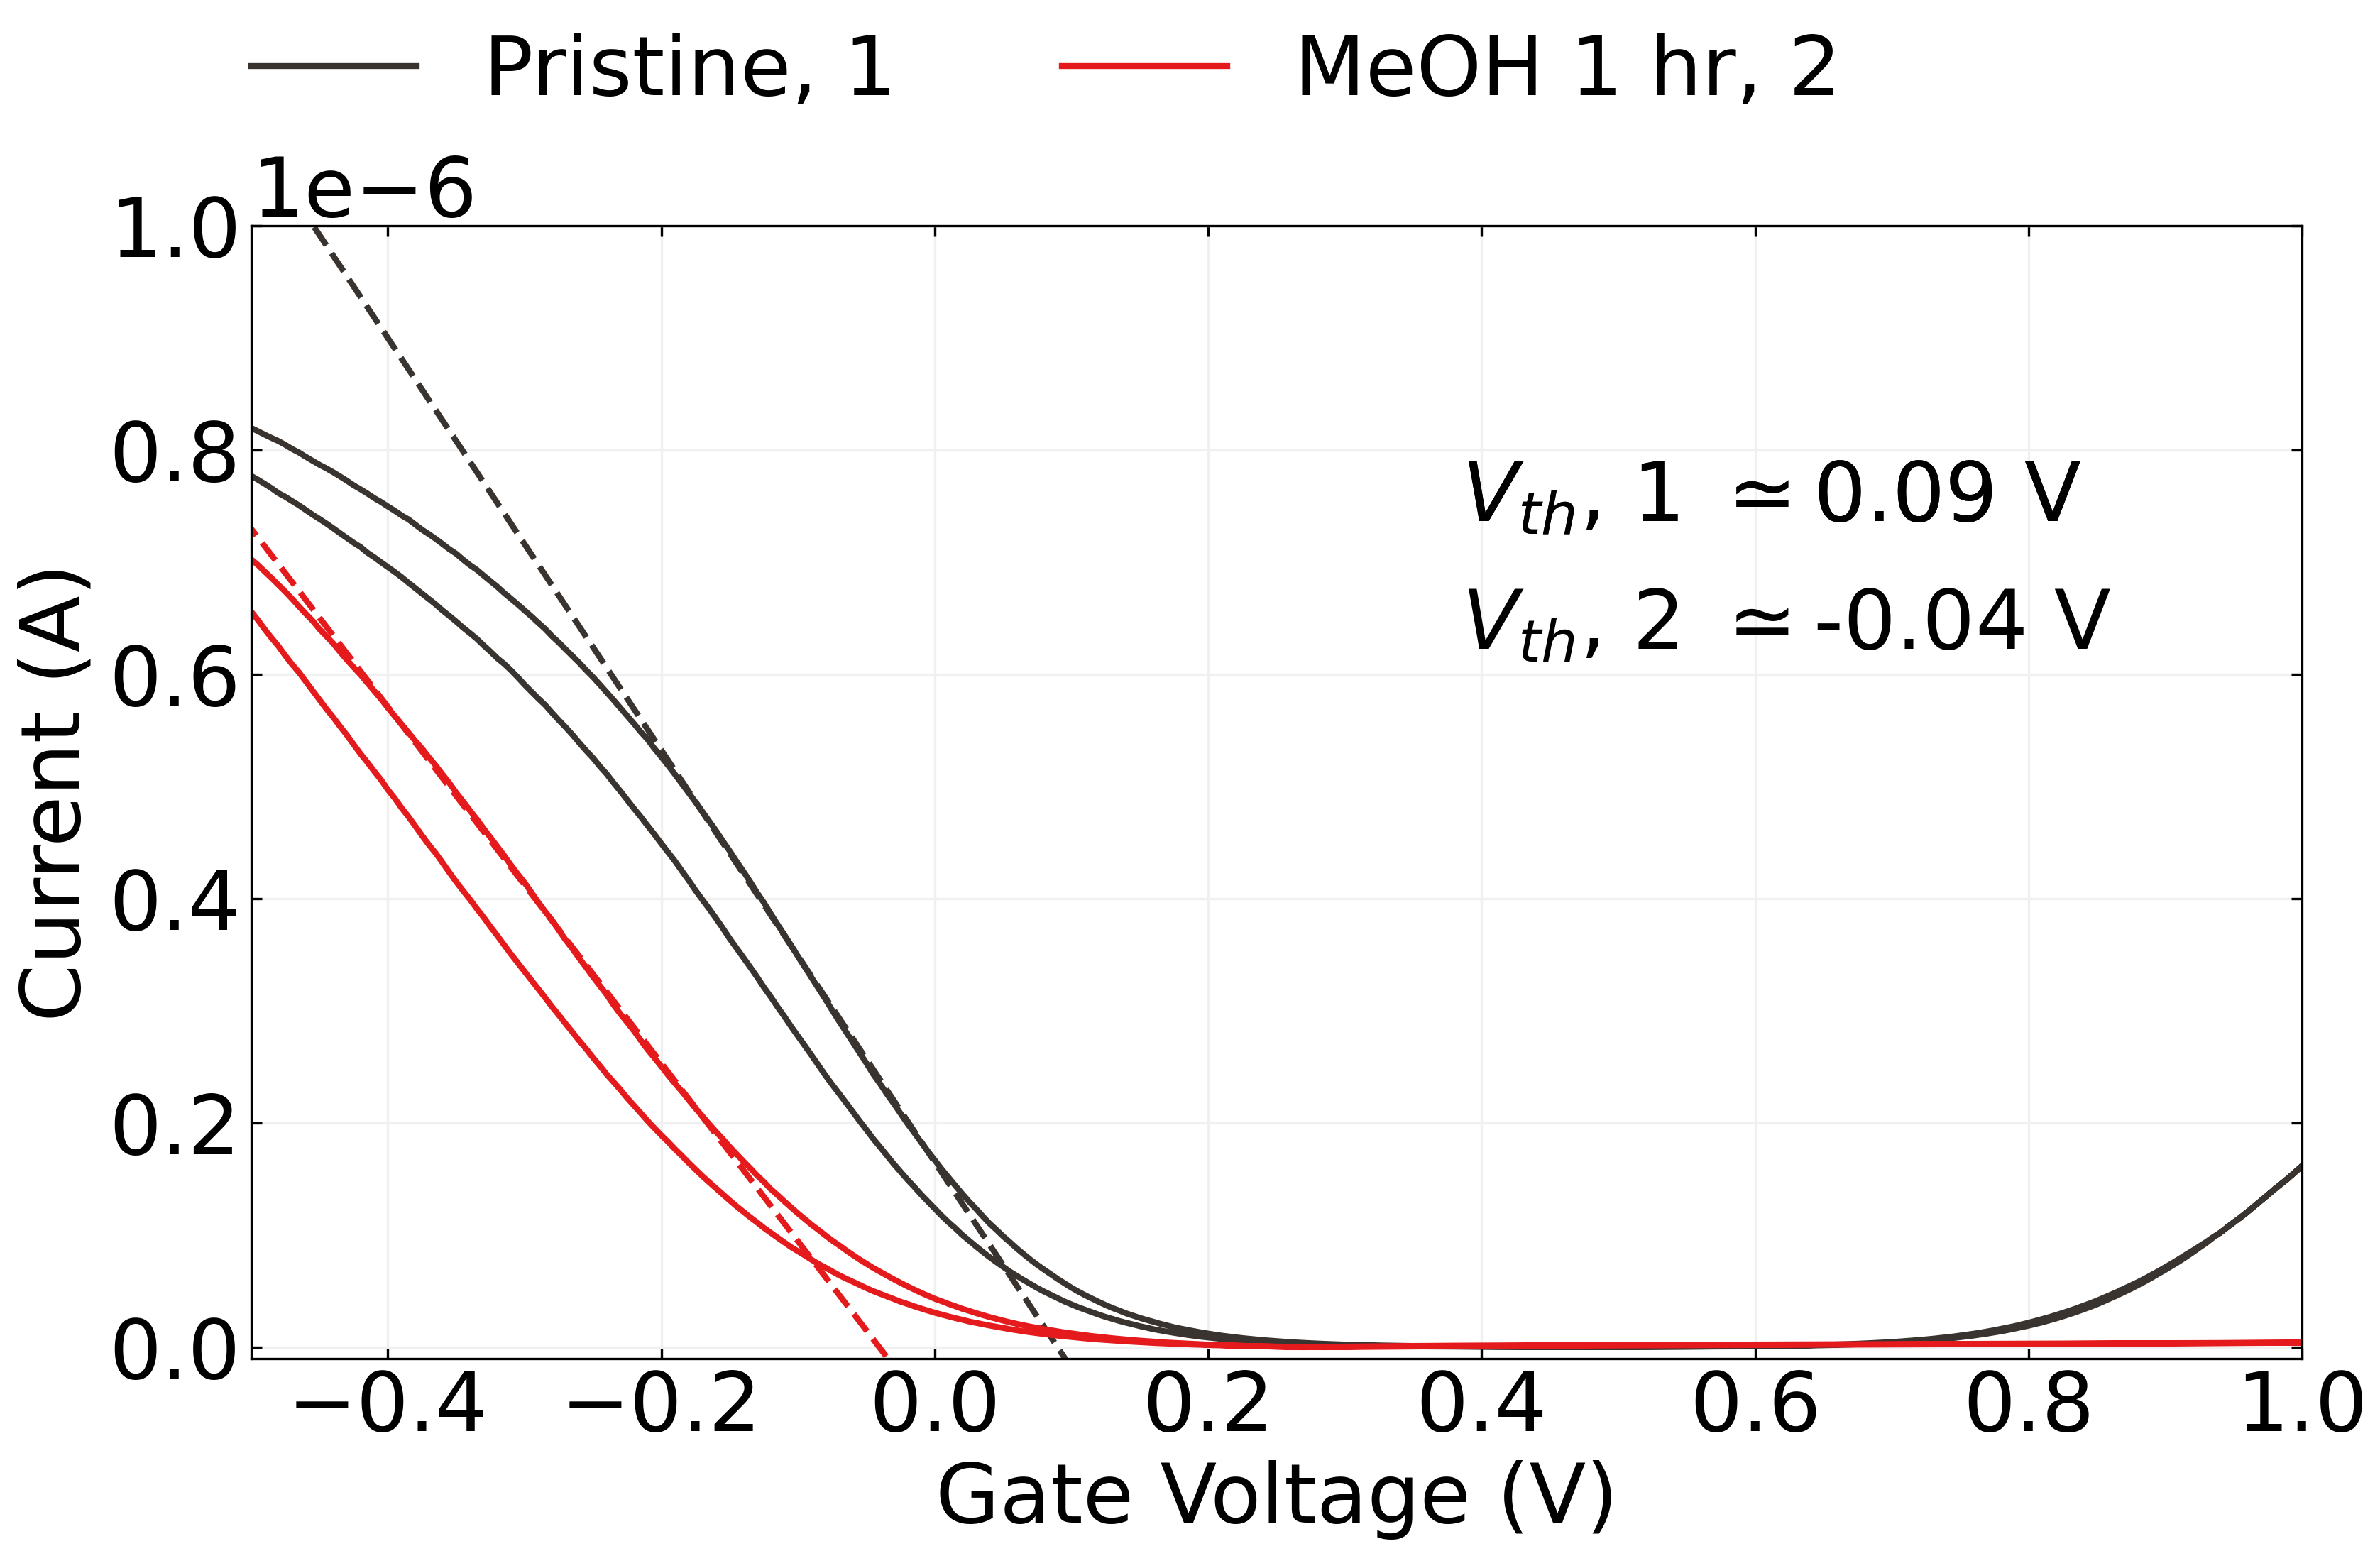
\includegraphics{figures/ch6/Q23D5_ch1_MeOHonly.png}

}

}

\end{minipage}%
%
\begin{minipage}[t]{0.01\linewidth}

{\centering 

~

}

\end{minipage}%
%
\begin{minipage}[t]{0.03\linewidth}

{\centering 

\raisebox{-\height}{


\includegraphics{figures/(b).png}

}

}

\end{minipage}%
%
\begin{minipage}[t]{0.01\linewidth}

{\centering 

~

}

\end{minipage}%
%
\begin{minipage}[t]{0.45\linewidth}

{\centering 

\raisebox{-\height}{

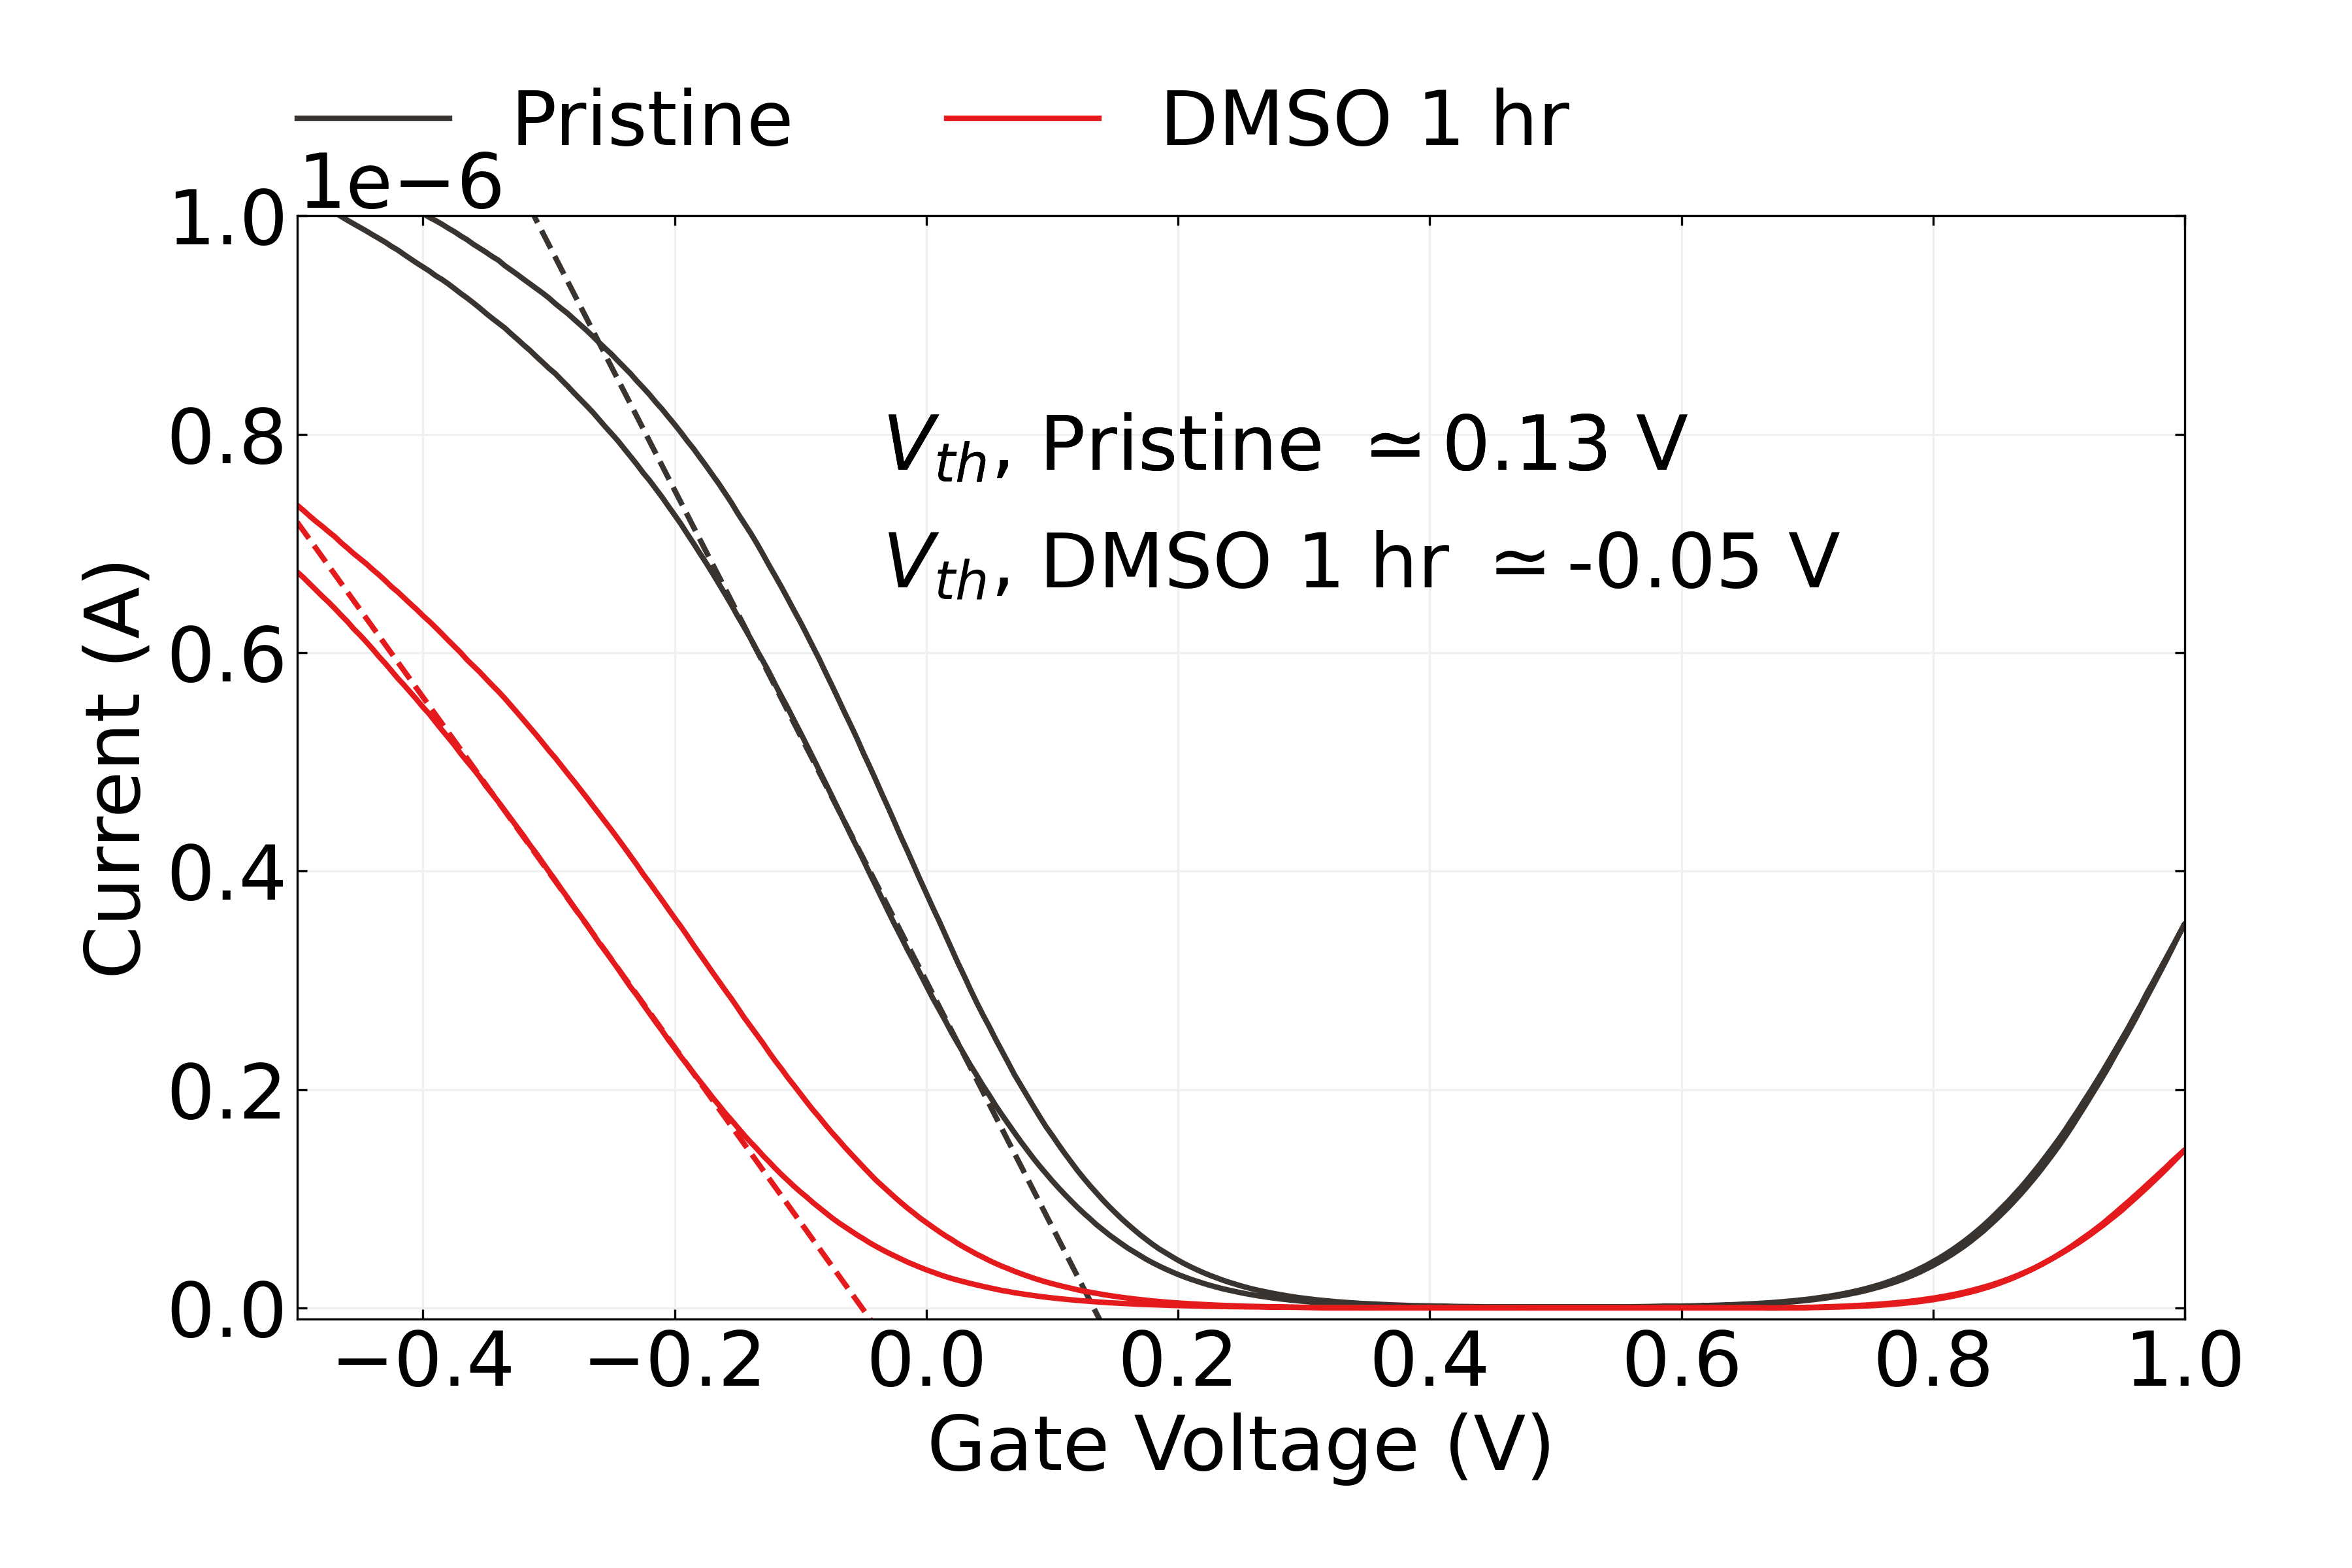
\includegraphics{figures/ch6/Q23D12_ch1_DMSOonly.png}

}

}

\end{minipage}%
%
\begin{minipage}[t]{0.01\linewidth}

{\centering 

~

}

\end{minipage}%
\newline
\begin{minipage}[t]{0.03\linewidth}

{\centering 

\raisebox{-\height}{


\includegraphics{figures/(c).png}

}

}

\end{minipage}%
%
\begin{minipage}[t]{0.01\linewidth}

{\centering 

~

}

\end{minipage}%
%
\begin{minipage}[t]{0.45\linewidth}

{\centering 

\raisebox{-\height}{

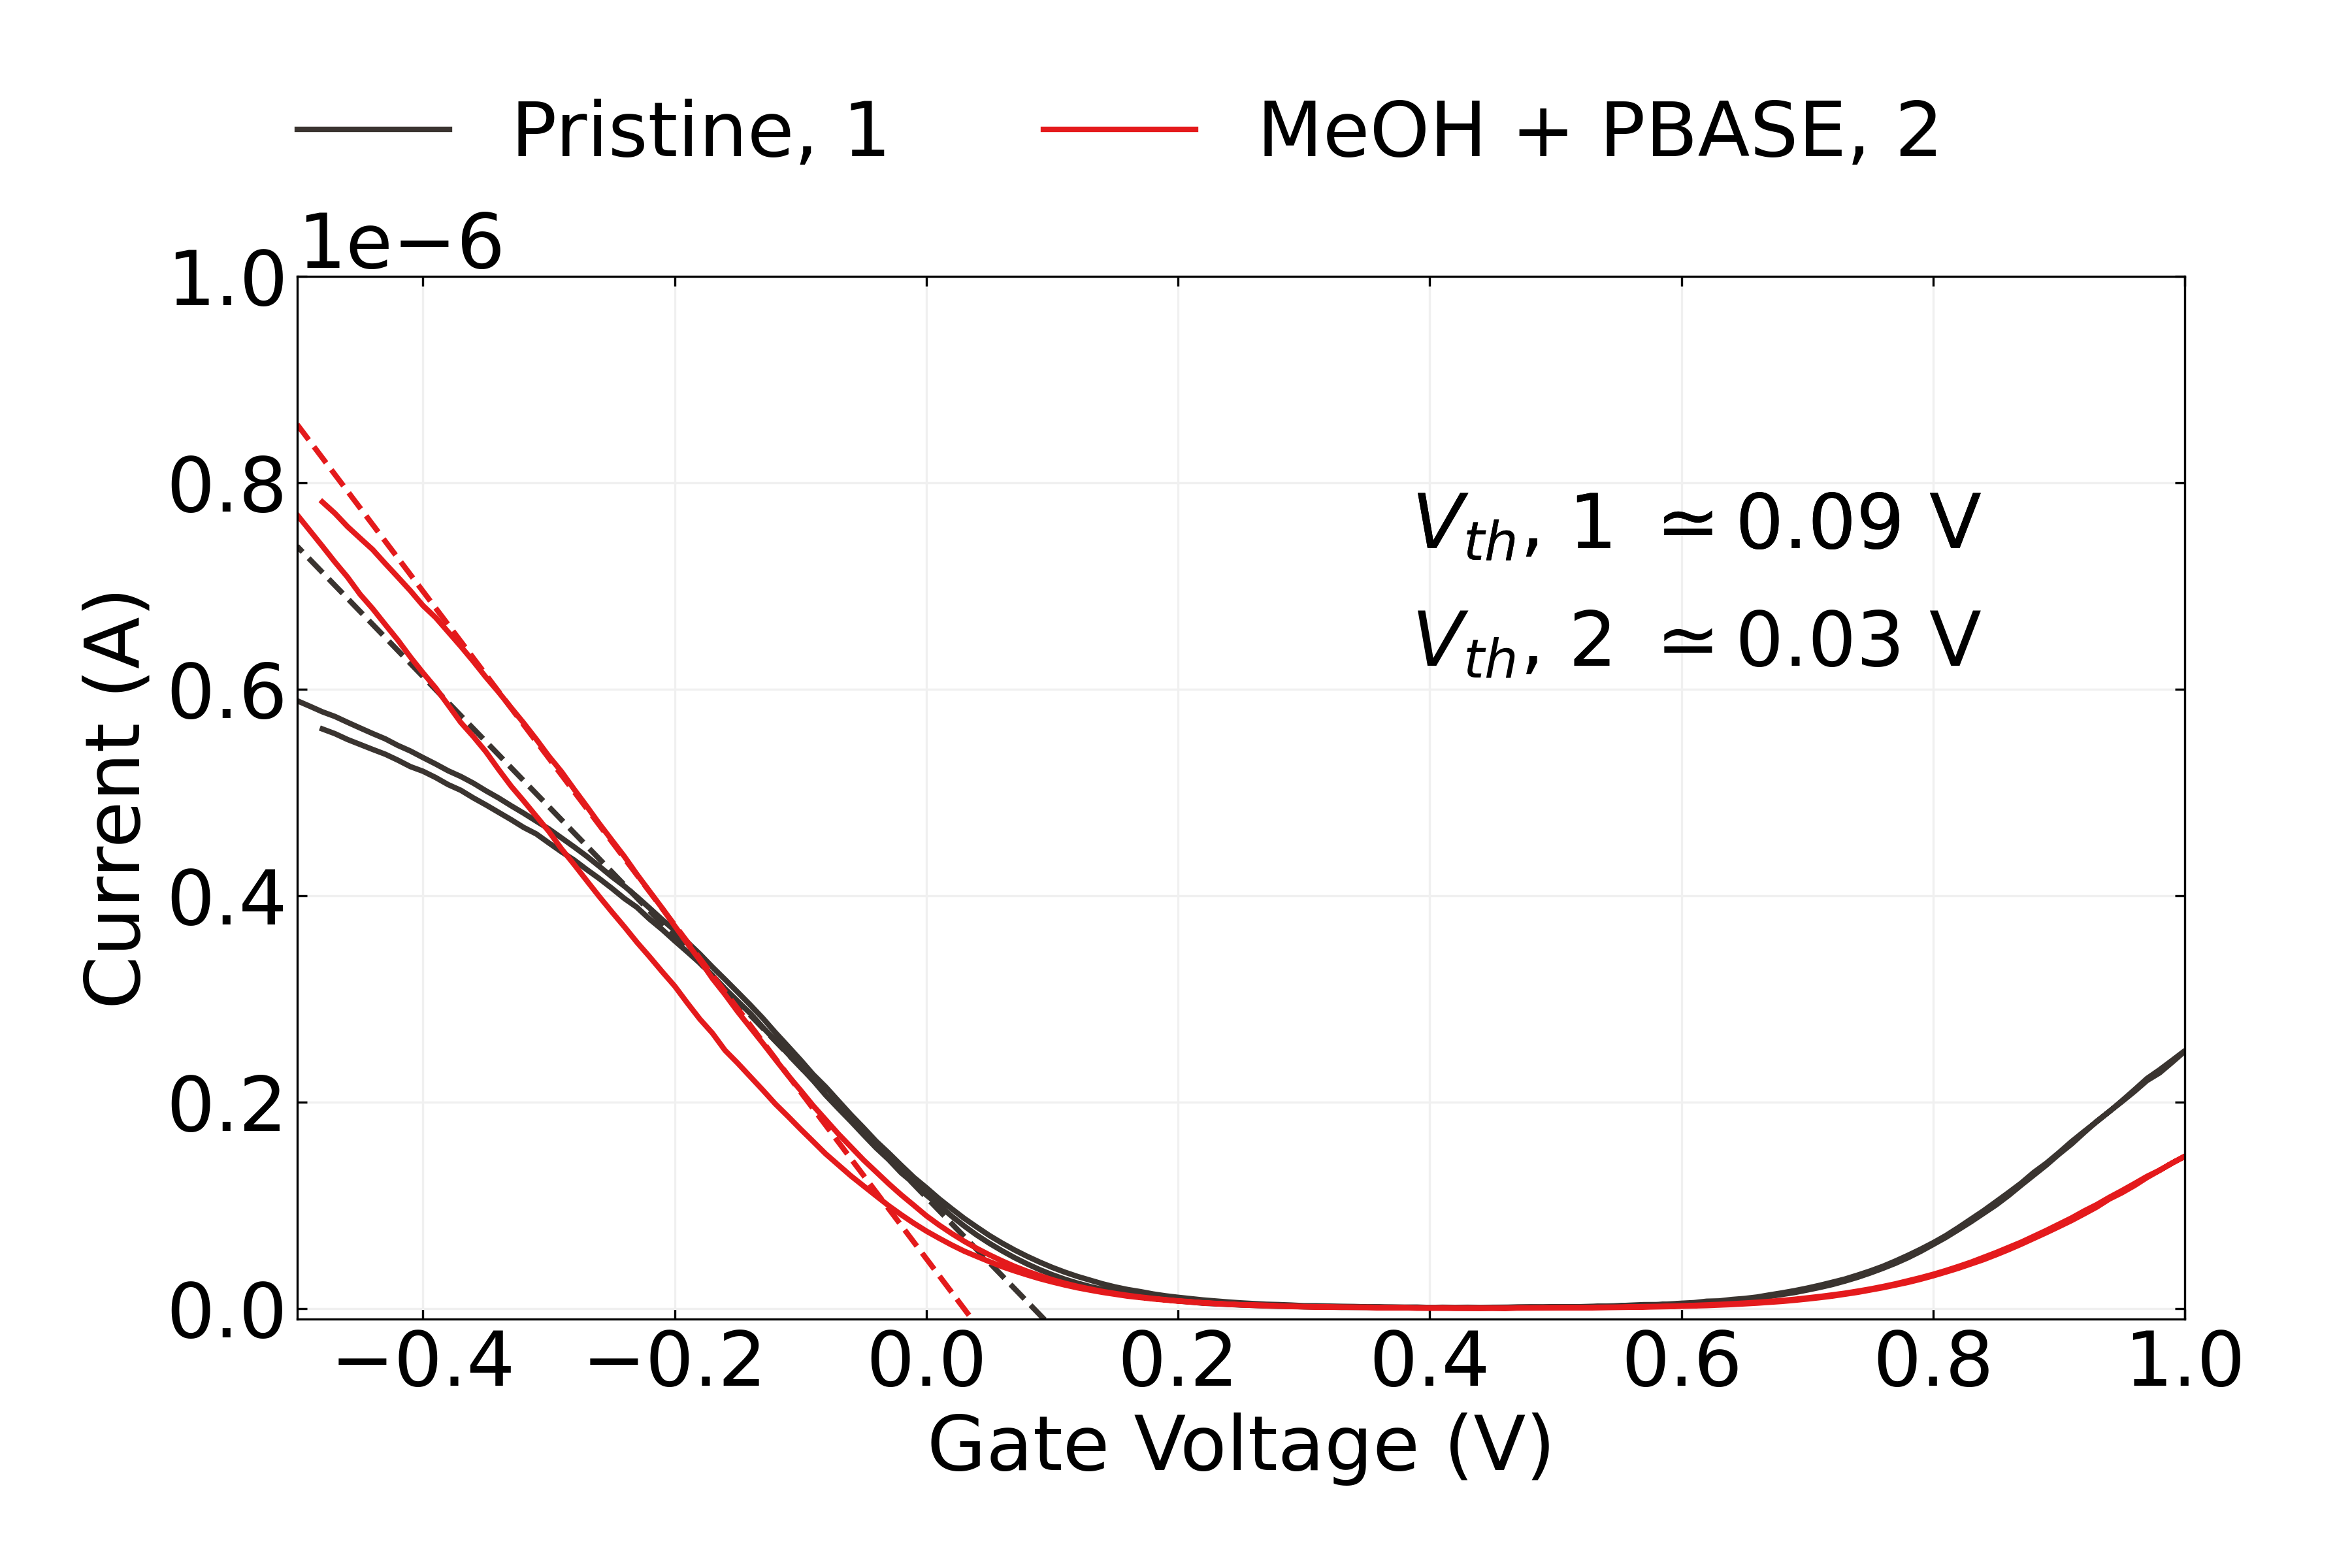
\includegraphics{figures/ch6/Q2C6_ch2_MeOHPBASE.png}

}

}

\end{minipage}%
%
\begin{minipage}[t]{0.01\linewidth}

{\centering 

~

}

\end{minipage}%
%
\begin{minipage}[t]{0.03\linewidth}

{\centering 

\raisebox{-\height}{


\includegraphics{figures/(d).png}

}

}

\end{minipage}%
%
\begin{minipage}[t]{0.01\linewidth}

{\centering 

~

}

\end{minipage}%
%
\begin{minipage}[t]{0.45\linewidth}

{\centering 

\raisebox{-\height}{

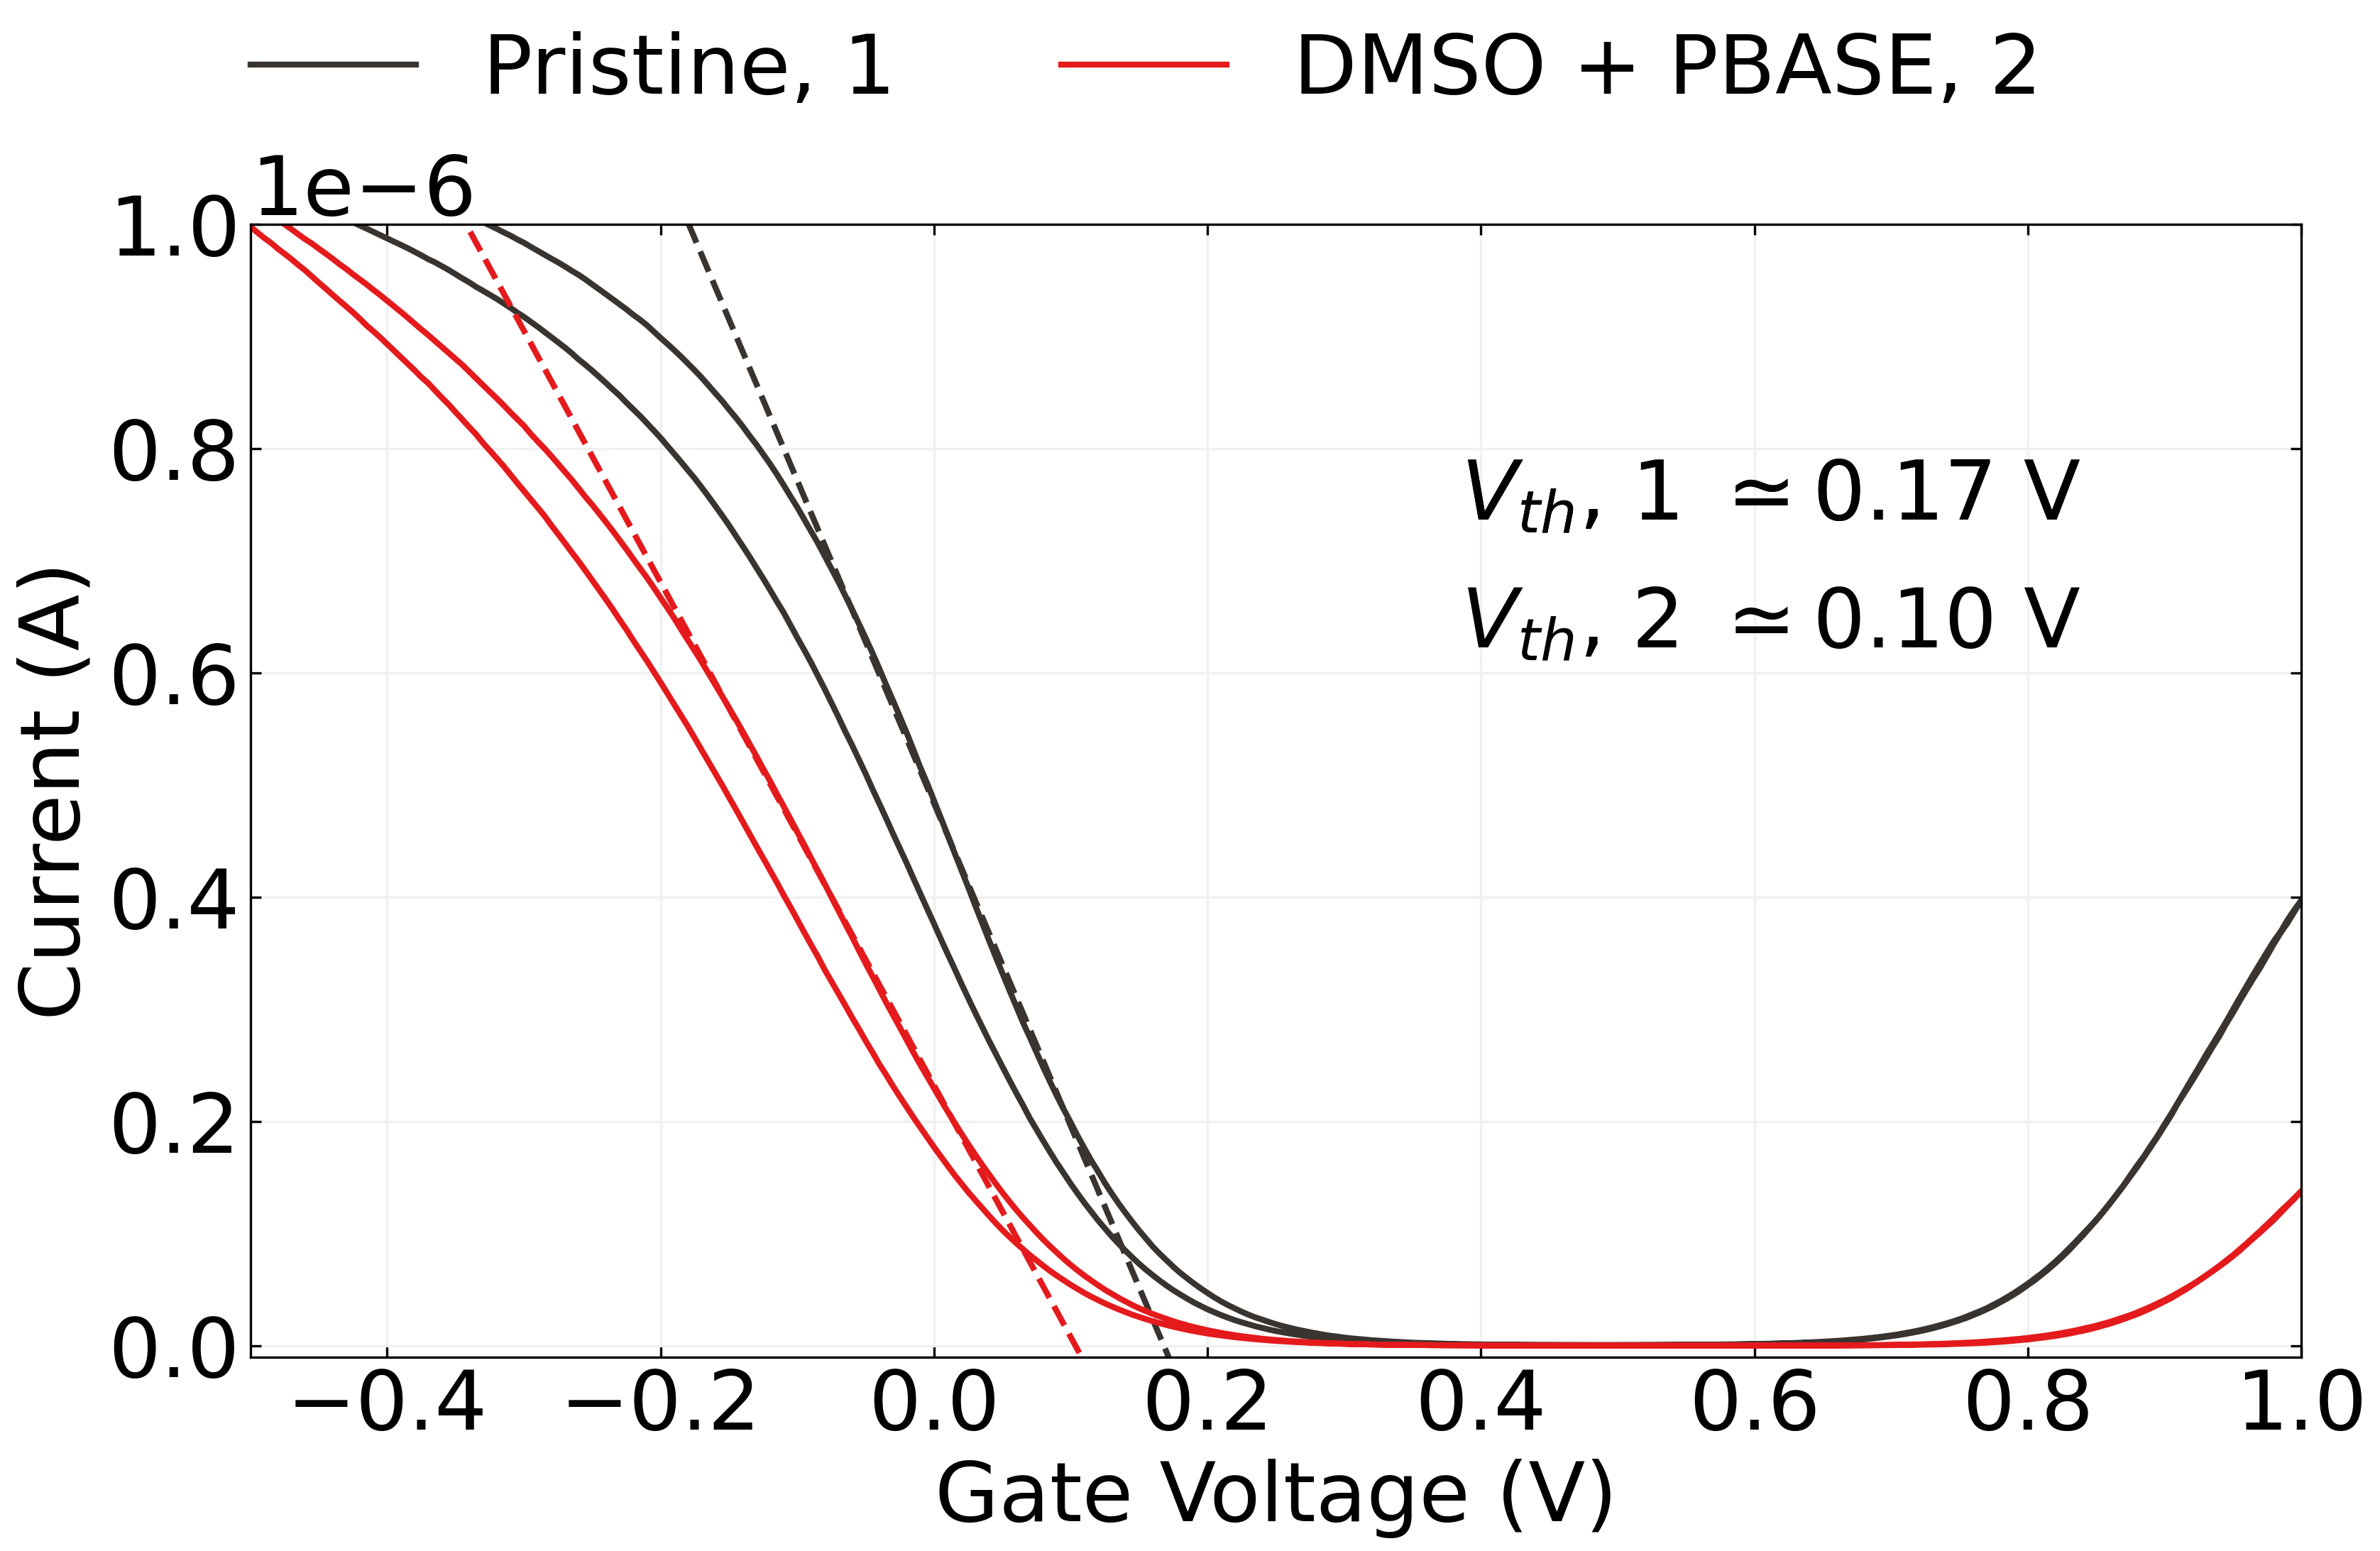
\includegraphics{figures/ch6/Q23D7_ch3_DMSOPBASE.png}

}

}

\end{minipage}%
%
\begin{minipage}[t]{0.01\linewidth}

{\centering 

~

}

\end{minipage}%

\caption[The transfer characteristics of carbon nanotube transistors
before and after being submerged in MeOH or DMSO for one hour, either
with or without 1 mM PBASE
present.]{\label{fig-PBASE-vs-solvent-only}The transfer characteristics
of carbon nanotube transistors (\(V_{ds}\) = 100 mV) before and after
being submerged in MeOH (a) or DMSO (b) for one hour and subsequently
rinsed with deionised water. The change in characteristics of similar
transistor channels after being submerged in these same solvents
containing 1 mM PBASE for one hour and then rinsed are shown in (c) and
(d) respectively. The threshold voltage for the forward sweep of each
transfer characteristic curve is also shown.}

\end{figure}

Capacitive gating results from dense coverage of adsorped molecules on
the carbon nanotube surface which have a low permittivity relative to
the surrounding electrolyte {[}@Heller2008{]}. The relative permittivity
of MeOH and DMSO are \(\sim\) 33 {[}@Mohsen-Nia2010{]} and \(\sim\) 47
{[}@Hunger2010{]} respectively, which are both much lower than the
relative permittivity of PBS, \(\sim\) 80 {[}@Shkodra2021{]}. From
Figure~\ref{fig-PBASE-vs-solvent-only} (a) and
Figure~\ref{fig-PBASE-vs-solvent-only} (b), the threshold shift values
found resulting from exposure to each solvent, taking the average of
forward and reverse sweep values from a single device, were
\(\Delta V = -0.15 \pm 0.02\) V and \(\Delta V = -0.15 \pm 0.01\) V for
MeOH and DMSO respectively. The average threshold shift value for a
second device exposed to MeOH was \(\Delta V = -0.16 \pm 0.02\) V,
indicating that this threshold shift result is reproducible.

Using the same characterisation process as in this work, Murugathas
\emph{et al.} {[}@Murugathas2019a{]} showed that the attachment of PBASE
to a solvent-deposited carbon nanotube network had little effect on
channel threshold voltage, implying the presence of PBASE had not
significantly influenced channel gating. Here, an average threshold
voltage shift of \(-0.06 \pm 0.04\) V is seen after PBASE
functionalisation in MeOH and \(-0.06 \pm 0.01\) V after PBASE
functionalisation in DMSO. These threshold voltage shifts are small
compared to the shift values from solvent exposure. It is possible that
the attachment of PBASE prevents solvent adsorption, and has a small
negative gating effect on the channel. Alternatively, while the solvent
negatively gates the channel, resulting in a threshold shift of
\(-0.15\) V, the PBASE may be counteracting this by positively gating
the channel, resulting in a threshold shift of \(+0.09\) V. Murugathas
\emph{et al.} also observed a slight increase in channel conductance
after PBASE functionalisation {[}@Murugathas2019a{]}.
Figure~\ref{fig-PBASE-vs-solvent-only} also shows a slight increase in
channel conductance post-functionalisation in both
Figure~\ref{fig-PBASE-vs-solvent-only} (c) and
Figure~\ref{fig-PBASE-vs-solvent-only} (d) relative to the solvent-only
case in Figure~\ref{fig-PBASE-vs-solvent-only} (a) and
Figure~\ref{fig-PBASE-vs-solvent-only} (b). This result implies that the
presence of PBASE molecules increases channel mobility and therefore
conductance {[}@Heller2008{]}.

The absorption of organic solvent by the carbon nanotube network has
unknown but potentially negative implications for biosensor
functionalisation. Use of organic solvents in functionalisation can also
attack the encapsulation layer of devices, promoting gate current
leakage. In light of these issues, recent work has begun to explore
alternative aqueous-based methods for functionalisation of biosensors
{[}@Khan2021{]}. The discussion here also illustrates the importance of
considering each substance used when characterising a device to verify
if functionalisation has worked. The qualitative presence of a change in
characteristics (or lack of one) over the full process is not sufficient
to make conclusive remarks regarding successful functionalisation. A
full set of control measurements are required for an understanding of
electronic changes occurring during the functionalisation process, in
the manner of Besteman \emph{et al.} {[}@Besteman2003{]}.

\hypertarget{sec-PBA}{%
\subsection{Attachment of 1-Pyrenebutyric Acid}\label{sec-PBA}}

\hypertarget{comparing-attachment-methods}{%
\subsubsection{Comparing Attachment
Methods}\label{comparing-attachment-methods}}

Another linker molecule that can be used to attach receptor molecules to
a carbon nanotube or graphene channel is 1-pyrenebutyric acid (PBA or
PyBA). The pyrene group in PBA also undergoes pi-stacking with the
channel surface. PBA can be reacted with
1-ethyl-3-(3-dimethylaminopropyl) carbodiimide hydrochloride (EDC or
EDAC) to form an \emph{O}-acylisourea intermediate, which then reacts
with an amine group on a biomolecule to form an amide or imide bond
{[}@Sehgal1994; @Hermanson2013-4{]}. The water solubility of EDC means
that, unlike PBASE, it is possible to functionalise with EDC dissolved
in water rather than in an organic solvent. However, like PBASE, EDC and
the \emph{O}-acylisourea intermediate are prone to hydrolysis,
especially in acidic conditions. Therefore, like PBASE, it should be
stored at \(-20\) °C, and warmed to room temperature to prevent
condensation build-up, since exposure to condensation will hydrolyse the
reagent {[}@Hermanson2013-4{]}. Furthermore, by adding
N-hydroxysuccinimide (NHS) or N-hydroxysulfosuccinimide (Sulfo-NHS or
NHSS) to the reaction vessel, PBASE is formed as an active intermediate,
which is less prone to hydrolysis and increases the PBA/EDC reaction
yield {[}@Sehgal1994; @Hermanson2013-4; @Hermanson2013-14{]}.

To the best of my knowledge, a full comparison of functionalisation
procedures used for linking carbon nanotube and graphene devices to
aptamers and proteins with PBA is given in
Table~\ref{tbl-pba-functionalisation}. By comparing
\textbf{?@tbl-pbase-functionalisation} and
Table~\ref{tbl-pba-functionalisation}, it is clear that PBASE is more
widely used for non-covalent functionalisation than PBA/EDC. As with
PBASE, there are a wide range of process variables used for the PBA
functionalisation process. Also notable is the frequent use of
polyethylene glycol (PEG) or pyrene-PEG for prevention of non-specific
binding (see \textbf{?@sec-non-specific-binding} for a further
discussion of NSB). Despite being less widely used, Mishyn \emph{et al.}
{[}@Mishyn2022{]} state a preference for the use of PBA/EDC over PBASE,
as they found it gave a larger reaction yield when binding ferrocene to
graphene. A potential downside of using PBA/EDC for protein
immobilisation is that EDC has numerous ways of interacting with
proteins, and not all of these are necessarily desirable. Furthermore,
the addition of NHS may cause other issues, such as precipitation of the
reaction compound {[}@Hermanson2013-4{]}. The greater range of process
variables involved in the functionalisation also makes reproducing past
results more complex.

\hypertarget{raman-spectroscopy}{%
\subsubsection{Raman Spectroscopy}\label{raman-spectroscopy}}

Raman spectroscopy was used to verify the attachment of PBA to a carbon
nanotube network film with a SiO\(_2\) substrate in the manner outlined
in \textbf{?@sec-raman-characterisation}. As highly bundled devices were
found to have fewer defects present prior to modification, as discussed
in \textbf{?@sec-pristine-raman}, solvent-deposited films were used for
the verification of pyrene attachment to prevent the initial presence of
defects influencing the analysis.

\newgeometry{a4paper,centering=true,right=1.5in,headsep=44.95pt,footskip=23pt}
\begin{landscape}
\begin{center}

\begin{Shaded}
\begin{Highlighting}[]
\NormalTok{knitr}\SpecialCharTok{::}\NormalTok{opts\_chunk}\SpecialCharTok{$}\FunctionTok{set}\NormalTok{(}\AttributeTok{echo =} \ConstantTok{FALSE}\NormalTok{)}
\FunctionTok{library}\NormalTok{(knitr)}

\NormalTok{pba\_table }\OtherTok{\textless{}{-}} \FunctionTok{read.csv}\NormalTok{(}\StringTok{"tables/ch6/pba\_table.csv"}\NormalTok{, }\AttributeTok{sep=}\StringTok{","}\NormalTok{)}
\NormalTok{pba\_table }\OtherTok{\textless{}{-}}\NormalTok{ pba\_table[}\FunctionTok{rowSums}\NormalTok{(}\FunctionTok{is.na}\NormalTok{(pba\_table)) }\SpecialCharTok{==} \DecValTok{0}\NormalTok{,]}

\NormalTok{knitr}\SpecialCharTok{::}\FunctionTok{kable}\NormalTok{(pba\_table, }
            \AttributeTok{col.names =} \FunctionTok{c}\NormalTok{(}\StringTok{"Solvent"}\NormalTok{,}
                           \StringTok{"Channel"}\NormalTok{,}
                           \StringTok{"PBA (mM)"}\NormalTok{,}
                           \StringTok{"Time (hr)"}\NormalTok{,}
                           \StringTok{"EDC (mM)"}\NormalTok{,}
                           \StringTok{"NHS (mM)"}\NormalTok{,}
                           \StringTok{"NHSS (mM)"}\NormalTok{,}
                           \StringTok{"Time (min)"}\NormalTok{,}
                           \StringTok{"References"}\NormalTok{),}
            \AttributeTok{column\_spec =} \FunctionTok{c}\NormalTok{(}\FunctionTok{rep}\NormalTok{(}\ConstantTok{NULL}\NormalTok{, }\DecValTok{2}\NormalTok{), }\StringTok{"border{-}left: 2px solid black"}\NormalTok{),}
            \AttributeTok{format =} \StringTok{"simple"}\NormalTok{)}
\end{Highlighting}
\end{Shaded}

\hypertarget{tbl-pba-functionalisation}{}
\begin{longtable}[]{@{}lllllllll@{}}
\caption{\label{tbl-pba-functionalisation}Comparison of 1-pyrenebutyric
acid (PBA) functionalisation processes.
1-ethyl-3-(3-dimethylaminopropyl) carbodiimide hydrochloride (EDC) and
NHS or NHSS (N-hydroxysulfosuccinimide) were co-mingled with PBA during
each process. Device exposure times to each compound are shown next to
the compound concentration. Blank entries indicate there was no mention
of the parameter in a particular paper. \(^†\)PEG or PEG pyrene were
used to reduce non-specific binding. \(^{††}\)Several pyrene-based
linkers were compared and PBA gave an optimal functionalisation
result.}\tabularnewline
\toprule\noalign{}
Solvent & Channel & PBA (mM) & Time (hr) & EDC (mM) & NHS (mM) & NHSS
(mM) & Time (min) & References \\
\midrule\noalign{}
\endfirsthead
\toprule\noalign{}
Solvent & Channel & PBA (mM) & Time (hr) & EDC (mM) & NHS (mM) & NHSS
(mM) & Time (min) & References \\
\midrule\noalign{}
\endhead
\bottomrule\noalign{}
\endlastfoot
DMF & Graphene & 0.6 & 1 & - & - & - & 120 & Gao, 2016\(^†\).
\cite{Gao2016} \\
& & 5 & 2 & 2 & 5 & - & 30 & Mishyn, 2022. \cite{Mishyn2022} \\
& CNT & 100 & 3 & 200 & - & - & 30 & Min, 2012. \cite{Min2012} \\
& & 7.6 & 2 & 8 & 20 & - & 120 & Xu, 2014. \cite{Xu2014} \\
DI water & CNT & - & - & 32 & - & 12 & Overnight & Pacios, 2012\(^†\).
\cite{Pacios2012} \\
Ethanol & CNT & 1 & 1 & 100 & 100 & - & 20 & Filipiak, 2018\(^†\).
\cite{Filipiak2018} \\
Acetonitrile & Graphene & 1 & 1 & 400 & 100 & - & 60 & Tong,
2020\(^{††}\). \cite{Tong2020} \\
Borax & CNT & 2 & 24 & 2.5 & - & - & 1080 & Liu, 2011\(^†\).
\cite{Liu2011} \\
DMSO & Graphene & 5 & 1 & 50 & 50 & - & 90 & Fenzl, 2017.
\cite{Fenzl2017} \\
\end{longtable}

\end{center}
\end{landscape}
\restoregeometry % Restore the global document page margins

Droplets of DMSO solution were placed on three (solvent-deposited)
carbon nanotube films taken from the same wafer. The DMSO solution on
one film contained 5 mM PBA, the solution on another film contained 5 mM
PBASE, and the DMSO on the final film contained no linker molecule.
After incubation for 1 hour, films were rinsed for 15 s with DMSO, then
for 15 s with IPA to remove excess DMSO while avoiding hydrolysis of the
PBASE. After the first set of Raman spectra was taken, the film
initially exposed to PBA was further exposed to a solution of 20 mM EDC
and 40 mM NHS in \(1 \times\) phosphate buffer saline (PBS) electrolyte
for 30 minutes, and a second set of Raman spectra was taken for this
film. As in \textbf{?@sec-pristine-raman}, two spectra taken at each
position were processed according to \textbf{?@sec-raman-analysis}, and
the SiO\(_2\) reference peak measured in the wavenumber range 100
cm\(^{-1}\) \(-\) 650 cm\(^{-1}\) was used to normalise the D-band and
G-band peaks from the wavenumber range 1300 cm\(^{-1}\) \(-\) 1650
cm\(^{-1}\). The ratio between the average intensity of the D-peak and
the G\(^+\)-peak at each position was calculated, and the distribution
of ratio values corresponding to each modified film is shown in
Figure~\ref{fig-linker-raman}.

\begin{figure}

{\centering 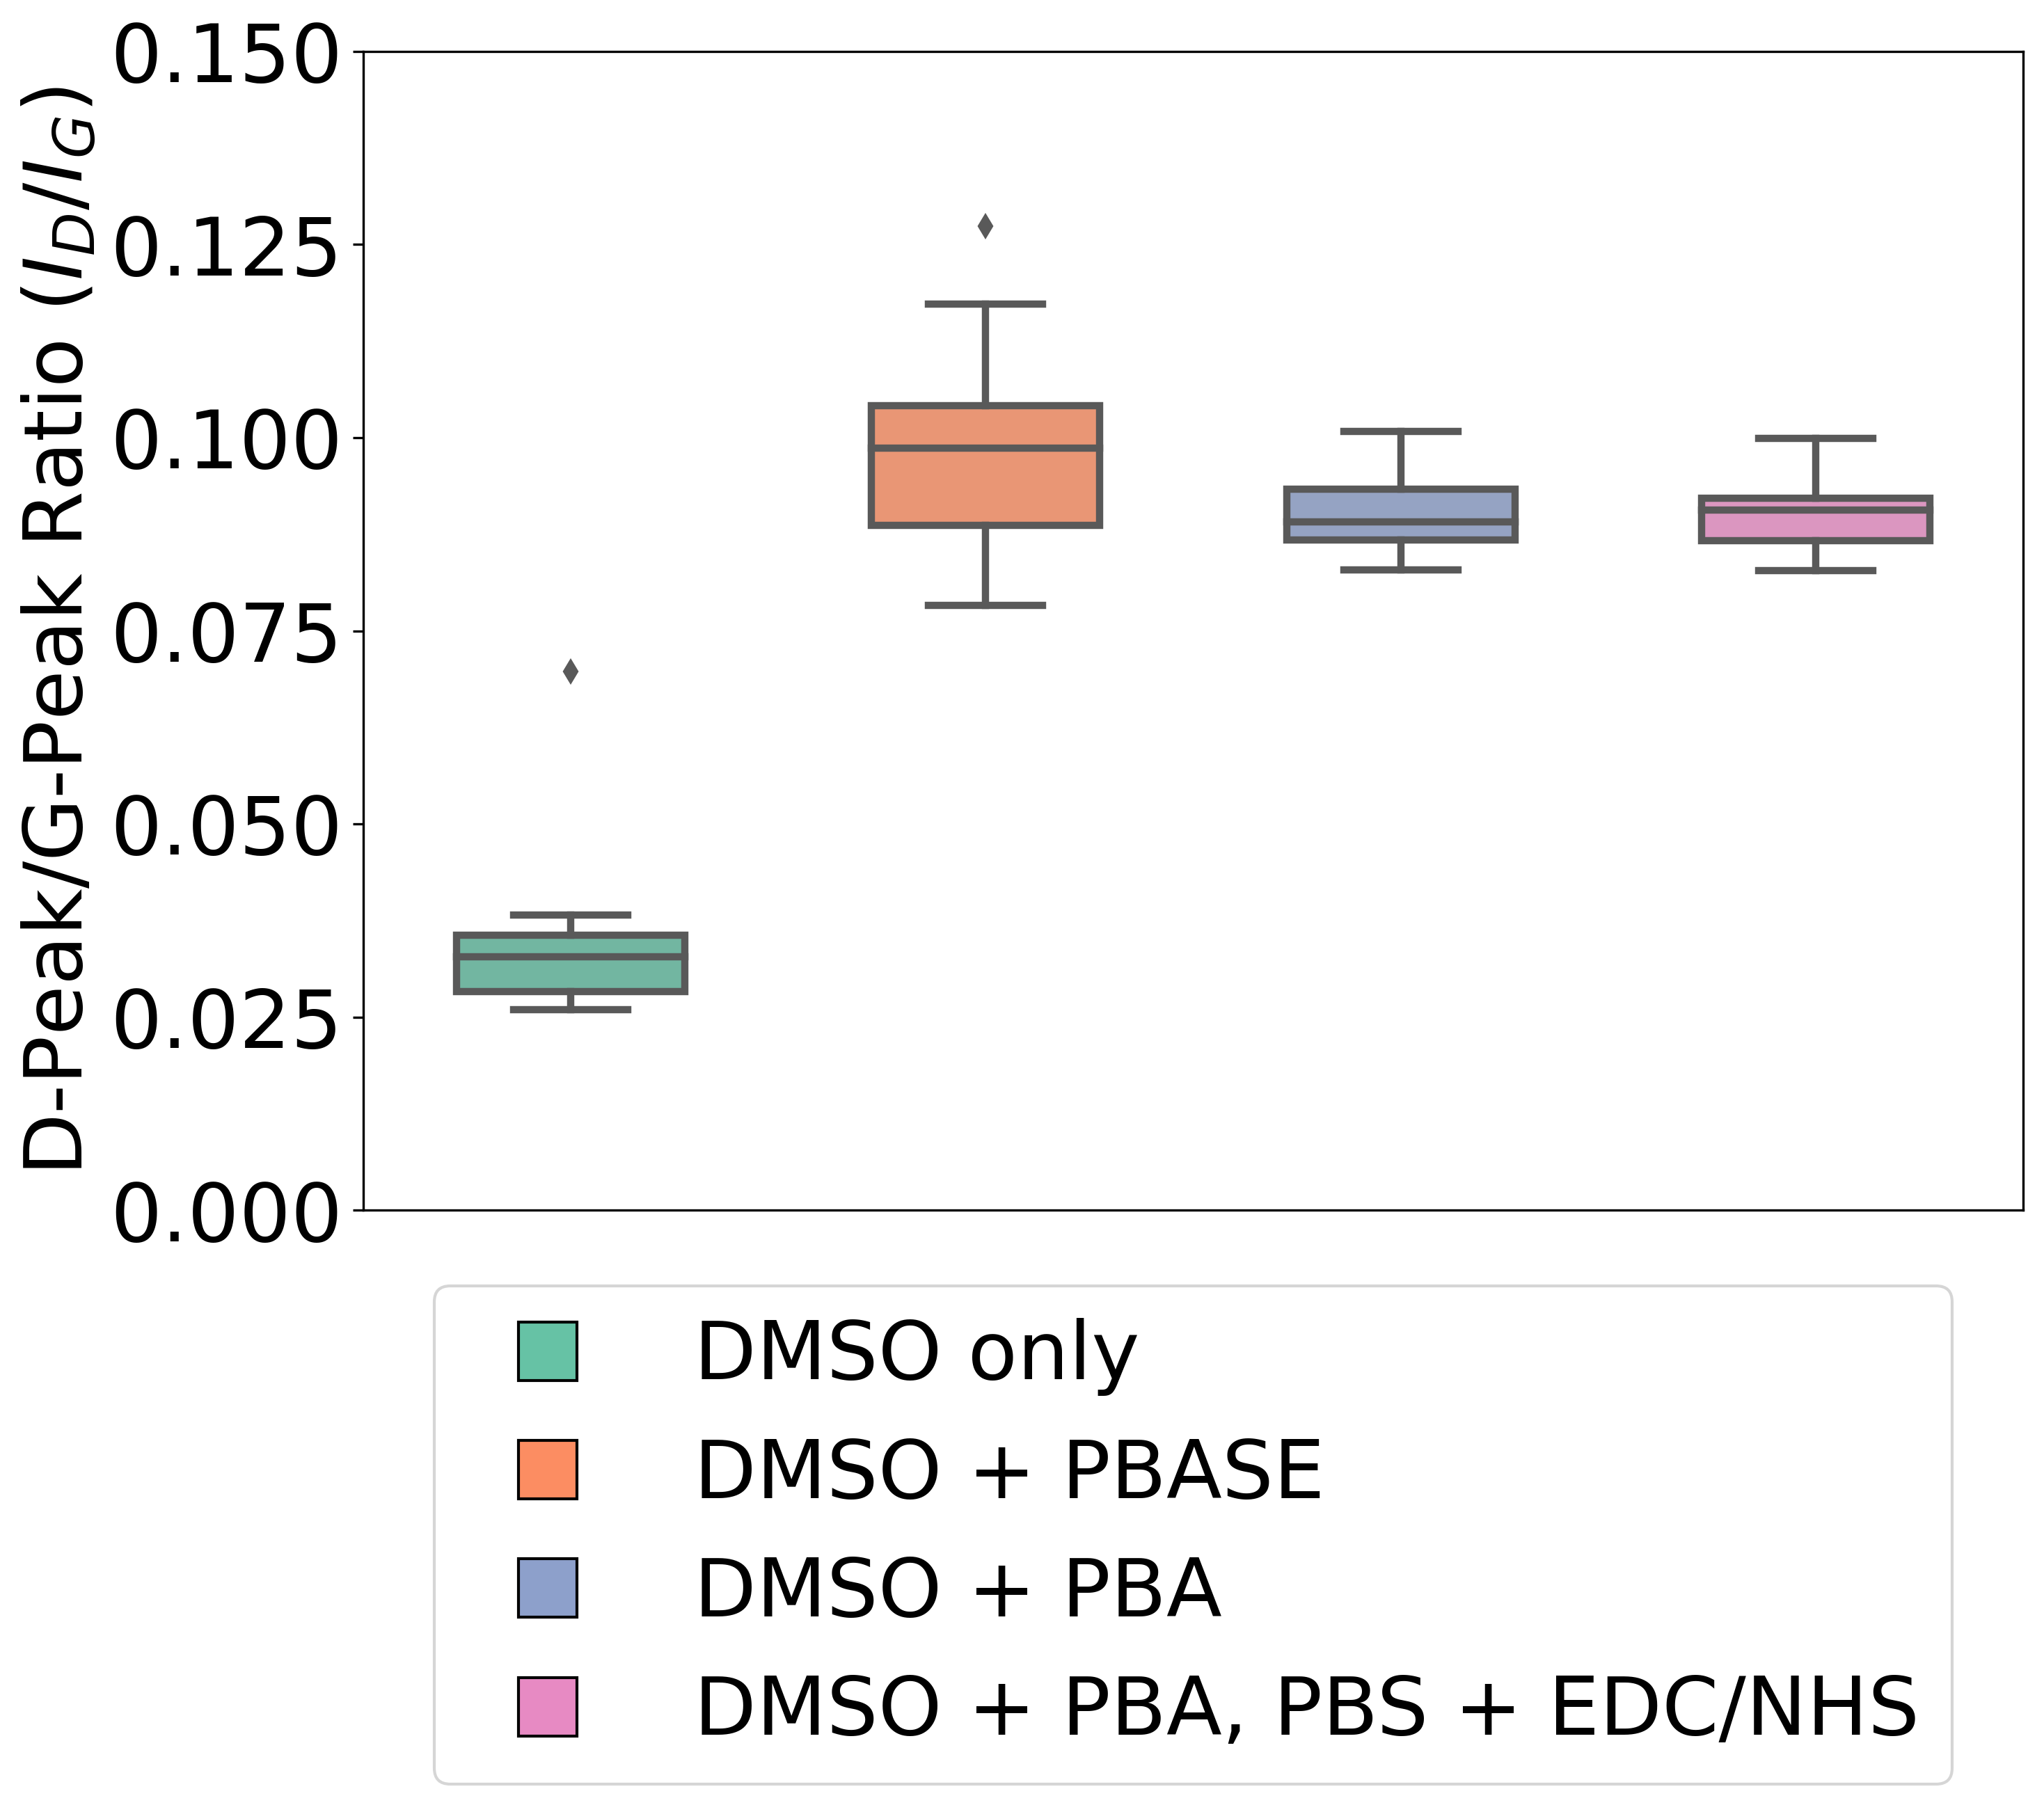
\includegraphics[width=0.5\textwidth,height=\textheight]{figures/ch6/comparison_raman.png}

}

\caption[A box plot showing the distribution of D-band peak to
G\(^+\)-band peak ratios, \(I_D/I_G\), across nine locations for a
selection of chemically-modified carbon nanotube
films.]{\label{fig-linker-raman}A box plot showing the distribution of
D-band peak to G\(^+\)-band peak ratios, \(I_D/I_G\), across nine
locations for a selection of chemically-modified carbon nanotube films.
The D-band and G-band intensities for all samples were first normalised
to the intensity peak corresponding to the SiO\(_2\) substrate.}

\end{figure}

There is a \(\sim 3 \times\) increase in the intensity ratio \(I_D/I_G\)
for both the films modified with PBASE and PBA compared to the film
which was only exposed to DMSO. Previous works have found that a change
in the intensity ratio indicates successful pi-stacking on the carbon
nanotube surface, as it indicates successful surface modification of the
carbon nanotubes {[}@Wei2010; @Lan2013{]}.

Wei \emph{et al.} {[}@Wei2010{]} found functionalisation with PBASE
altered the ratio by a factor of \(\sim 1.5 \times\), while Lan \emph{et
al.} {[}@Lan2013{]} found that functionalisation with PBA altered the
ratio by a factor of \(\sim 0.8 \times\). The reason for the large
difference between results is not immediately clear, but may result from
the significant differences in the pristine composition and morphology
of carbon nanotube networks used in each publication, and differences in
the functionalisation method used. Across all scan locations in
Figure~\ref{fig-linker-raman}, the value found for \(I_D/I_G\) is
consistently \(\sim 0.095\) for both PBA and PBASE. Furthermore,
subsequent Raman measurements of the PBA-modified film after further
functionalisation with EDC/NHS do not show a significant change in
\(I_D/I_G\). These results indicate that presence of the NHS ester has
little effect on the Raman shift, as expected. Raman spectroscopy
therefore cannot be used to distinguish between the presence of PBA and
PBASE on the device surface. However, it is clear that functionalisation
of the carbon nanotube network with both the PBA and PBASE has led to
measurable pi-stacking between the network and the pyrene group attached
to each compound.

\hypertarget{sec-PBA-characterisation}{%
\subsubsection{Electrical
Characterisation}\label{sec-PBA-characterisation}}

Figure~\ref{fig-pba-functionalisation-threshold-shift} shows the
transfer characteristics of a carbon nanotube transistor channel at
various stages of a PBA/EDC functionalisation, where an excess of
N-hydroxysuccinimide (NHS) was added alongside EDC. A solvent-deposited
carbon nanotube film was used for the device. The PBA was dissolved in
DMSO, and the device channels were exposed to this solution for 1 hour.
The change resulting from PBA exposure is shown in
Figure~\ref{fig-pba-functionalisation-threshold-shift} (a). The
threshold shift with the addition of 5 mM PBA in DMSO for 1 hour is
equivalent to the shift seen when only DMSO is added,
\(\Delta V = -0.15\) V. The lack of a significant threshold shift
attributable to the PBA is a result of pyrene having a neutral charge
state. Any contributions from the charged carboxyl group are screened
from the carbon nanotube sidewalls by surrounding water molecules
{[}@Lerner2012{]}. However, as in the case of the addition of PBASE,
there also appears to be an increase in hole mobility, which may be due
to the pyrene groups increasing connectivity within the carbon nanotube
network {[}@Murugathas2019a{]}.

\begin{figure}

\begin{minipage}[t]{0.03\linewidth}

{\centering 

\raisebox{-\height}{


\includegraphics{figures/(a).png}

}

}

\end{minipage}%
%
\begin{minipage}[t]{0.01\linewidth}

{\centering 

~

}

\end{minipage}%
%
\begin{minipage}[t]{0.45\linewidth}

{\centering 

\raisebox{-\height}{

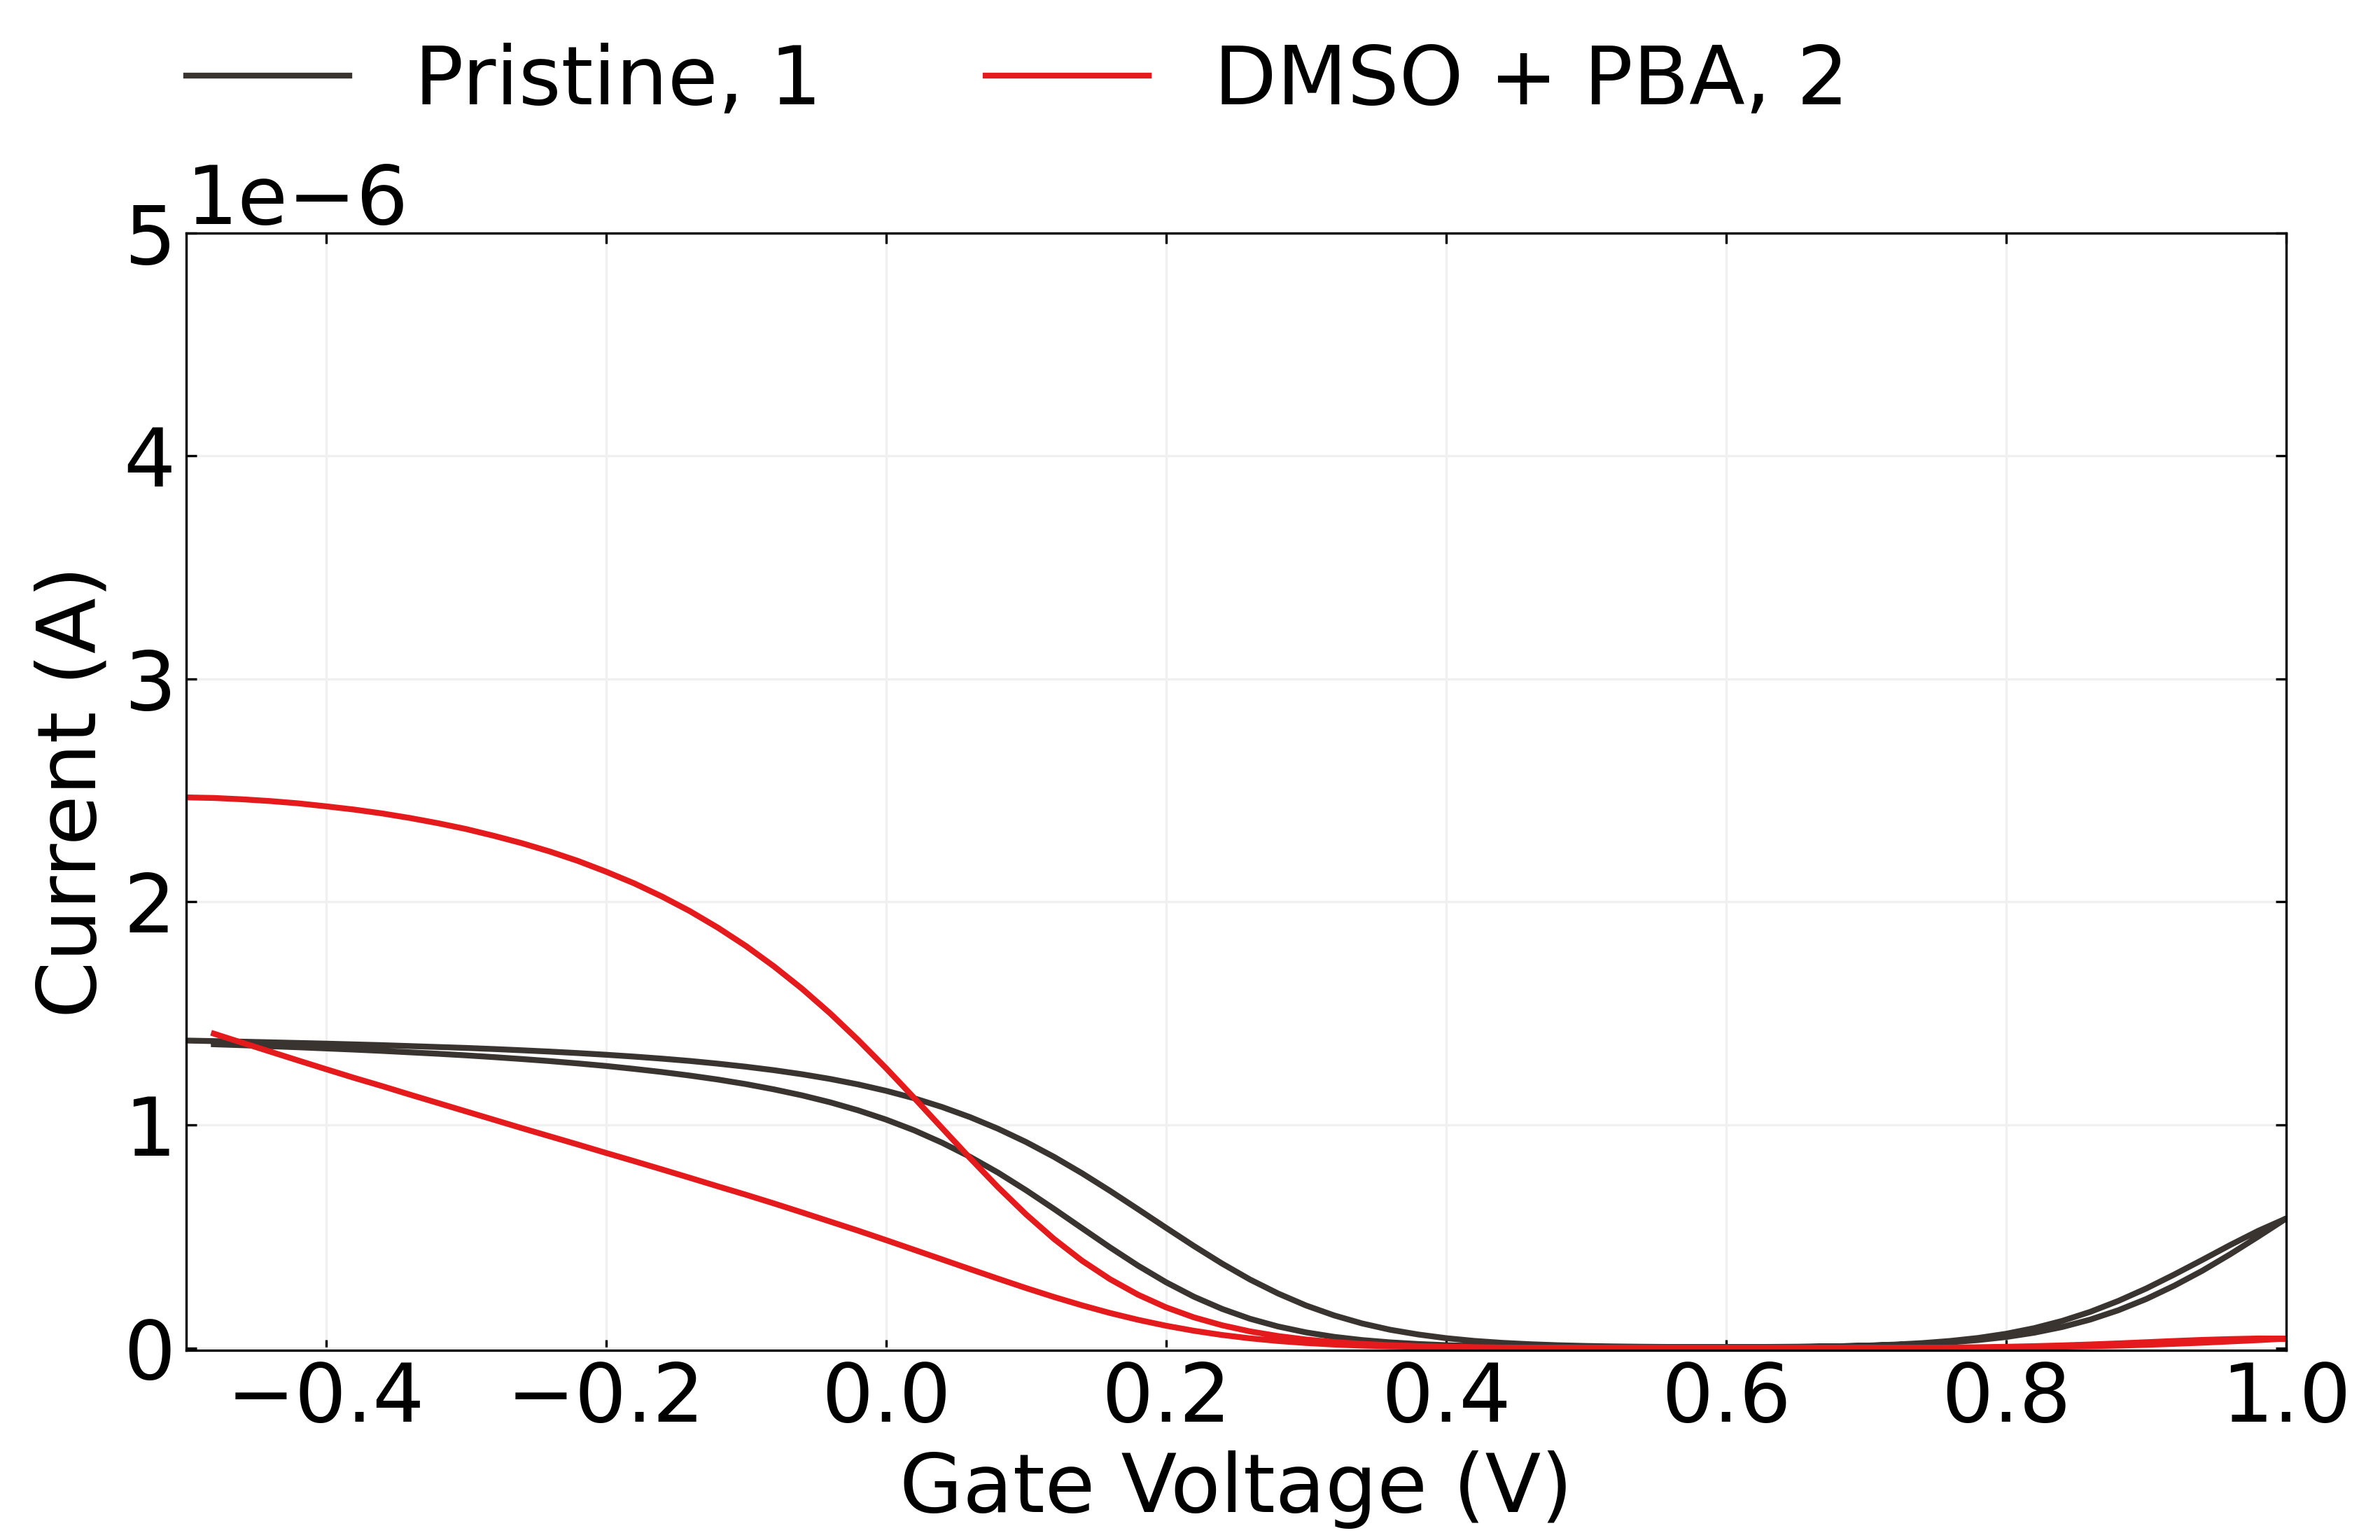
\includegraphics{figures/ch6/NTQ24C10_ch3_comparison_1.png}

}

}

\end{minipage}%
%
\begin{minipage}[t]{0.01\linewidth}

{\centering 

~

}

\end{minipage}%
%
\begin{minipage}[t]{0.03\linewidth}

{\centering 

\raisebox{-\height}{


\includegraphics{figures/(b).png}

}

}

\end{minipage}%
%
\begin{minipage}[t]{0.01\linewidth}

{\centering 

~

}

\end{minipage}%
%
\begin{minipage}[t]{0.45\linewidth}

{\centering 

\raisebox{-\height}{

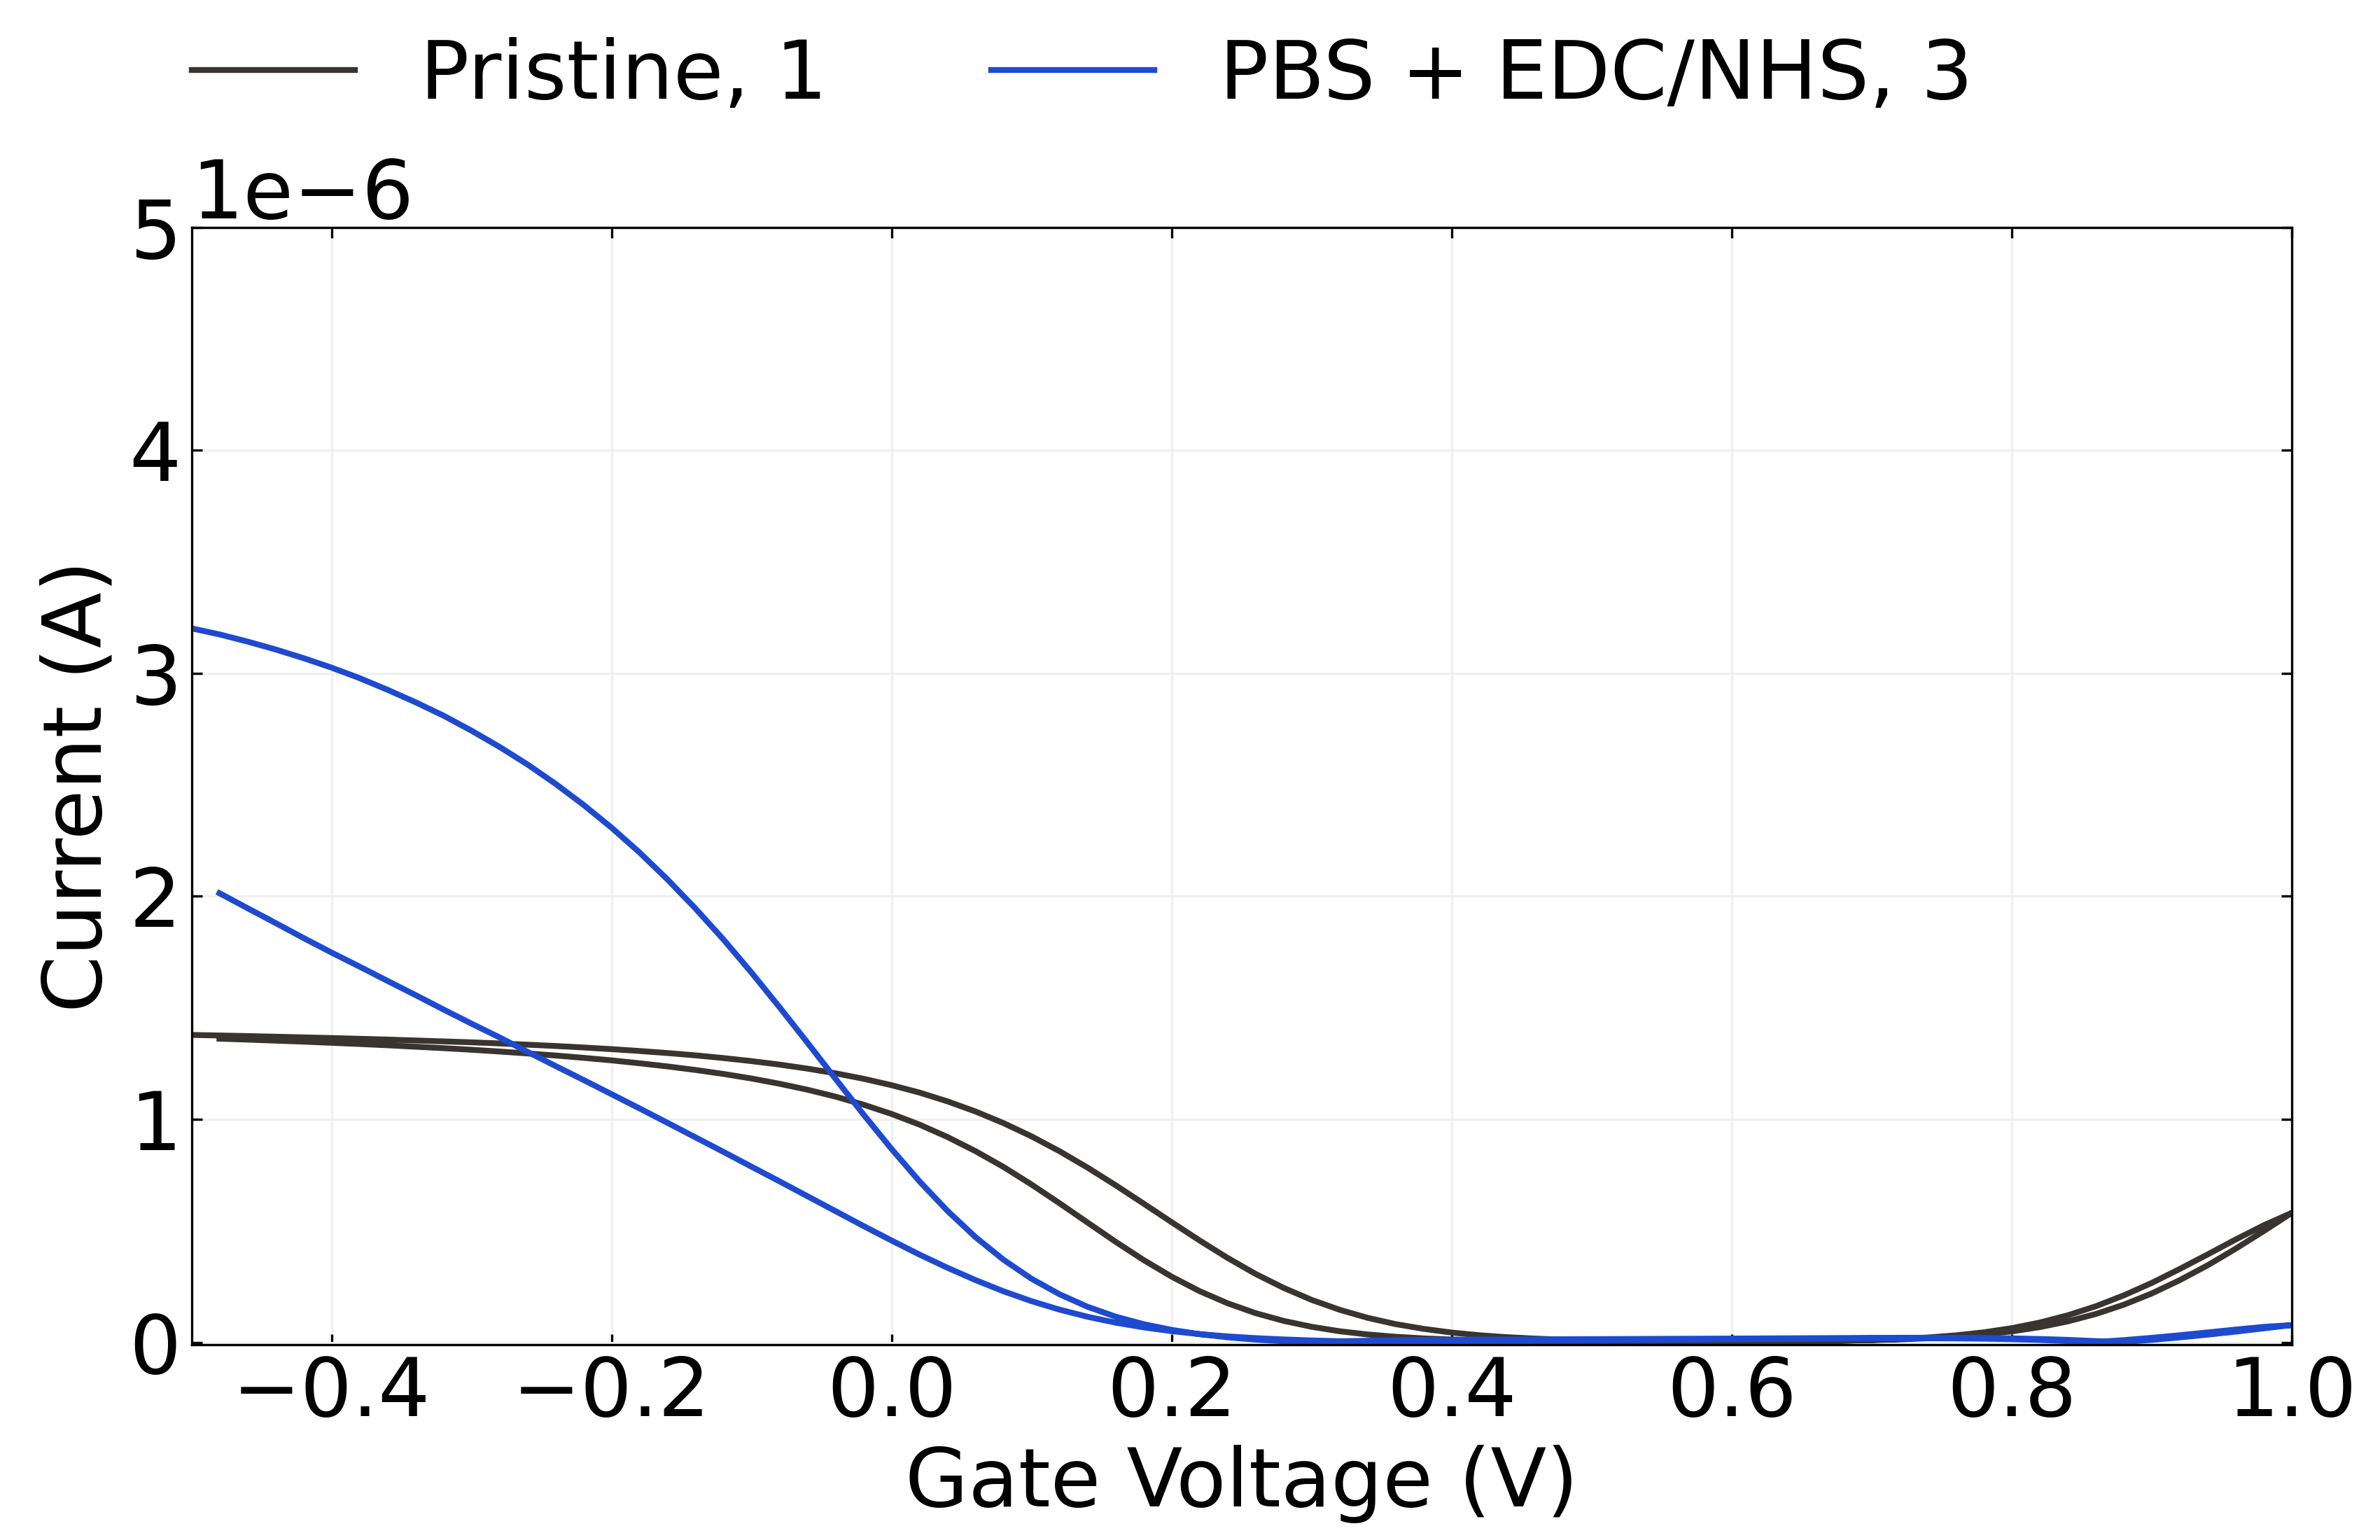
\includegraphics{figures/ch6/NTQ24C10_ch3_comparison_2.png}

}

}

\end{minipage}%
%
\begin{minipage}[t]{0.01\linewidth}

{\centering 

~

}

\end{minipage}%
\newline
\begin{minipage}[t]{0.03\linewidth}

{\centering 

\raisebox{-\height}{


\includegraphics{figures/(c).png}

}

}

\end{minipage}%
%
\begin{minipage}[t]{0.01\linewidth}

{\centering 

~

}

\end{minipage}%
%
\begin{minipage}[t]{0.45\linewidth}

{\centering 

\raisebox{-\height}{

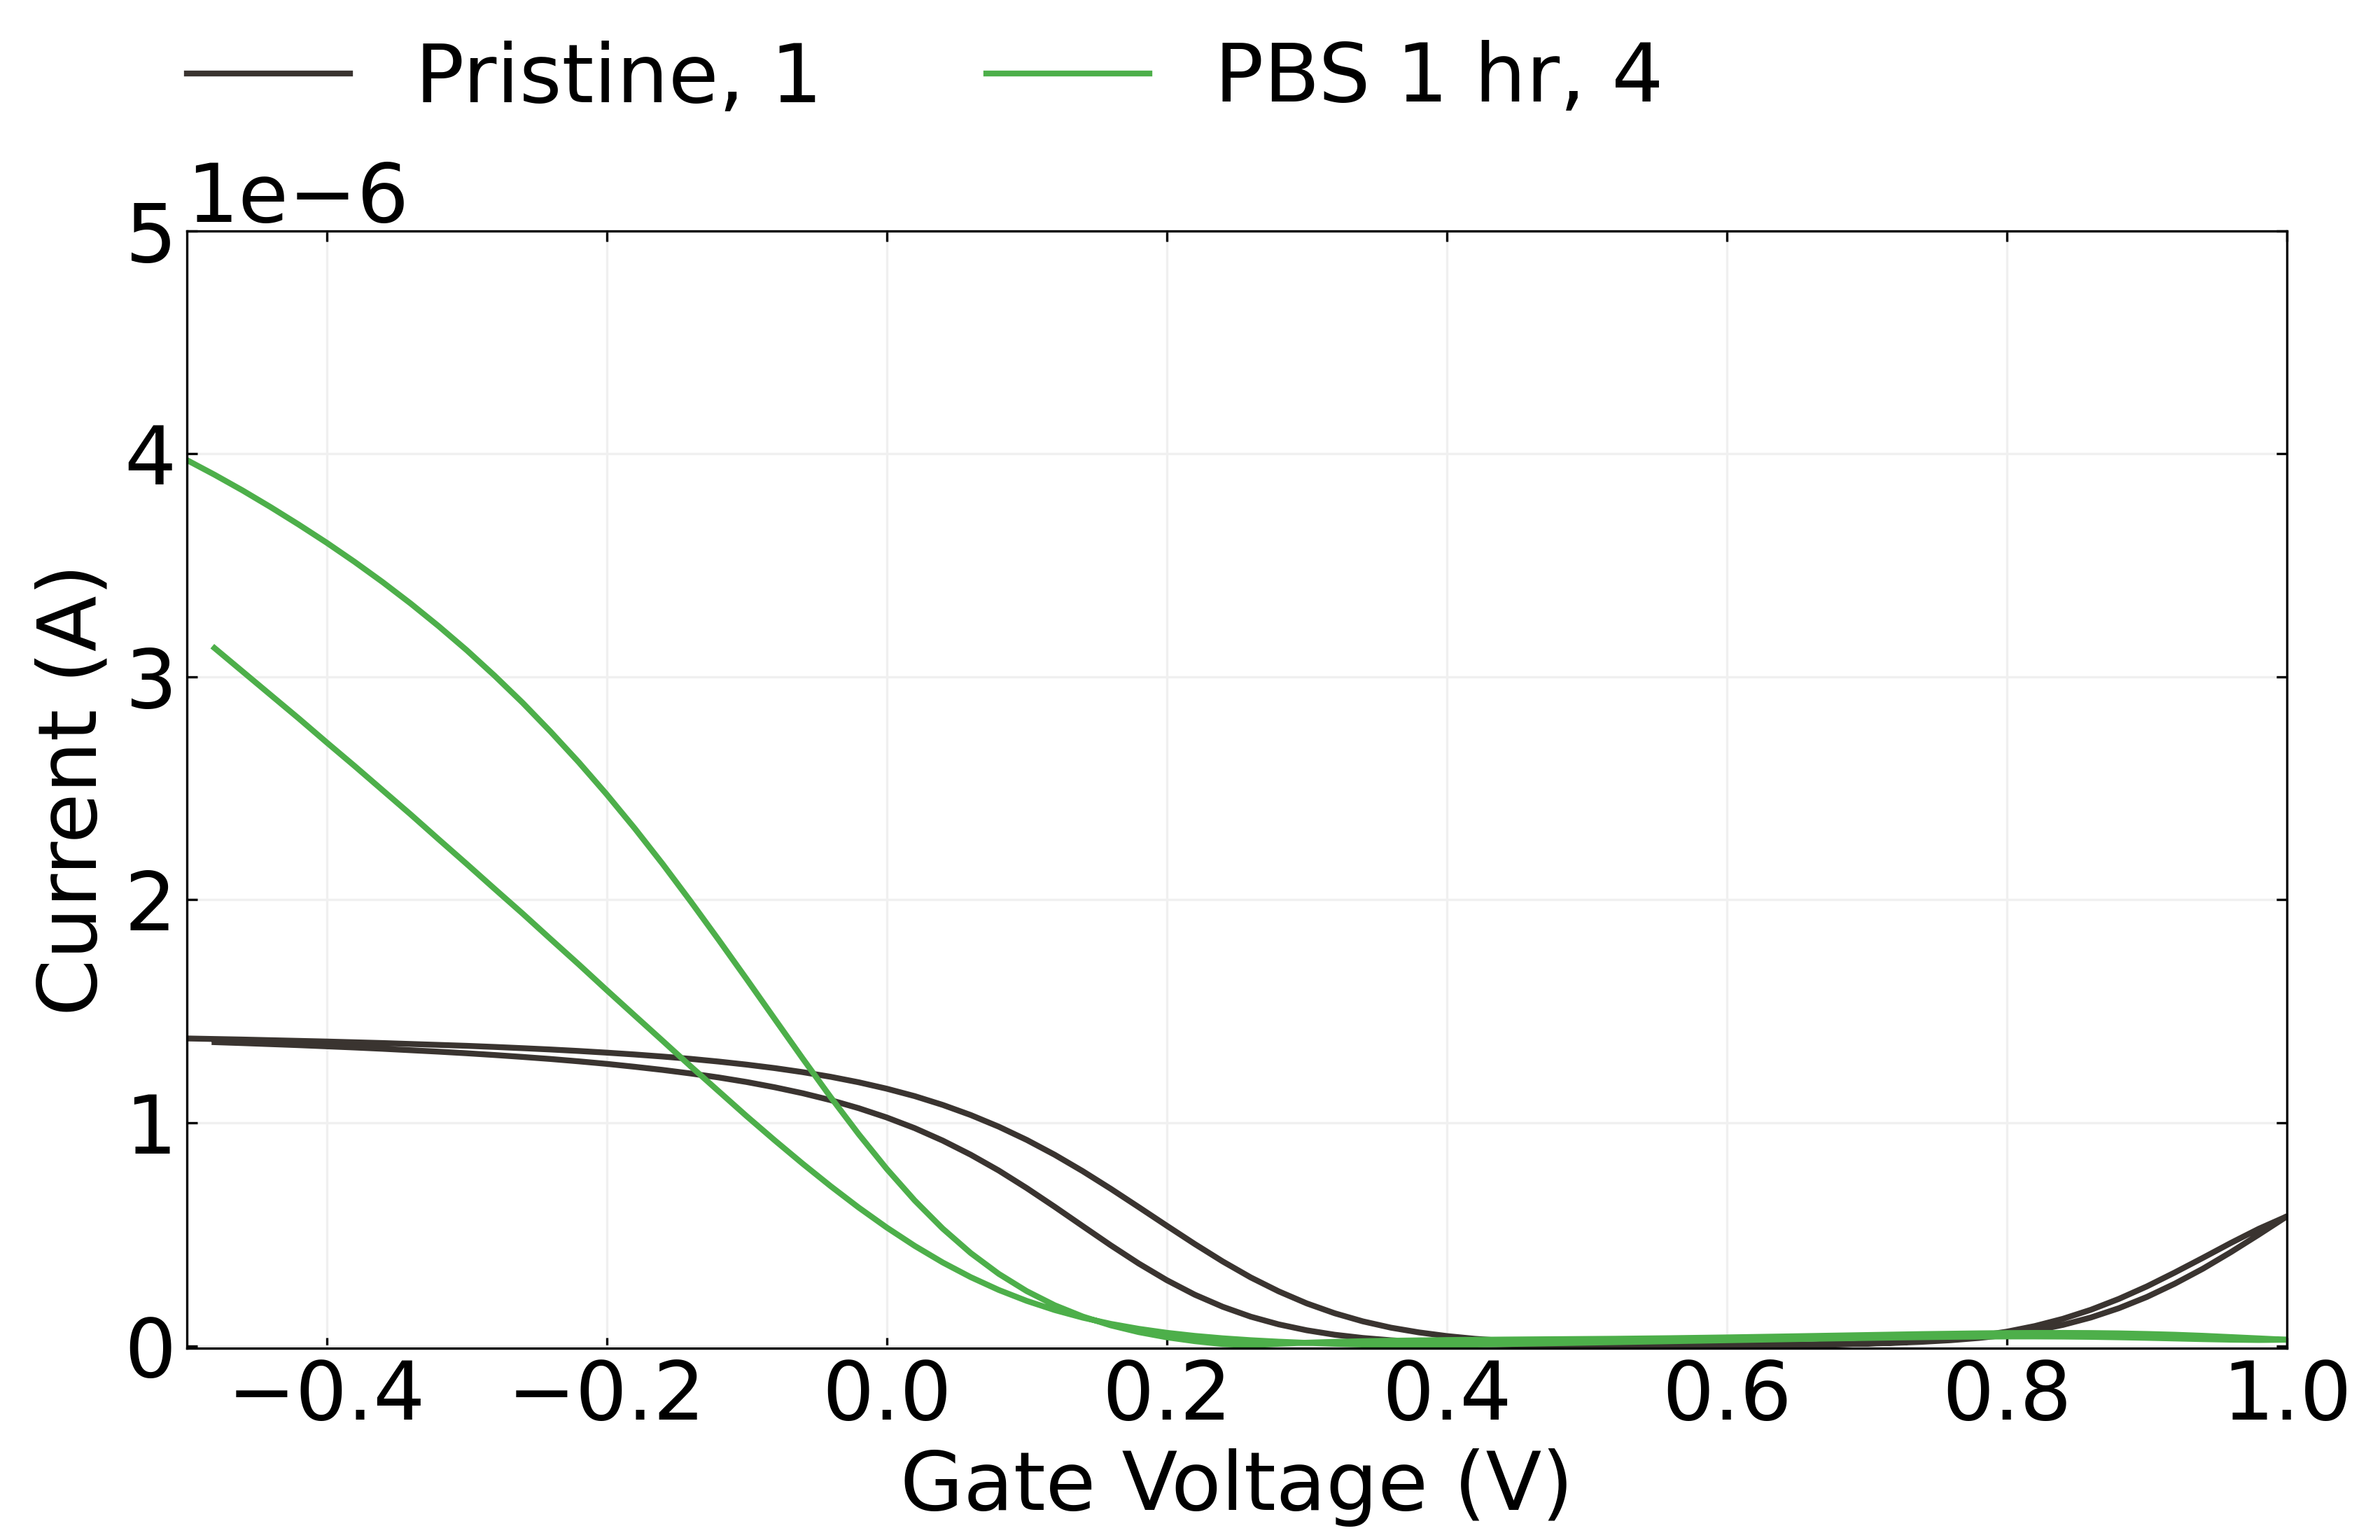
\includegraphics{figures/ch6/NTQ24C10_ch3_comparison_3.png}

}

}

\end{minipage}%
%
\begin{minipage}[t]{0.01\linewidth}

{\centering 

~

}

\end{minipage}%
%
\begin{minipage}[t]{0.03\linewidth}

{\centering 

\raisebox{-\height}{


\includegraphics{figures/(d).png}

}

}

\end{minipage}%
%
\begin{minipage}[t]{0.01\linewidth}

{\centering 

~

}

\end{minipage}%
%
\begin{minipage}[t]{0.45\linewidth}

{\centering 

\raisebox{-\height}{

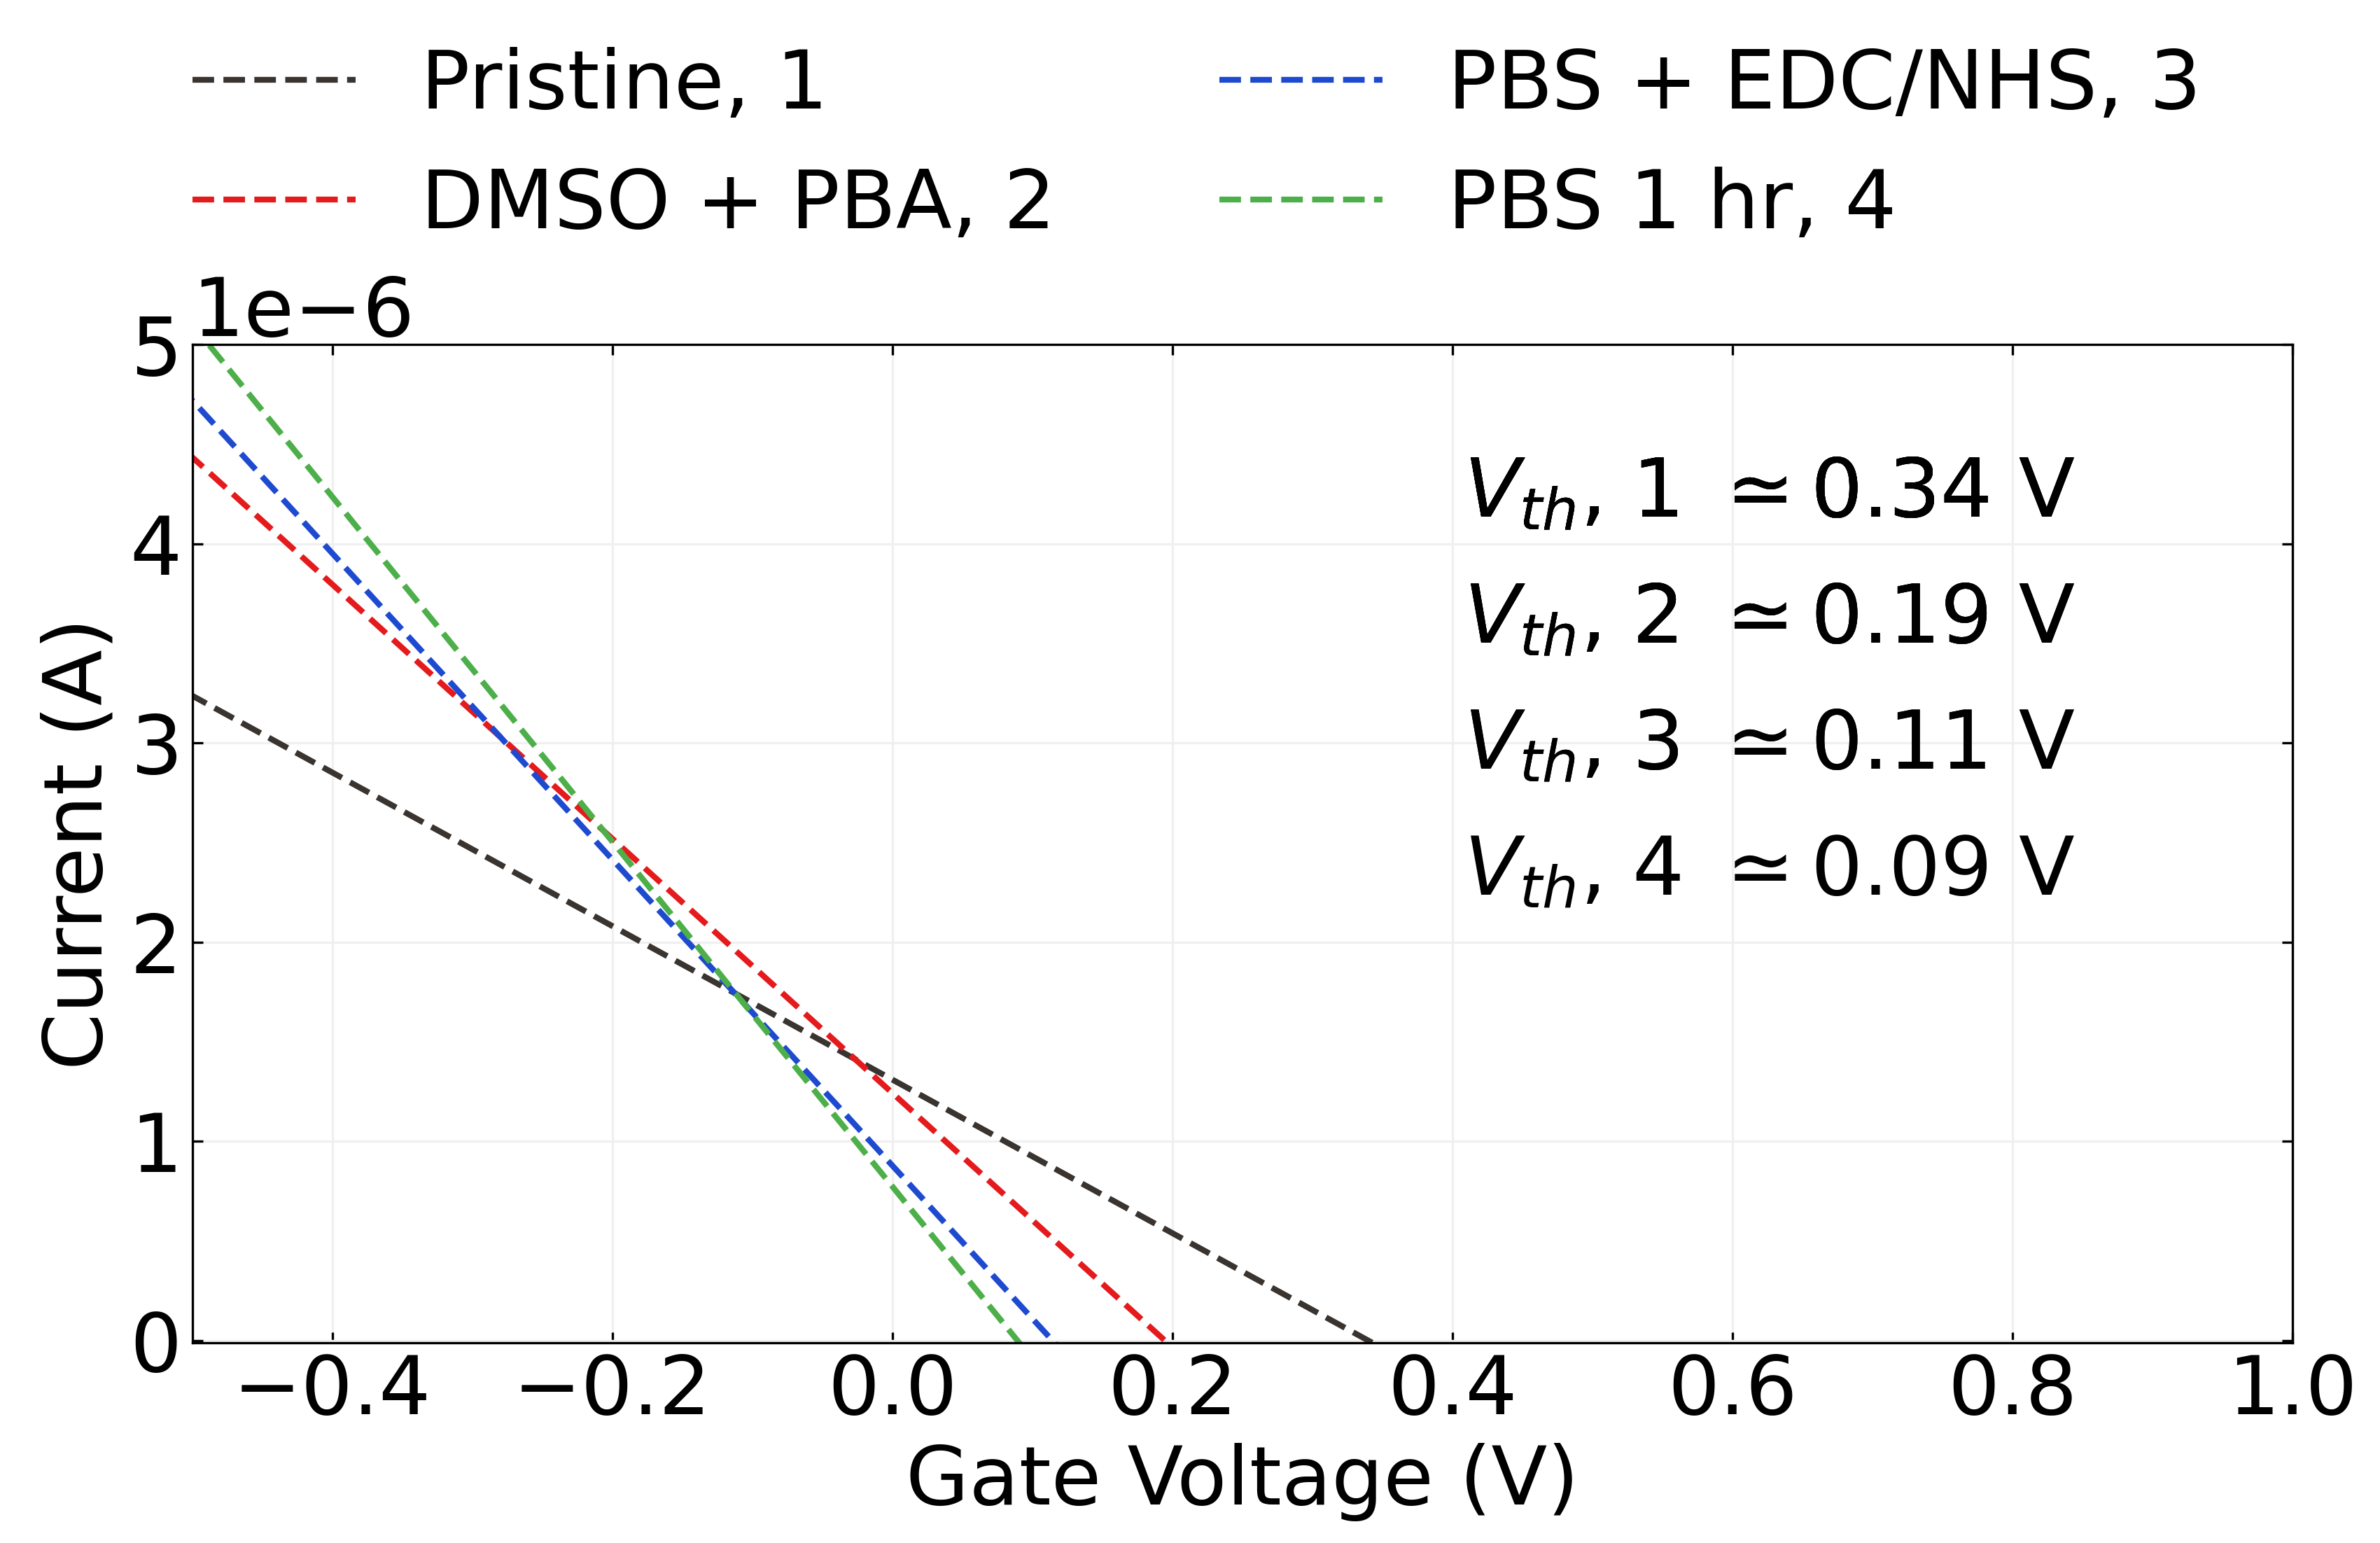
\includegraphics{figures/ch6/NTQ24C10_ch3_comparison_4.png}

}

}

\end{minipage}%
%
\begin{minipage}[t]{0.01\linewidth}

{\centering 

~

}

\end{minipage}%

\caption[Transfer characteristics of a carbon nanotube transistor,
before and after functionalisation with PBA or PBA/EDC/NHS, as well as
after submersion in fresh PBS, alongside linear fits to the subthreshold
slope of each curve in the forward
direction.]{\label{fig-pba-functionalisation-threshold-shift}Transfer
characteristics of a carbon nanotube transistor before functionalisation
alongside the transfer characteristics (a) after being submerged in DMSO
with 5 mM PBA in red, (b) after being submerged in PBS with 20 mM EDC
and 40 mM NHS in blue, and (c) after being submerged in fresh PBS in
green. The dashed lines in (d) are linear fits to the subthreshold slope
of each curve in the forward direction, and are shown alongside the
threshold voltages corresponding to each fit.}

\end{figure}

Subsequently, the device was rinsed with \(1 \times\) PBS and exposed to
20 mM EDC and 40 mM NHS in \(1 \times\) PBS electrolyte for 30 minutes.
Figure~\ref{fig-pba-functionalisation-threshold-shift} (b) shows the
change resulting from subsequent EDC/NHS exposure. When EDC/NHS is
added, a threshold shift of \(\Delta V \sim -0.08\) V was observed on
multiple channels. The exposure to EDC/NHS negatively shifts the
transfer characteristic curve, most likely due to the PBA present
reacting to form positively-charged \emph{O}-acylisourea esters and
negatively gating the attached carbon nanotube network {[}@Heller2008;
@Hermanson2013-4{]}.
Figure~\ref{fig-pba-functionalisation-threshold-shift} (c) shows that
this shift is not significantly affected by further exposure of the
channel to PBS. The lack of a change in gating may imply that hydrolysis
over the course of one hour is insufficient to hydrolyse a significant
proportion of the attached \emph{O}-acylisourea or PBASE back to PBA,
leaving them available for reaction with biomolecule amine groups. A
further test could be performed to see if leaving the device submerged
in water over a longer time period to check if ester hydrolysis
eventually affects threshold voltage in a significant manner, but this
was considered to be outside the scope of this work.

\hypertarget{attachment-of-peglyated-pyrene-based-linkers}{%
\subsection{Attachment of PEGlyated Pyrene-Based
Linkers}\label{attachment-of-peglyated-pyrene-based-linkers}}

\hypertarget{sec-NTA-biotin-PEG}{%
\subsubsection{Pyrene-NTA, Pyrene-Biotin and
PEGylation}\label{sec-NTA-biotin-PEG}}

Through chemical coupling/conjugation, it is possible to replace the NHS
ester group on PBASE with other groups that can undergo binding
reactions with proteins. Unlike PBASE, these groups do not suffer the
drawback of being readily hydrolysed. For example, PBASE can be modified
with N\(\alpha\),N\(\alpha\)-Bis(carboxymethyl)-L-lysine hydrate (also
known as N-(5-Amino-1-carboxypentyl)iminodiacetic acid, amine-NTA,
AB-NTA) to produce pyrene-nitrilotriacetic acid. The attached NTA group
is able to chelate with metal ions such as Cu\(^{2+}\) or Ni\(^{2+}\),
which then can then coordinate with polyhistidine-tags attached to a
protein {[}@Holzinger2011; @Fruh2011; @Amano2016; @Chang2017{]}. Use of
Cu\(^{2+}\) ions over Ni\(^{2+}\) gives stronger histidine bonding and
less non-specific adsorption {[}@Chang2017{]}. Functionalisation using
the NTA-Ni\(^{2+}\) chemistry was successfully used to attach mammalian
odorant receptors to a single carbon nanotube for detection of eugenol
vapour in real-time {[}@Goldsmith2011{]}. Pyrene-biotin (pyrene butanol
biotin ester) can also be produced for attaching avidin or strepavidin
{[}@Holzinger2011{]}. As avidin and strepavidin are tetrameric, they can
be attached to both pyrene-biotin and biotinylated avi-tagged proteins
simultaneously via strong non-covalent bonding, therefore linking the
transducer and receptor {[}@Star2003a; @Dundas2013; @Hermanson2013-11;
@Fairhead2015{]}. As the presence of his-tags and avi-tags on proteins
can be readily controlled, these methods offer improved specificity and
directionality over the traditional amide bonding seen earlier.

It is also possible to attach biocompatible {[}@Chen2004{]} polyethylene
glycol (PEG) chains to a pyrene group and modify them with reactive
groups such as NTA and biotin to attach proteins in the manner outlined
in the previous paragraph {[}@Hermanson2013-18; @Meran2018{]}. Once
modified with PEG, the hydrophilicity of the PEG increases the water
solubility of pyrene linkers, making it possible to perform a full
functionalisation procedure exclusively in aqueous solution
{[}@Chen2004; @Hermanson2013-18{]}. By setting the length of the PEG
chain, the size of the linker molecule can be controlled; selection of a
short chain is important to ensure attached receptors remain within the
Debye length of the transducer {[}@Shkodra2021{]}. Note that PEG
naturally repels proteins and can also bond to carbon nanotubes, and
both behaviours have uncertain implications for successful protein
functionalisation {[}@Chen2004{]}. However, functionalisation of both
carbon nanotube and graphene transducers with pyrene-PEG-biotin (PPB)
has previously been used for the successful detection of streptavidin
{[}@Star2003a; @Miki2019{]}. PEG is also charge neutral, so its presence
is not expected to significantly affect device characteristics
{[}@Chen2004{]}.

The PEGlyated linkers used in the following sections were purchased
pre-prepared. Pyrene-PEG-NTA (2 kDa) was purchased from Nanocs, while
pyrene-PEG-FITC (2 kDa, 10 kDa), pyrene-PEG-rhodamine (3.4 kDa),
mPEG-Pyrene (10 kDa) and pyrene-PEG-biotin (10 kDa) were purchased from
Creative PEGworks.

\hypertarget{sec-impediments}{%
\subsection{Identifying Functionalisation Obstacles using Fluorescence
Microscopy}\label{sec-impediments}}

\hypertarget{sec-fluorescence-remarks}{%
\subsubsection{General Overview}\label{sec-fluorescence-remarks}}

Various dyes and fluorescent tags were used to investigate approaches
for identifying successful attachment of biomolecules to a carbon
nanotube or graphene surface with fluorescence microscopy. The dyes
included fluorescein isothiocyanate (FITC), Rhodamine B and Cyanine 3
(Cy3). Green fluorescent protein was also used for this testing process.
It is important to note that these dyes and the GFP chromophore all
contain benzene rings which are able to pi-stack with carbon rings to
some degree {[}@Nakayama-Ratchford2007; @Tang2012; @Khrenova2019;
@Qiu2019{]}. However, there is also significant variation in the extent
to which this pi-stacking occurs, which can be seen by comparing
Figure~\ref{fig-FITC-rhodamine-B} (a) and
Figure~\ref{fig-FITC-rhodamine-B} (b). Here, a clear, specific
interaction is seen between Rhodamine B and graphene, but little
interaction between FITC and graphene is observed, even when a longer
exposure time is used when imaging. Whether the addition of pyrene
linker groups to these dyes or dye-modified biomolecules was able to
improve attachment was next investigated. This process led to the
identification of multiple issues that could impede a successful device
functionalisation.

\begin{figure}

\begin{minipage}[t]{0.03\linewidth}

{\centering 

\raisebox{-\height}{


\includegraphics{figures/(a).png}

}

}

\end{minipage}%
%
\begin{minipage}[t]{0.01\linewidth}

{\centering 

~

}

\end{minipage}%
%
\begin{minipage}[t]{0.45\linewidth}

{\centering 

\raisebox{-\height}{

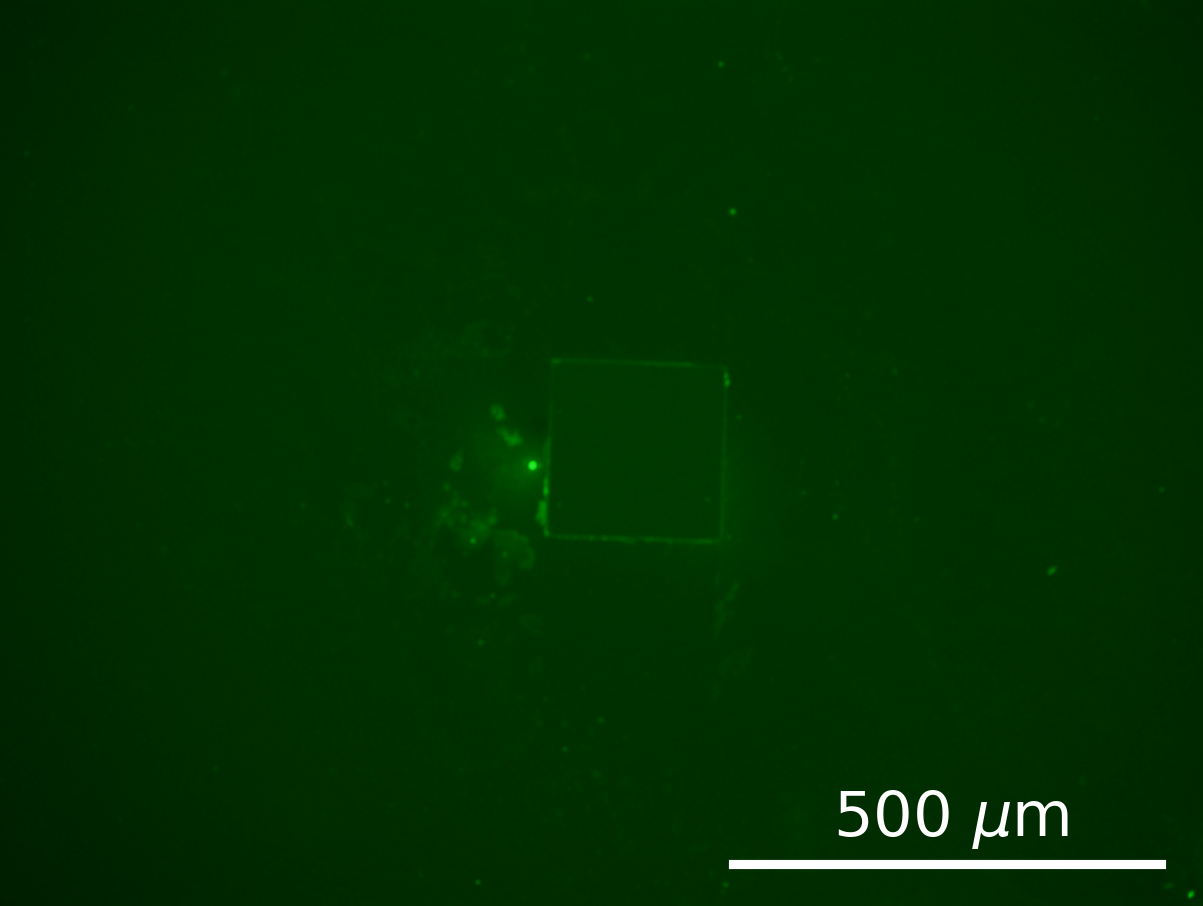
\includegraphics{figures/ch6/NGW8D1_FITC_6.5sexposure_10X_221121.png}

}

}

\end{minipage}%
%
\begin{minipage}[t]{0.01\linewidth}

{\centering 

~

}

\end{minipage}%
%
\begin{minipage}[t]{0.03\linewidth}

{\centering 

\raisebox{-\height}{


\includegraphics{figures/(b).png}

}

}

\end{minipage}%
%
\begin{minipage}[t]{0.01\linewidth}

{\centering 

~

}

\end{minipage}%
%
\begin{minipage}[t]{0.45\linewidth}

{\centering 

\raisebox{-\height}{

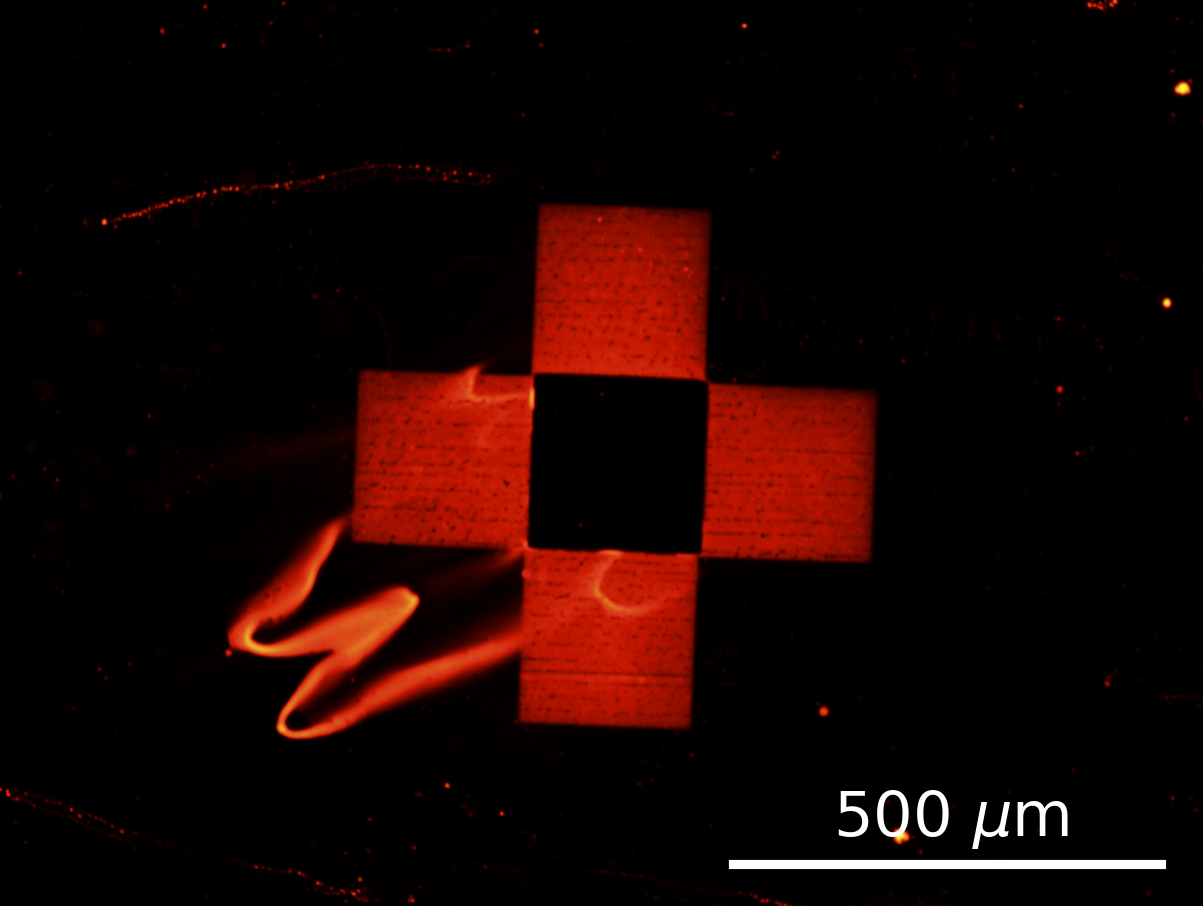
\includegraphics{figures/ch6/NGW8D4_rhodamineB_cornergraphene_221110.png}

}

}

\end{minipage}%
%
\begin{minipage}[t]{0.01\linewidth}

{\centering 

~

}

\end{minipage}%

\caption[Four 200 µm \(\times\) 200 µm graphene squares modified with
the dyes fluorescein isothiocyanate (FITC) and Rhodamine
B.]{\label{fig-FITC-rhodamine-B}Four 200 µm \(\times\) 200 µm graphene
squares modified with the dyes (a) fluorescein isothiocyanate (FITC) and
(b) Rhodamine B. No pyrene/PEG/pyrene-PEG was attached to these dyes. In
(a), an FITC filter and 6.5 s exposure time was used, and in (b) a Texas
Red filter and 1.4 s exposure time was used.}

\end{figure}

Both SU8 and AZ\(^\circledR\) 1518 photoresist fluoresced under a
variety of microscope filters, resulting from light interacting with the
photoactive component present in both resists {[}@Pai2007{]}. This
background fluorescence was found to drown out fluorescence from a
dye-functionalised device channel, and so photoresist encapsulated
devices were not used for fluorescence imaging. (Consider a photograph
of a dim outdoor lamp; if the photograph was taken on a starless night,
the light from the lamp would show up clearly, but with the sun out the
light would be very difficult to see regardless of how the photograph
was taken). A different type of encapsulation could potentially be used
to verify linker attachment with fluorescence after a device has been
encapsulated. These alternative encapsulation methods for use with
fluorescence microscopy are discussed in
\textbf{?@sec-future-work-fabrication}.

\hypertarget{sec-photoresist-contamination}{%
\subsubsection{Photoresist
Contamination}\label{sec-photoresist-contamination}}

An functionalisation issue quickly encountered when characterising
pyrene-PEG-FITC (PPF) functionalisation via fluorescence microscopy was
an unwanted secondary interaction between the linker and residual
photoresist. Figure~\ref{fig-photoresist-contamination} (a) and
Figure~\ref{fig-photoresist-contamination} (b) are fluorescence images
of SU8 encapsulation (using the pre-2023 mask) before and after being
exposed to PPF. Despite the same microscope settings being used to take
the images (filter, ISO, contrast, exposure time), the SU8 exposed to
PPF appears much brighter than the pristine SU8. This result indicates
that the linker appears to have an extensive interaction with the
photoresist via an unknown mechanism. No fluorescence is seen from the
device channel. The length of exposure time required to see fluorescence
from the modified channel would lead to fluorescence from the modified
linker attached to the photoresist (as well as the photoresist itself)
flooding the image with light. Therefore, it is not clear whether the
carbon nanotubes have been functionalised with the dye-modified linker.
Out of caution, we can assume that this secondary interaction is not
desirable for successful functionalisation.

\begin{figure}

\begin{minipage}[t]{0.03\linewidth}

{\centering 

\raisebox{-\height}{


\includegraphics{figures/(a).png}

}

}

\end{minipage}%
%
\begin{minipage}[t]{0.01\linewidth}

{\centering 

~

}

\end{minipage}%
%
\begin{minipage}[t]{0.45\linewidth}

{\centering 

\raisebox{-\height}{

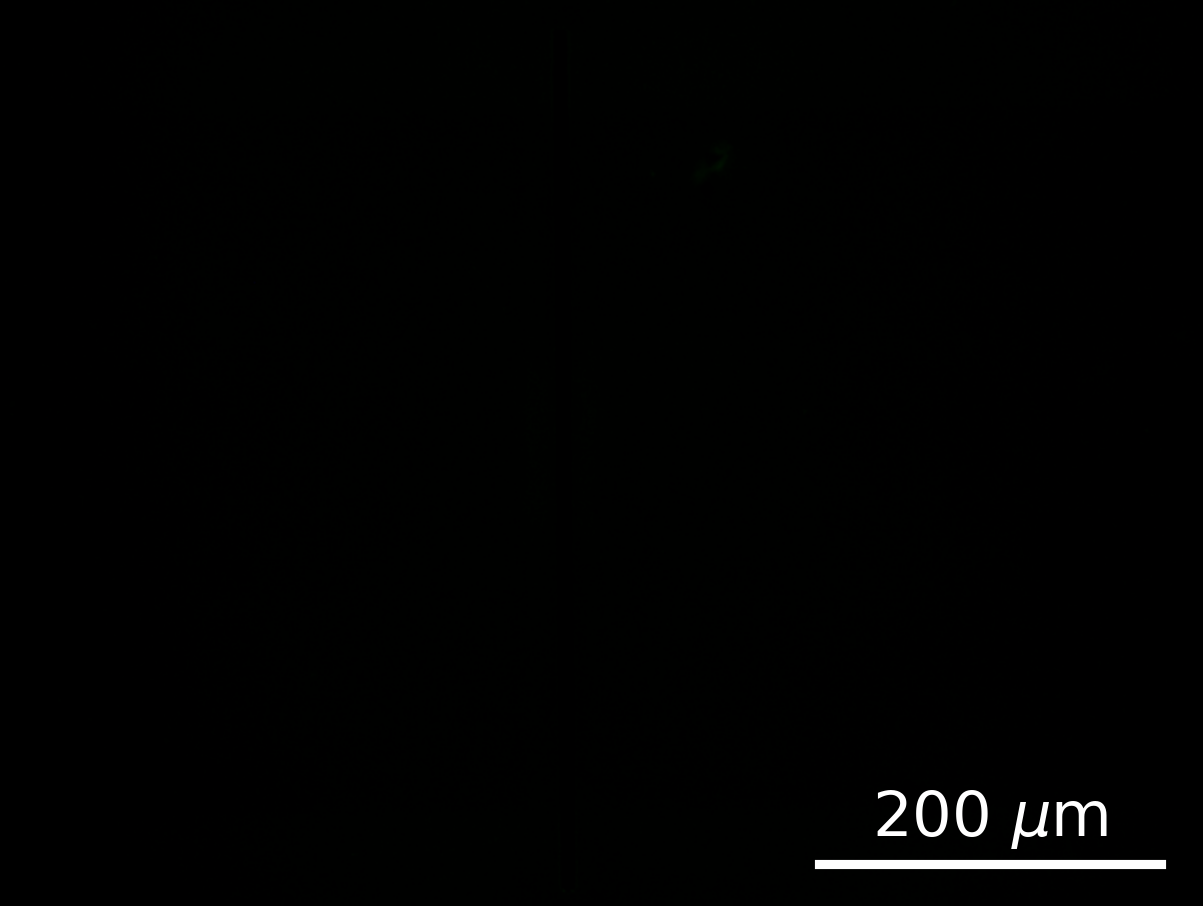
\includegraphics{figures/ch6/modified_SU8only_FITCfilter_channel2_350ms_12.6X_221207.png}

}

}

\end{minipage}%
%
\begin{minipage}[t]{0.01\linewidth}

{\centering 

~

}

\end{minipage}%
%
\begin{minipage}[t]{0.03\linewidth}

{\centering 

\raisebox{-\height}{


\includegraphics{figures/(b).png}

}

}

\end{minipage}%
%
\begin{minipage}[t]{0.01\linewidth}

{\centering 

~

}

\end{minipage}%
%
\begin{minipage}[t]{0.45\linewidth}

{\centering 

\raisebox{-\height}{

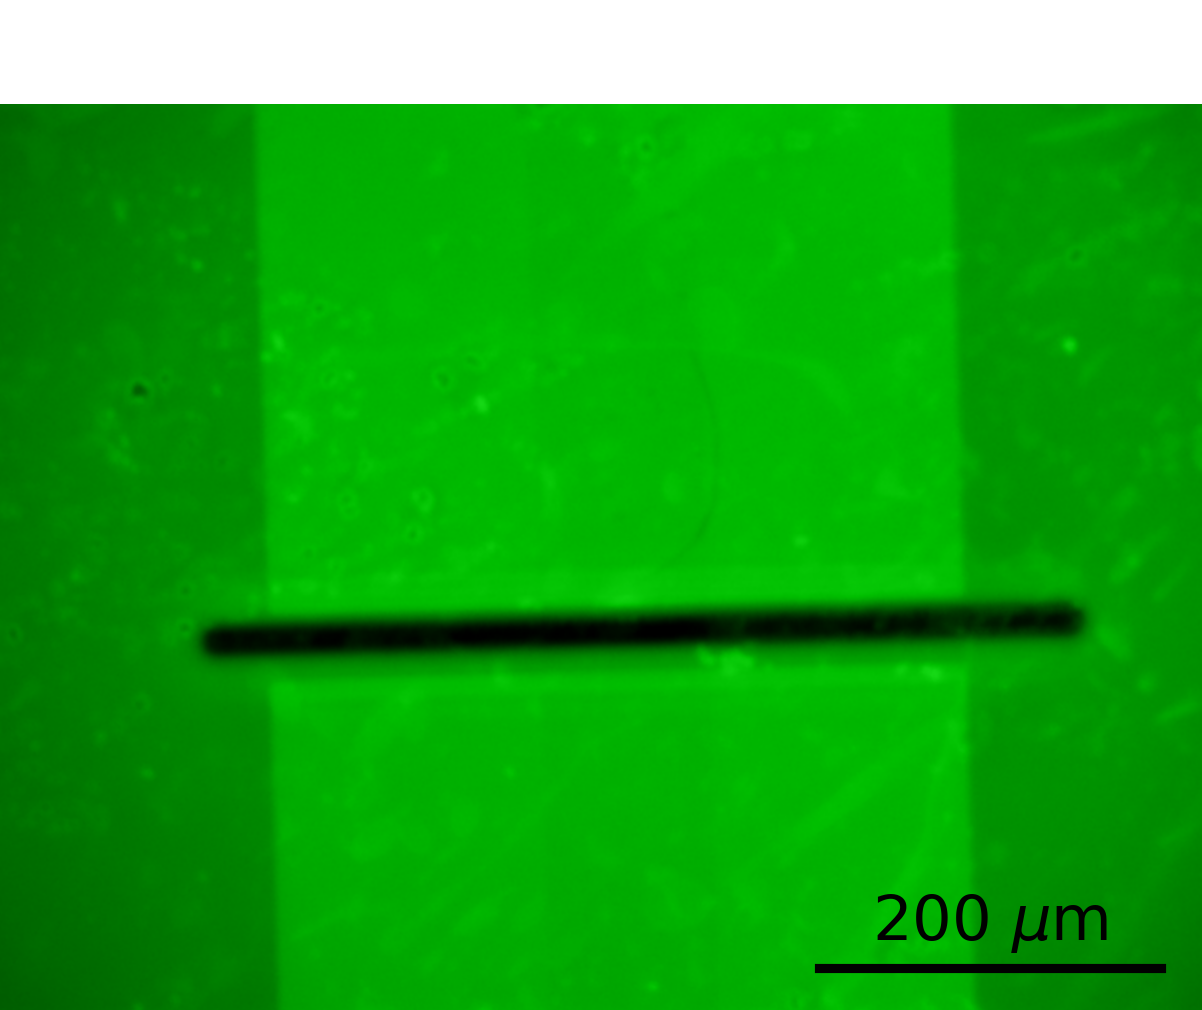
\includegraphics{figures/ch6/modified_CNT20_1mMPPF_channel8_350ms_12.6X_221124.png}

}

}

\end{minipage}%
%
\begin{minipage}[t]{0.01\linewidth}

{\centering 

~

}

\end{minipage}%
\newline
\begin{minipage}[t]{0.03\linewidth}

{\centering 

\raisebox{-\height}{


\includegraphics{figures/(c).png}

}

}

\end{minipage}%
%
\begin{minipage}[t]{0.01\linewidth}

{\centering 

~

}

\end{minipage}%
%
\begin{minipage}[t]{0.45\linewidth}

{\centering 

\raisebox{-\height}{

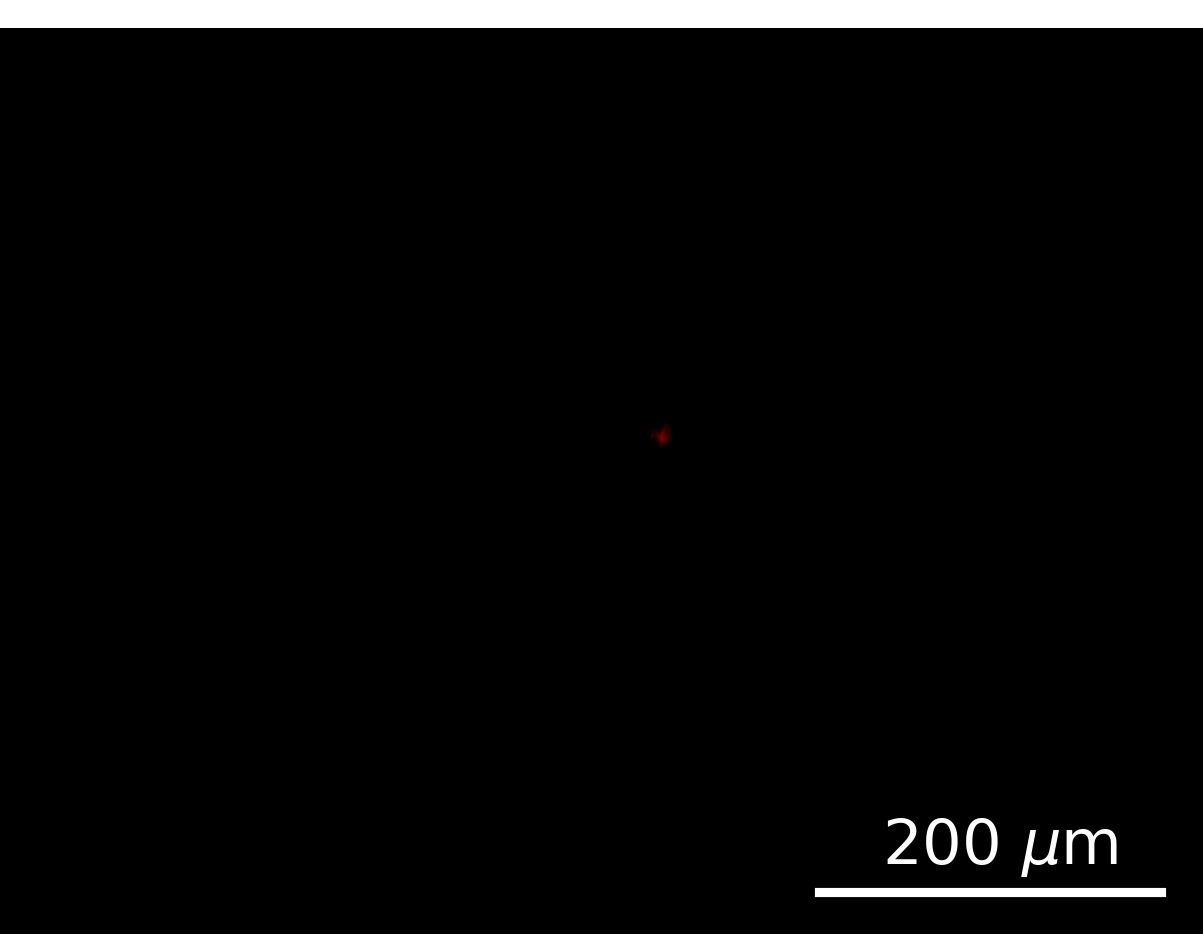
\includegraphics{figures/ch6/modified_Ccontrol_ch2_mCherry_10sexposure_highcontrast_12.6X.png}

}

}

\end{minipage}%
%
\begin{minipage}[t]{0.01\linewidth}

{\centering 

~

}

\end{minipage}%
%
\begin{minipage}[t]{0.03\linewidth}

{\centering 

\raisebox{-\height}{


\includegraphics{figures/(d).png}

}

}

\end{minipage}%
%
\begin{minipage}[t]{0.01\linewidth}

{\centering 

~

}

\end{minipage}%
%
\begin{minipage}[t]{0.45\linewidth}

{\centering 

\raisebox{-\height}{

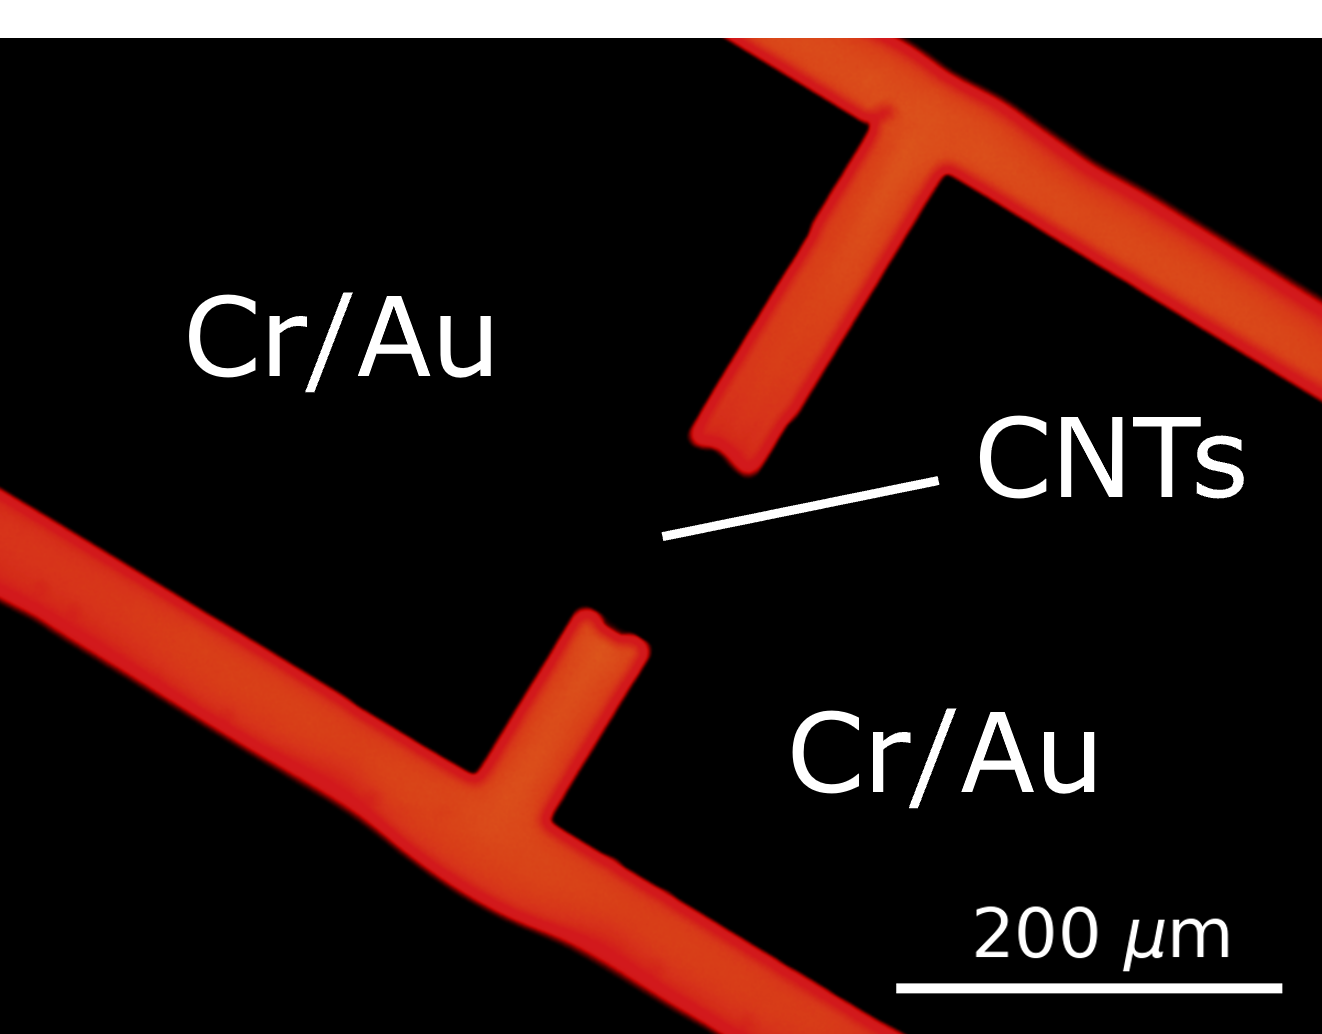
\includegraphics{figures/ch6/modified_C1_ch5_mCherry_10sexposure_highcontrast_12.6X.png}

}

}

\end{minipage}%
%
\begin{minipage}[t]{0.01\linewidth}

{\centering 

~

}

\end{minipage}%
\newline
\begin{minipage}[t]{0.03\linewidth}

{\centering 

\raisebox{-\height}{


\includegraphics{figures/(e).png}

}

}

\end{minipage}%
%
\begin{minipage}[t]{0.01\linewidth}

{\centering 

~

}

\end{minipage}%
%
\begin{minipage}[t]{0.45\linewidth}

{\centering 

\raisebox{-\height}{

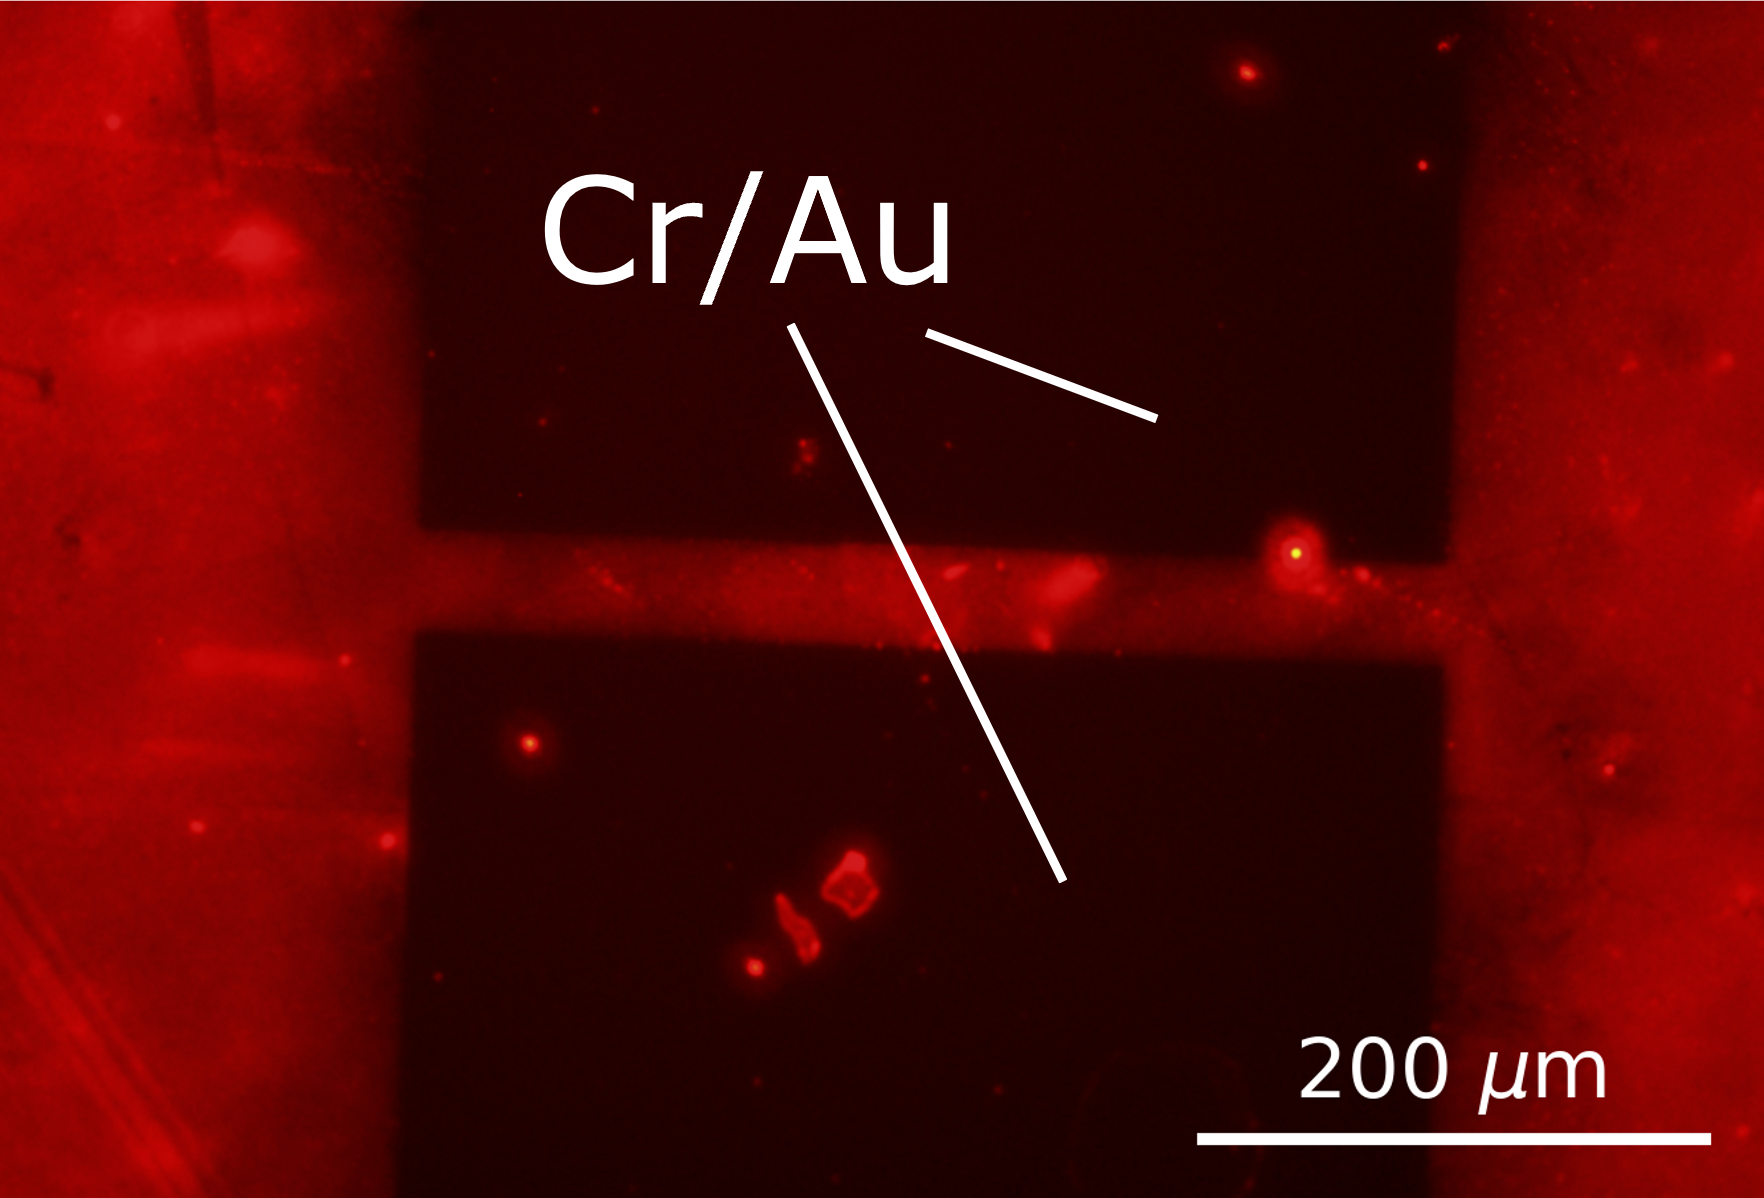
\includegraphics{figures/ch6/modified_softbake1minacetonerinse_aptamer_ch3_mCherry_30sexposure_highcontrast_ISO200_12.6X.png}

}

}

\end{minipage}%
%
\begin{minipage}[t]{0.01\linewidth}

{\centering 

~

}

\end{minipage}%
%
\begin{minipage}[t]{0.03\linewidth}

{\centering 

\raisebox{-\height}{


\includegraphics{figures/(f).png}

}

}

\end{minipage}%
%
\begin{minipage}[t]{0.01\linewidth}

{\centering 

~

}

\end{minipage}%
%
\begin{minipage}[t]{0.45\linewidth}

{\centering 

\raisebox{-\height}{

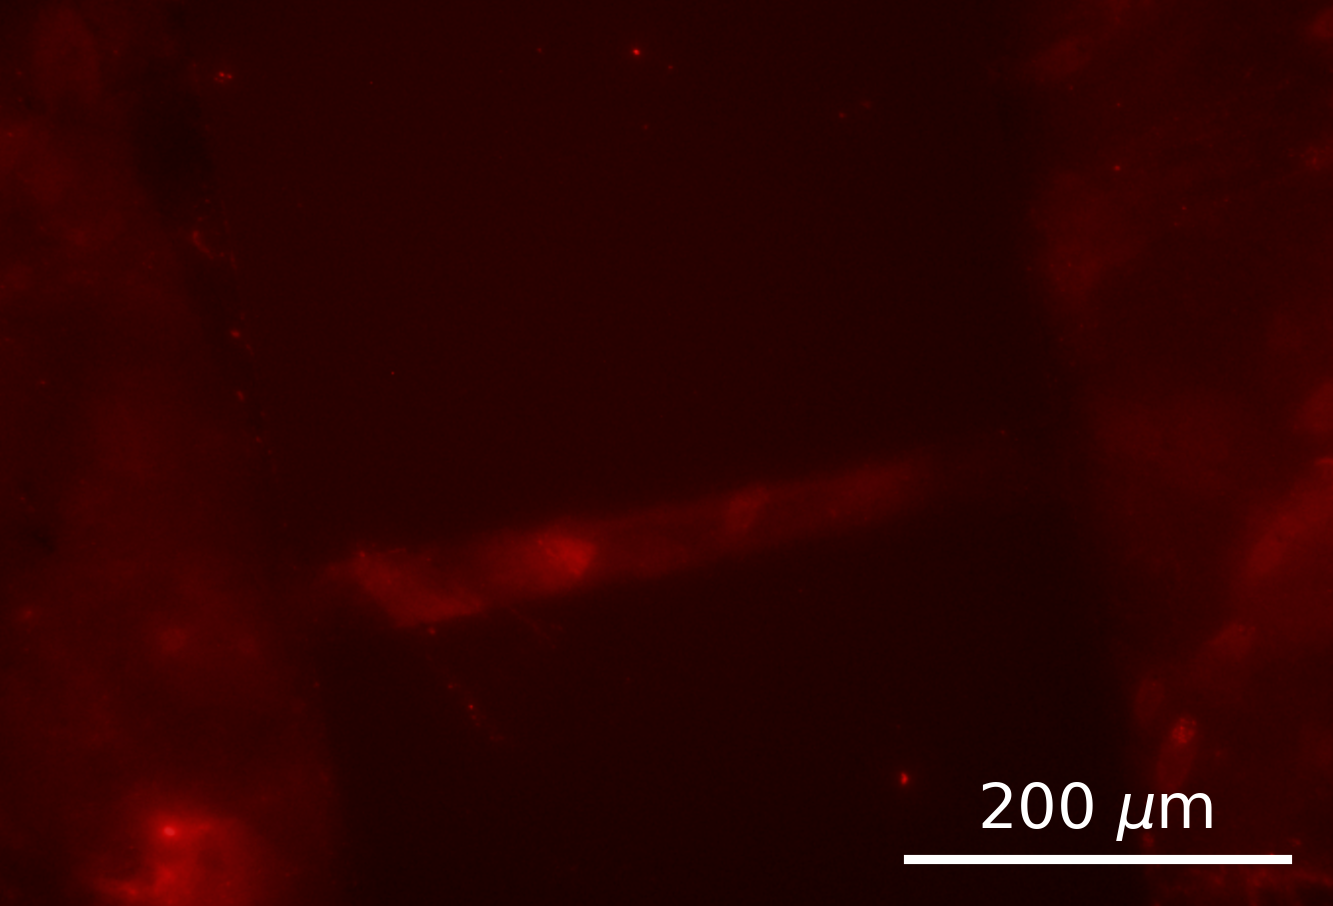
\includegraphics{figures/ch6/modified_hardbake_aptamer_ch3_mCherry_30sexposure_highcontrast_ISO200_12.6X.png}

}

}

\end{minipage}%
%
\begin{minipage}[t]{0.01\linewidth}

{\centering 

~

}

\end{minipage}%

\caption[Fluorescence images demonstrating the interaction of
fluorescent-tagged linker or aptamer with photoresist present on a
carbon nanotube network device
surface.]{\label{fig-photoresist-contamination}A fluorescence image of a
SU8-encapsulated carbon nanotube device is shown in (a), while (b) shows
the same channel after modification with an solution of 1 mM
Pyrene-PEG-FITC. A 0.35 s exposure time and FITC filter were used for
(a)-(b). The fluorescence image in (c) shows an unencapsulated channel,
while (d) shows the same channel after Cy3-tagged aptamer exposure. A 10
s exposure time and mCherry filter were used for (c)-(d). The
fluorescence images in (e) and (f) show devices pre-coated with a thin
layer of photoresist then submerged in Cy3-tagged aptamer, where the
device in (f) was hardbaked before aptamer exposure. An mCherry filter
and 30 s exposure time were used for for (e)-(f).}

\end{figure}

A similar interaction was seen between AZ\(^\circledR\) 1518 photoresist
and fluorescent-tagged, amine-terminated aptamer. An unencapsulated
carbon nanotube network device, fabricated using the pre-Jun 2022
process outlined in \textbf{?@sec-fabrication}, was incubated with 500
nM Cy3-tagged aptamer in Tris solution at 4 °C overnight. The aptamer
was first denatured by heating in a water bath at 95 °C for 5 minutes,
then cooling in an ice bath for 10 minutes before use.
Figure~\ref{fig-photoresist-contamination} (c) and
Figure~\ref{fig-photoresist-contamination} (d) are fluorescence images
of the device channel region before and after exposure to aptamer. A
thick red ring is visible around the electrodes after functionalisation,
despite no PBASE being used to tether the amine-terminated aptamer. It
appears that these bright patches correspond to residual photoresist
which has not been completely removed from the carbon nanotube square in
the development process. These patches have then interacted with the
aptamer, causing them to appear bright under the fluorescence
microscope. Beyond potentially interfering with functionalisation,
photoresist residue blocking a device channel will prevent interaction
with the Tris solution and prevent sensing.

To test whether residual resist could be prevented from interacting with
aptamer by crosslinking the resist, two unencapsulated devices were
prepared as follows. Devices were first spincoated with AZ\(^\circledR\)
1518 in the manner described in \textbf{?@sec-fabrication}. Next, the
majority of resist was removed by soaking the device in acetone for 1
minute. This process left a thin coating of photoresist on the devices.
One of these devices was then hardbaked at 200 °C for 1 hour. Both
devices were subsequently functionalised in the following manner:

\begin{enumerate}
\def\labelenumi{\arabic{enumi}.}
\item
  The unencapsulated device was submerged in 1 mM PBASE in methanol
  solution for 1 hour.
\item
  The device was then rinsed with methanol and Tris.
\item
  1 µM Cy3-tagged aptamer was denatured by heating in a water bath at
  95°C for 5 minutes, then cooling in an ice bath for 10 minutes before
  use.
\item
  The device was incubated with aptamer in Tris at 4 °C overnight.
\end{enumerate}

Fluorescence microscope images of channels from each device are shown in
Figure~\ref{fig-photoresist-contamination} (e) and
Figure~\ref{fig-photoresist-contamination} (f), where the latter is the
device hardbaked before functionalisation. By comparing the two images,
it is apparent that hardbaking the AZ\(^\circledR\) 1518 photoresist
significantly reduces the amount of fluorescent aptamer attached to the
surface. This result is an indication that sufficient heating of the
photoresist can prevent it interacting with PBASE or amine-tagged
biological material. However, there is still some Cy3-tagged aptamer
fluorescence visible in Figure~\ref{fig-photoresist-contamination} (f).
It appears that hardbaking has not completely prevented photoresist from
interacting with the aptamer. It is possible that heating from the
bottom of the device is insufficient to hardbake the photoresist layer
completely, an effect that would be amplified for the thick photoresist
layer on encapsulated devices. Therefore, from Jun 2023 onwards devices
were vacuum annealed for 1 hour at 150 °C prior to functionalisation.
This approach was taken to ensure photoresist was heated from above as
well as below and made chemically inert across its surface.

This result demonstrates the use of fluorescence microscopy as a tool to
detect residue and test suitable residue elimination measures. Further
testing showed that performing a 1 minute flood exposure (for positive
resist only) then placing a device in AZ\(^\circledR\) 326 developer for
three minutes (for both positive and negative resist) was highly
effective at removing photoresist residue. Both these development and
annealing techniques were used for all functionalised devices in
subsequent sections.

\hypertarget{sec-hydrophobicity}{%
\subsubsection{Hydrophobicity of Carbon Nanotubes and
Graphene}\label{sec-hydrophobicity}}

As PEGlyated linker dissolves well in aqueous solution, initial
fluorescence imaging focused on functionalising devices with these
linkers dissolved in \(1 \times\) PBS. It was hoped that by keeping the
device channels in a pH-controlled environment, the channel surface
would be made more suitable for the attached receptors.
Figure~\ref{fig-silicon-dioxide-interaction} (a) shows a graphene film
after exposure to pyrene-PEG-rhodamine (PPR) in \(1 \times\) PBS
solution for 1 hour. The pyrene-PEG-rhodamine has interacted with the
SiO\(_2\) substrate (discussed further in
Section~\ref{sec-pyrene-interactions}) but not the graphene film. The
graphene has not attached to the pyrene or rhodamine due to the highly
hydrophobic graphene surface repelling the surrounding solution,
preventing pi-stacking from occurring. The hydrophobicity of the
graphene surface is not intrinsic to graphene. Instead, it results from
a hydrocarbon layer which forms on the channel surface when exposed to
air, primarily composed of long-chain alkanes {[}@Ashraf2014;
@Palinkas2022{]}. A hydrophobic layer wiil also form on carbon nanotube
networks {[}@Stando2019; @Park2022{]}. Treatment with oxygen plasma at 5
W for 15 s has previously been found to remove this hydrocarbon layer,
restoring the intrinsic hydrophilicity of graphene {[}@Shin2010{]}.
Storing the graphene surface in deionised water rather than air prevents
the return of this hydrocarbon layer {[}@Ashraf2014{]}. The use of a
relatively low power plasma ensures damage to the graphene layer is
minimised.

Treatment of an unencapsulated carbon nanotube network device at 5 W for
15 s at 300 mTorr greatly reduced the contact angle of a water droplet
placed on the device surface. The water droplet before and after plasma
treatment is shown inset in Figure~\ref{fig-silicon-dioxide-interaction}
(a) and Figure~\ref{fig-silicon-dioxide-interaction} (b) respectively. A
graphene film was then functionalised with pyrene-PEG-rhodamine in
\(1 \times\) PBS in the same manner as for the film in
Figure~\ref{fig-silicon-dioxide-interaction} (a), except with the same
plasma treatment performed on the film less than 1 minute before
functionalisation. The result is shown in
Figure~\ref{fig-silicon-dioxide-interaction} (b). The graphene now
appears to interact with the pyrene-PEG-rhodamine. These results both
indicate that the plasma treatment is increasing the hydrophilicity of
the device surface, improving the ability of pyrene-PEG-rhodamine to
\(\pi\)-stack with graphene. The disadvantage of this procedure is that
the plasma cleaning introduces defects to the graphene surface which may
be undesirable for device electrical behaviour. Furthermore, it was
often found that devices functionalised in this manner had their
conductance drop significantly after functionalisation, even though
plasma treatment itself did not significantly alter device conductance.
Solvent was therefore used for the initial linker functionalisation in
\textbf{?@sec-biosensing-iORs}, as a plasma cleaning step was not
required for linker attachment.

\hypertarget{sec-pyrene-interactions}{%
\subsubsection{Substrate Interaction with Linker
Molecules}\label{sec-pyrene-interactions}}

Another issue that arose when verifying surface functionalisation was
the interaction between pyrene linker and the SiO\(_2\) substrate. This
interaction meant it was difficult to discern whether the pyrene group
was interacting in a specific manner with the channel film. It was
confirmed that pyrene-PEG was interacting with SiO\(_2\), rather than
residual photoresist or nanomaterial, by performing a
pyrene-PEG-rhodamine functionalisation on pristine SiO\(_2\), as shown
in Figure~\ref{fig-silicon-dioxide-interaction} (c). The PEGlyated
linker supplier suggested that the surface should be thoroughly rinsed
with surfactant to remove weakly-bound pyrene-PEG-FITC attached to the
SiO\(_2\), while preserving the pyrene-PEG-FITC strongly attached via
pi-stacking to the graphene or carbon nanotube film
{[}@CreativePEGworks2022{]}. A novel process was then developed to
remove pyrene-PEG-FITC from the SiO\(_2\). The film was rinsed with DI
water for 30 s, placed in m-CNT dispersion solution (NanoIntegris) for 5
minutes at 70 °C while agitating with a pipette, and finally rinsed with
DI water, ethanol, acetone, IPA and nitrogen dried. A the graphene
region before cleaning is shown in
Figure~\ref{fig-silicon-dioxide-interaction} (d), while the results of
cleaning are shown in Figure~\ref{fig-silicon-dioxide-interaction} (e)
and Figure~\ref{fig-silicon-dioxide-interaction} (f). The majority of
pyrene-PEG-FITC was removed in regions with no graphene, but remained
where graphene was present, indicating specific, pi-stacking interaction
took place between the pyrene-PEG-FITC and graphene. However, this
surfactant rinse step was not used when performing functionalisation
with biological materials, to prevent damage to the lipid membranes
used.

\begin{figure}

\begin{minipage}[t]{0.03\linewidth}

{\centering 

\raisebox{-\height}{


\includegraphics{figures/(a).png}

}

}

\end{minipage}%
%
\begin{minipage}[t]{0.01\linewidth}

{\centering 

~

}

\end{minipage}%
%
\begin{minipage}[t]{0.45\linewidth}

{\centering 

\raisebox{-\height}{

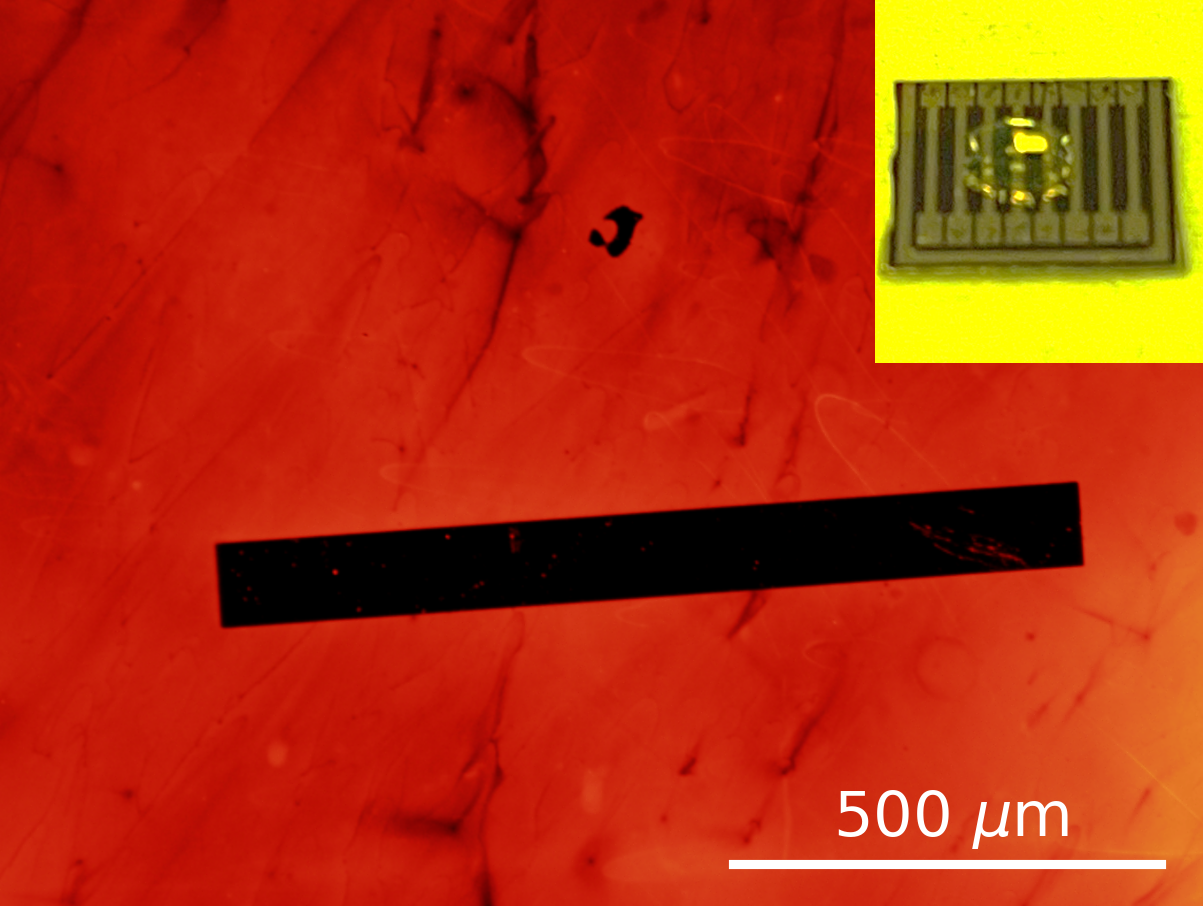
\includegraphics{figures/ch6/modified_NGW8D9_edgechannel_post10min50Cacetonerinse_221109.png}

}

}

\end{minipage}%
%
\begin{minipage}[t]{0.01\linewidth}

{\centering 

~

}

\end{minipage}%
%
\begin{minipage}[t]{0.03\linewidth}

{\centering 

\raisebox{-\height}{


\includegraphics{figures/(b).png}

}

}

\end{minipage}%
%
\begin{minipage}[t]{0.01\linewidth}

{\centering 

~

}

\end{minipage}%
%
\begin{minipage}[t]{0.45\linewidth}

{\centering 

\raisebox{-\height}{

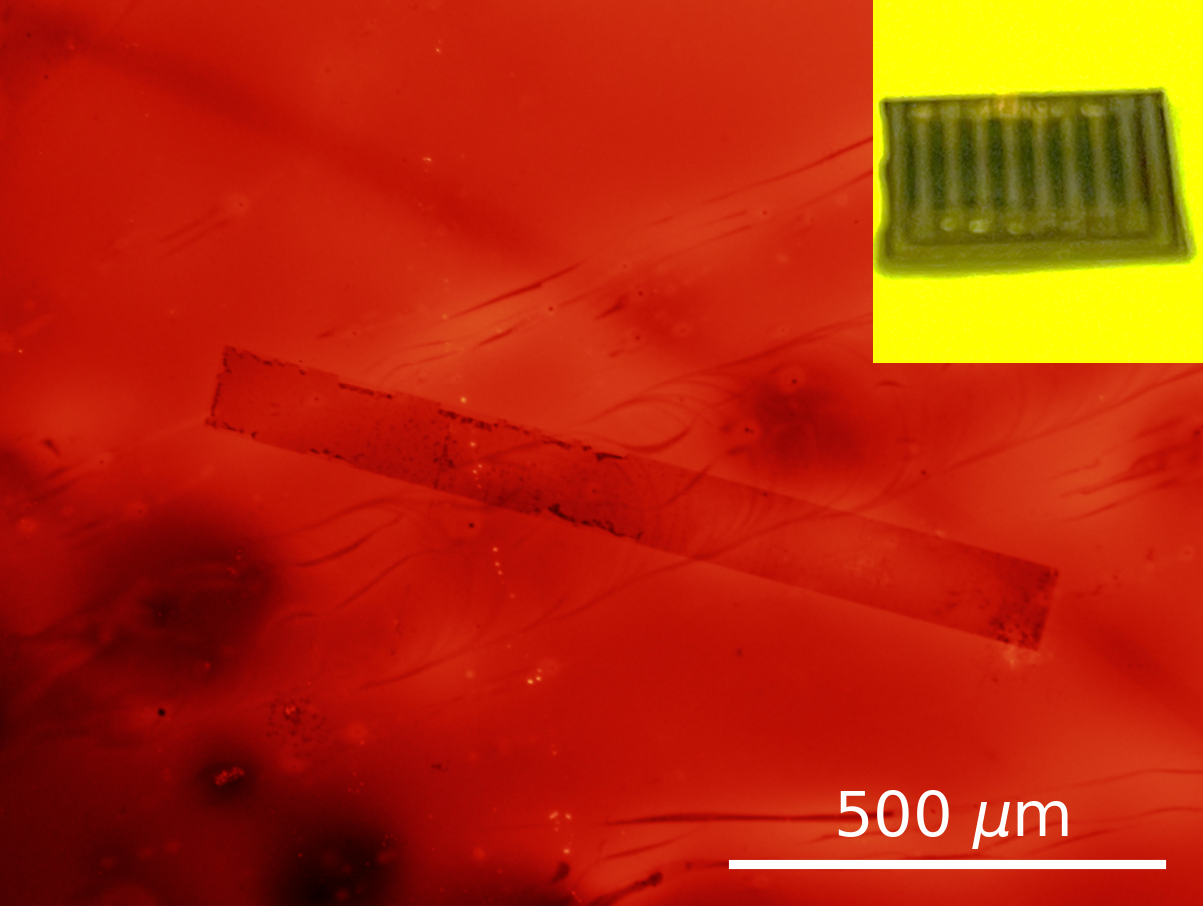
\includegraphics{figures/ch6/modified_NGW8D7_edgechannel_lowerexposuretime_221108.png}

}

}

\end{minipage}%
%
\begin{minipage}[t]{0.01\linewidth}

{\centering 

~

}

\end{minipage}%
\newline
\begin{minipage}[t]{0.03\linewidth}

{\centering 

\raisebox{-\height}{


\includegraphics{figures/(c).png}

}

}

\end{minipage}%
%
\begin{minipage}[t]{0.01\linewidth}

{\centering 

~

}

\end{minipage}%
%
\begin{minipage}[t]{0.45\linewidth}

{\centering 

\raisebox{-\height}{

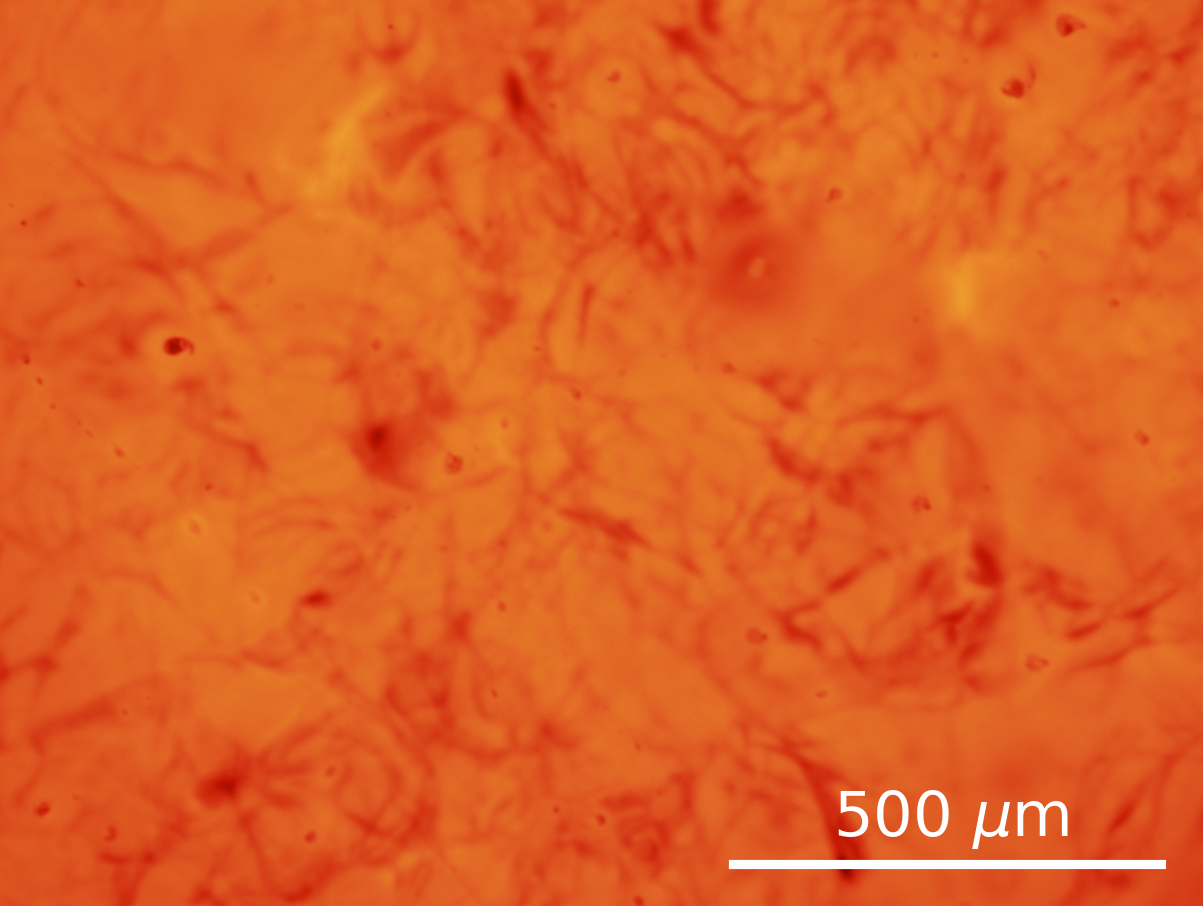
\includegraphics{figures/ch6/modified_SiO2_1mMPPR_2_221109.png}

}

}

\end{minipage}%
%
\begin{minipage}[t]{0.01\linewidth}

{\centering 

~

}

\end{minipage}%
%
\begin{minipage}[t]{0.03\linewidth}

{\centering 

\raisebox{-\height}{


\includegraphics{figures/(d).png}

}

}

\end{minipage}%
%
\begin{minipage}[t]{0.01\linewidth}

{\centering 

~

}

\end{minipage}%
%
\begin{minipage}[t]{0.45\linewidth}

{\centering 

\raisebox{-\height}{

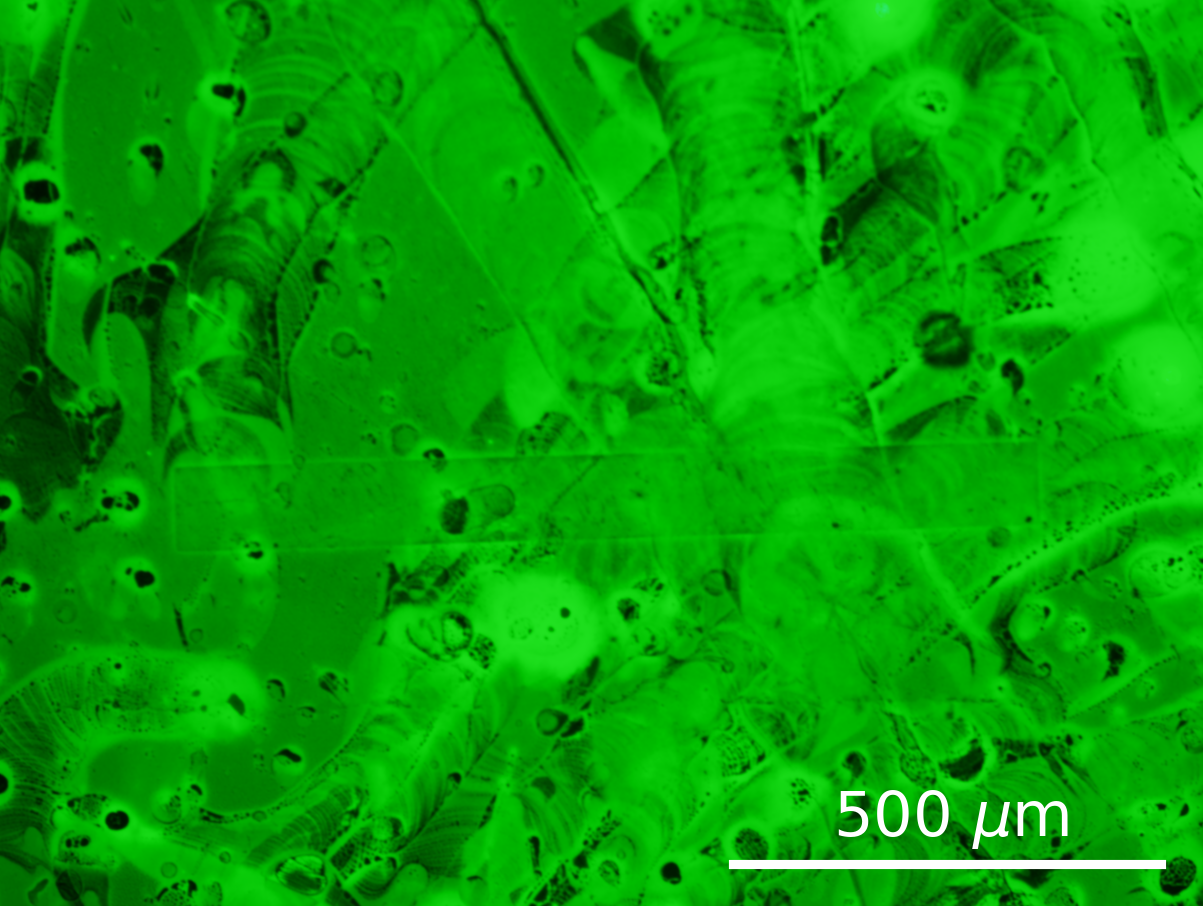
\includegraphics{figures/ch6/modified_NGW6D4_PyPEGFITC_channel2_1.6sexposure_10X_221122.png}

}

}

\end{minipage}%
%
\begin{minipage}[t]{0.01\linewidth}

{\centering 

~

}

\end{minipage}%
\newline
\begin{minipage}[t]{0.03\linewidth}

{\centering 

\raisebox{-\height}{


\includegraphics{figures/(e).png}

}

}

\end{minipage}%
%
\begin{minipage}[t]{0.01\linewidth}

{\centering 

~

}

\end{minipage}%
%
\begin{minipage}[t]{0.45\linewidth}

{\centering 

\raisebox{-\height}{

\includegraphics{figures/ch6/modified_NGW6D7_PyPEGFITC_channel3top_postmsurfclean_7.5sexposure_20X_221123.png}

}

}

\end{minipage}%
%
\begin{minipage}[t]{0.01\linewidth}

{\centering 

~

}

\end{minipage}%
%
\begin{minipage}[t]{0.03\linewidth}

{\centering 

\raisebox{-\height}{

\includegraphics{figures/(f).png}

}

}

\end{minipage}%
%
\begin{minipage}[t]{0.01\linewidth}

{\centering 

~

}

\end{minipage}%
%
\begin{minipage}[t]{0.45\linewidth}

{\centering 

\raisebox{-\height}{

\includegraphics{figures/ch6/modified_NGW6D7_PyPEGFITC_channel1_postmsurfclean_7.75sexposure_40X_221123.png}

}

}

\end{minipage}%
%
\begin{minipage}[t]{0.01\linewidth}

{\centering 

~

}

\end{minipage}%

\caption[Fluorescence images of a 1000 µm \(\times\) 100 µm graphene
channel, showing the effects of oxygen plasma cleaning and surfactant
rinsing on fluorescent linker
functionalisation.]{\label{fig-silicon-dioxide-interaction}Fluorescence
images of a 1000 µm \(\times\) 100 µm graphene channel. (a) was not
oxygen plasma cleaned before functionalisation with pyrene-PEG-rhodamine
(PPR), while (b) was oxygen plasma cleaned immediately before PPR
functionalisation. Insets show a water droplet on an unencapsulated
device before (a) and after (b) being treated with O\(_2\) plasma; (c)
shows a pristine SiO\(_2\) surface after PPR exposure. (a), (b) and (c)
were taken using a Texas Red filter and a 1.8 s exposure time. (d) was
functionalised with 1 mM PPF in PBS after oxygen plasma treatment, while
(e) and (f) were functionalised with 1 mM PPF after oxygen plasma
treatment, then cleaned with surfactant (m-CNT surfactant,
NanoIntegris). (d), (e) and (f) were taken using an FITC filter, with
1.6 s, 7.5 s and 7.75 s exposure times respectively.}

\end{figure}

\hypertarget{sec-coffee-ring}{%
\subsubsection{Coffee-Ring Effect}\label{sec-coffee-ring}}

From \textbf{?@tbl-pbase-functionalisation}, full device submersion
appears to be the most common approach for functionalisation with
solution containing linker molecules like PBASE. However, some groups
placed small droplets of solution onto the device channels when
functionalisation, and this approach was tested as part of the
fluorescence verification work. For functionalisation with his-tagged
green fluorescent protein, after plasma cleaning at 5 W for 15 s at 300
mTorr, a 4 µL droplet of 100 µM pyrene-PEG-NTA in \(1 \times\) PBS was
placed on each graphene device channel and left covered in a humid
environment for 15 minutes. The device was then rinsed with \(1 \times\)
PBS, submerged in 10 mM NiSO\(_4\) in \(1 \times\) PBS for 1 hour,
rinsed in \(1 \times\) PBS, then submerged in 10 mL of 100 ng/mL his-tag
GFP solution (Thermofisher) overnight. Fluorescence microscope imaging
showed that a ring of biomaterial would build up around the outer edge
of regions where pyrene-PEG-NTA had been present, as seen in
Figure~\ref{fig-GFP-coffee-ring}.

\begin{figure}

\begin{minipage}[t]{0.03\linewidth}

{\centering 

\raisebox{-\height}{

\includegraphics{figures/(a).png}

}

}

\end{minipage}%
%
\begin{minipage}[t]{0.01\linewidth}

{\centering 

~

}

\end{minipage}%
%
\begin{minipage}[t]{0.45\linewidth}

{\centering 

\raisebox{-\height}{

\includegraphics{figures/ch6/modified_GFPNi2+1_5sexposure_12.6X_mediumcontrast_18_230324.png}

}

}

\end{minipage}%
%
\begin{minipage}[t]{0.01\linewidth}

{\centering 

~

}

\end{minipage}%
%
\begin{minipage}[t]{0.03\linewidth}

{\centering 

\raisebox{-\height}{

\includegraphics{figures/(b).png}

}

}

\end{minipage}%
%
\begin{minipage}[t]{0.01\linewidth}

{\centering 

~

}

\end{minipage}%
%
\begin{minipage}[t]{0.45\linewidth}

{\centering 

\raisebox{-\height}{

\includegraphics{figures/ch6/modified_GFPNi2+1_5sexposure_12.6X_mediumcontrast_20_230324.png}

}

}

\end{minipage}%
%
\begin{minipage}[t]{0.01\linewidth}

{\centering 

~

}

\end{minipage}%

\caption[Fluorescence images showing the impact of the coffee-ring
effect on the surface distribution of fluorescent protein across a
carbon nanotube network device
post-functionalisation.]{\label{fig-GFP-coffee-ring}Both (a) and (b)
show a build-up of his-tag GFP at the edges of the droplet region where
pyrene-PEG-NTA had been present, taken using an GFP filter and a 5 s
exposure time. On the right hand side of (b), no his-tag GFP is visible
on the metal electrode, as no pyrene-PEG attaches to the metal
electrodes.}

\end{figure}

It appears this non-specific binding is a result of the his-tag GFP
attaching to a dense region of pyrene-PEG-NTA at the edge of the
functionalisation droplet. This accretion of pyrene-PEG-NTA at the edge
of the droplet is a result of the coffee-ring effect, where the
evaporation of the droplet leads to transport of particles to the
droplet edges via capillary flow {[}@Deegan1997; @Shimobayashi2018{]}.
As this gradient in surface coverage of attached proteins has unknown
consequences for sensing, in the subsequent chapter devices were always
functionalised by submerging them in solution instead of dropcasting.

\hypertarget{sec-conclusion}{%
\subsection{Conclusion}\label{sec-conclusion}}

It has been established in the literature that the pi-stacking reaction
mechanism between pyrene-based linkers and graphene and carbon nanotube
network field-effect transistors can be used to create working
biosensors. The previous use of various linker molecules for biosensor
functionalisation was investigated. Despite the wide use of
1-pyrenebutanoic acid N-hydroxysuccinimide ester (PBASE) and
1-pyrenebutyric acid (PBA) for functionalisation of biosensors, the
literature shows a significant variation in the methods used for
attachment of linker molecules to a transistor channel. The most common
methods, using 6 mM PBASE dissolved in dimethylformamide or 1 mM PBASE
in methanol, stem directly from the first documented use of PBASE for
functionalisation of carbon nanotube biosensors. In the last 6 years,
more research has been done into optimising the PBASE methodology for
graphene devices, but there is still disagreement in the literature over
whether minimising or maximising PBASE coverage on a graphene device
channel is desirable for sensing. Due to disagreement in the literature
around suitable non-covalent methods for biosensor functionalisation,
several steps were taken to identify a rapid and simple method for
verifying successful functionalisation, and to locate any potential
barriers to a successful functionalisation.

The advantages and disadvantages of these linker molecules were first
compared. Hydrogen NMR indicated that water was present in PBASE samples
prepared in DMSO. The potential for PBASE to hydrolyse during
functionalisation means that the presence of water is strongly
undesirable. The reaction of PBA with EDC in the presence of NHS is an
alternative functionalisation approach which is less prone to
hydrolysis. However, this process has its own disadvantages, such as
undesirable protein interactions and the increased amount of steps and
process variables involved. Pyrene-NTA is also less prone to hydrolysis
than PBASE, but unlike PBASE or PBA/EDC, interacts with a specific
protein tag (his-tag). PEGlyation of the pyrene-NTA linker also means
that the entire functionalisation process can be performed in aqueous
solution, avoiding the introduction of non-organic solvents. This
approach is desirable, since the non-aqueous solvents traditionally used
for functionalisation may have negative impacts on device behaviour. For
example, carbon nanotube device channel transfer characteristics were
found to undergo a significant shift of \(\Delta V = -0.15 \pm 0.02\) V
when exposed to DMSO or MeOH for 1 hour.

Next, it was verified that the pyrene groups of the linker molecules of
interest were attaching successfully to either carbon nanotubes or
graphene. Raman spectroscopy showed that incubating a highly-bundled
carbon nanotube film in 5 mM PBASE or PBA in DMSO for 1 hour increased
\(I_D/I_G\) by a factor of \(\sim 3\) relative to the DMSO-only case.
Incubating a steam-deposited carbon nanotube device in a 1 mM
concentration of PBASE in methanol or DMSO for 1 hour was found to cause
a significant increase in device on-current relative to the solvent-only
case, and a similar increase in on-current was seen for 5 mM PBA in DMSO
relative to the DMSO-only case. When a PBA-functionalised device was
placed in aqueous solution with 20 mM EDC and 40 mM NHS for 30 minutes,
a further increase in on-current was seen. Fluorescence microscopy was
used to demonstrate the successful attachment of pyrene-PEG to graphene
using an attached FITC probe, where immersing a graphene film in 1 mM
pyrene-PEG in ethanol led to the channels becoming brightly fluorescent
relative to the background using a 1 s exposure time.

Various obstacles to successful functionalisation were also encountered
and addressed using fluorescence microscopy. Photoresist contamination
was addressed with exposure and development steps before
functionalisation, with the exposure skipped for negative-resist
encapsulated devices. Hydrophobicity of graphene films was addressed by
plasma treatment before functionalisation in aqueous solution. A
surfactant rinse was used to distinguish between weak substrate-linker
interaction and pi-stacking between linker and the channel. Finally,
coffee-ring distribution of linker was addressed by always fully
submerging the device in linker when functionalising.



\end{document}
